\documentclass[10pt,oneside,openany]{book}

% ---------- Page and typography ----------
\usepackage[paperwidth=6in,paperheight=9in,left=0.70in,right=0.62in,top=0.72in,bottom=0.72in,headheight=14pt,headsep=14pt,footskip=22pt]{geometry}
\usepackage[T1]{fontenc}
\usepackage[utf8]{inputenc}
\usepackage[italian]{babel}
\usepackage{newtxtext,newtxmath}
\usepackage{amsmath}
\usepackage[scaled=0.92]{sourcesanspro}
\usepackage{microtype}
\usepackage{setspace}
\setstretch{1.02}
\usepackage{ragged2e}
\usepackage{parskip}
\setlength{\parindent}{0pt}
\setlength{\parskip}{5.2pt plus 1.2pt minus 0.7pt}

% ---------- Structure ----------
\usepackage{titlesec}
\titleformat{\chapter}[hang]
  {\normalfont\sffamily\bfseries\LARGE}
  {\thechapter}{0.65em}{}
\titlespacing*{\chapter}{0pt}{-18pt}{16pt}
\titleformat{\section}
  {\normalfont\sffamily\bfseries\large}
  {\thesection}{0.65em}{}
\titlespacing*{\section}{0pt}{12pt}{5pt}
\titleformat{\subsection}
  {\normalfont\sffamily\bfseries\normalsize}
  {\thesubsection}{0.6em}{}
\titlespacing*{\subsection}{0pt}{9pt}{3pt}

% ---------- Running heads ----------
\usepackage{fancyhdr}
\pagestyle{fancy}
\fancyhf{}
\fancyhead[L]{\footnotesize\sffamily\nouppercase{\leftmark}}
\fancyhead[R]{\footnotesize\sffamily\thepage}
\renewcommand{\headrulewidth}{0.35pt}
\renewcommand{\footrulewidth}{0pt}
\fancypagestyle{plain}{%
  \fancyhf{}
  \fancyfoot[R]{\footnotesize\sffamily\thepage}
  \renewcommand{\headrulewidth}{0pt}
}

% ---------- Figures, tables, diagrams ----------
\usepackage{graphicx}
\usepackage{tikz}
\usetikzlibrary{arrows.meta,positioning,calc,fit,shapes.geometric,backgrounds}
\usepackage{booktabs}
\usepackage{tabularx}
\usepackage{array}
\newcolumntype{Y}{>{\raggedright\arraybackslash}X}
\usepackage{caption}
\usepackage{float}
\usepackage{placeins}
\makeatletter
\setlength{\@fptop}{0pt}
\setlength{\@fpsep}{14pt}
\setlength{\@fpbot}{0pt plus 1fil}
\makeatother
\captionsetup{font=small,labelfont=bf,format=plain,justification=raggedright,singlelinecheck=false}
\usepackage{xcolor}
\definecolor{softgray}{gray}{0.94}
\definecolor{midgray}{gray}{0.55}
\definecolor{darkgray}{gray}{0.25}

\tikzset{
  box/.style={draw=black, rounded corners=1pt, align=center, inner sep=4pt, minimum height=7mm, font=\sffamily\small},
  smallbox/.style={draw=black, rounded corners=1pt, align=center, inner sep=3pt, minimum height=6mm, font=\sffamily\footnotesize},
  ghostbox/.style={draw=black!45, fill=black!2, rounded corners=1pt, align=center, inner sep=4pt, font=\sffamily\small},
  arrow/.style={-{Latex[length=2mm,width=1.4mm]}, line width=0.75pt},
  thinarrow/.style={-{Latex[length=1.7mm,width=1.2mm]}, line width=0.55pt},
  dashedarrow/.style={-{Latex[length=1.7mm,width=1.2mm]}, line width=0.55pt, dashed},
  dot/.style={circle, fill=black, minimum size=3.5pt, inner sep=0pt},
  authority/.style={draw=black, fill=black!4, rounded corners=1pt, align=center, inner sep=3pt, font=\sffamily\footnotesize}
}

% ---------- Code / IR examples ----------
\usepackage{listings}
\lstset{
  basicstyle=\ttfamily\footnotesize,
  frame=single,
  framesep=5pt,
  rulecolor=\color{black!35},
  backgroundcolor=\color{black!1},
  breaklines=true,
  columns=fullflexible,
  keepspaces=true,
  showstringspaces=false,
  xleftmargin=2pt,
  xrightmargin=2pt,
  aboveskip=2pt,
  belowskip=2pt
}
% Unbreakable code blocks: a listing never splits across pages
\lstnewenvironment{codeblock}{\vspace{5pt}\noindent\minipage{\linewidth}}{\endminipage\vspace{5pt}}

% ---------- Navigation and links ----------
\usepackage[hidelinks]{hyperref}
\hypersetup{
  pdftitle={Outcome-Oriented Programming: dalle applicazioni all'esecuzione agentica},
  pdfauthor={Nicola Gallo},
  pdfsubject={Outcome-oriented programming, esecuzione temporale, lineage di esecuzione, verifica formale, tool e continuità dell'autorità},
  pdfkeywords={software agentico, outcome-oriented programming, intento, ontologia semantica, semantic manifest, contenimento applicativo, lineage di esecuzione, PIC, proof-of-continuity, agenti AI, verifica formale, Lean, Tamarin, ProVerif, PIC-X, composizione dell'autorità, confused deputy temporale, contesto di esecuzione, rischio residuo, governance, accountability}
}
\setcounter{tocdepth}{1}
\makeatletter
\renewcommand*\l@section{\@dottedtocline{1}{1.5em}{3.3em}}
\makeatother

% ---------- Small editorial helpers ----------
\newcommand{\term}[1]{\textbf{#1}}
\newcommand{\principle}[1]{%
  \vspace{4pt}
  \noindent\begin{minipage}{\linewidth}
  \hrule\vspace{5pt}
  \small\sffamily\raggedright\textbf{Principio di progettazione.} #1
  \vspace{5pt}\hrule
  \end{minipage}\vspace{4pt}
}
\newcommand{\keyidea}[1]{%
  \vspace{3pt}
  \noindent\fbox{\begin{minipage}{0.94\linewidth}\small\raggedright\textbf{Idea chiave.} #1\end{minipage}}
  \vspace{3pt}
}
\newcommand{\mono}[1]{\texttt{#1}}

% ---------- Boxed formal statements and editorial notes ----------
\usepackage[many]{tcolorbox}
\tcbset{
  bookbox/.style={
    enhanced, breakable,
    sharp corners,
    colback=black!3,
    colframe=black!70,
    boxrule=0pt,
    leftrule=2.2pt,
    toprule=0.4pt,
    bottomrule=0.4pt,
    left=8pt, right=8pt, top=3pt, bottom=4pt,
    before skip=6pt, after skip=6pt,
    fonttitle=\footnotesize\sffamily\bfseries\scshape,
    coltitle=black,
    colbacktitle=black!3,
    titlerule=0pt,
    toptitle=3pt, bottomtitle=0pt,
    attach boxed title to top left={yshift=-1pt, xshift=0pt},
    boxed title style={sharp corners, boxrule=0pt, colback=black!3, left=8pt, right=6pt, top=2pt, bottom=1pt},
    parbox=false
  }
}
\newtcolorbox{formulabox}[1][Enunciato formale]{bookbox, title={#1}, top=0pt, bottom=2pt,
  before upper={\setlength{\abovedisplayskip}{4pt}\setlength{\belowdisplayskip}{2pt}\setlength{\abovedisplayshortskip}{2pt}\setlength{\belowdisplayshortskip}{2pt}}}
\newtcolorbox{notebox}[1][Nota]{bookbox, unbreakable, title={#1}, fontupper=\small}
\newtcolorbox{longnotebox}[1][Nota]{bookbox, title={#1}, fontupper=\small}
\usepackage{fontawesome5}
\newtcolorbox{keyideabox}{bookbox, unbreakable, title={\faLightbulb[regular]\ Idea chiave}, fontupper=\small}
\renewcommand{\keyidea}[1]{\begin{keyideabox}#1\end{keyideabox}}

% ---------- Continuous arabic page numbering (no roman front matter) ----------
\makeatletter
\renewcommand\frontmatter{\clearpage\@mainmatterfalse}
\renewcommand\mainmatter{\clearpage\@mainmattertrue}
\makeatother

% ---------- Draft ribbon on the cover (set \draftribbonfalse for the final edition) ----------
\newif\ifdraftribbon
\draftribbontrue

\begin{document}

% ============================================================
% COVER
% ============================================================
\thispagestyle{empty}
\newgeometry{margin=0pt}
\noindent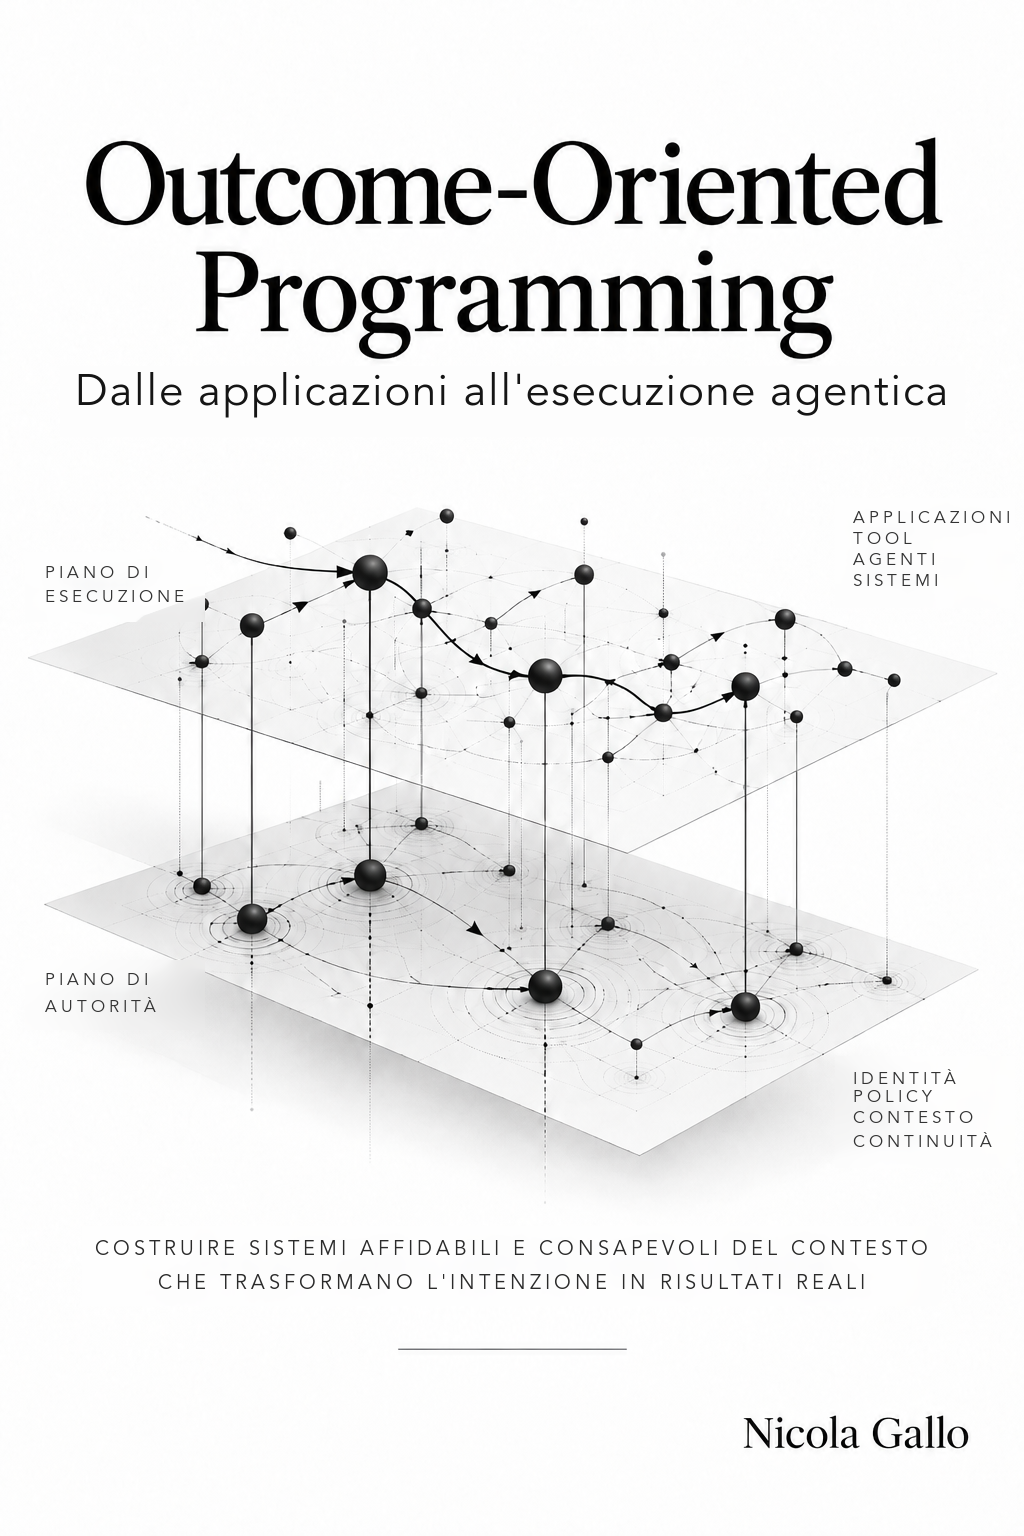
\includegraphics[width=\paperwidth,height=\paperheight]{outcome_oriented_programming_cover.png}
\ifdraftribbon
\begin{tikzpicture}[remember picture, overlay]
  \shade[left color=black!80, right color=black!60] (current page.north west) rectangle ([yshift=-0.6cm]current page.north east);
  \node[anchor=north, text=white, font=\sffamily\footnotesize, inner ysep=4pt]
    at ([xshift=-1.2cm]current page.north) {Lavoro in corso: può contenere errori e sviste e non va considerato una versione definitiva.};
  \shade[top color=red!85!black, bottom color=red!60!black] (current page.north east) -- ([xshift=-2.7cm]current page.north east) -- ([yshift=-2.7cm]current page.north east) -- cycle;
  \node[rotate=-45, text=white, font=\sffamily\bfseries\large, anchor=center]
    at ([xshift=-1.0cm, yshift=-1.0cm]current page.north east) {BOZZA};
\end{tikzpicture}
\fi
\clearpage
\restoregeometry

% ============================================================
% FRONT MATTER
% ============================================================
\frontmatter

% ============================================================
% THESIS STATEMENT - single page
% ============================================================
\thispagestyle{empty}
\vspace*{\fill}
\begin{center}
\begin{minipage}{0.84\linewidth}
\large\itshape\raggedright\setstretch{1.25}
Outcome-Oriented Programming non è la previsione che una particolare architettura prevarrà. È l'ipotesi che, man mano che l'esecuzione diventa più agentica, i sistemi di produzione avranno sempre più bisogno di separare l'interpretazione probabilistica dell'intento dall'esecuzione deterministica, dalla propagazione esplicita dell'autorità, dalla verifica formale e dalla governance.
\end{minipage}
\end{center}
\vspace*{\fill}

\begin{center}
\begin{minipage}{0.84\linewidth}
\hrule\vspace{7pt}
{\small\setstretch{1.02}
\textbf{\sffamily Nota sulla terminologia.} \emph{Outcome-Oriented Programming} si potrebbe rendere in italiano come \emph{programmazione orientata al risultato}: si programma il risultato che deve diventare vero, non la procedura che lo produce. Il nome resta in inglese perché identifica la proposta architetturale descritta in questo libro, non è una descrizione generica. Per la stessa ragione restano in inglese i termini tecnici che in italiano non hanno un equivalente consolidato, come \emph{tool}, \emph{runtime}, \emph{gate}, \emph{lineage}, \emph{prompt} e \emph{governance}, mentre è tradotto tutto ciò che ha una resa naturale: intento, risultato, autorità, contenimento, verifica. Il Glossario in fondo al volume raccoglie entrambi.
\par}
\end{minipage}
\end{center}
\vspace*{0.9in}
\clearpage

% ============================================================
% WHY THIS BOOK EXISTS - concise orientation pages
% ============================================================
\pagestyle{empty}
\vspace*{0.01in}
{\sffamily\bfseries\LARGE Outcome-Oriented Programming\par}
\vspace{0.05in}
{\sffamily\large Dalle applicazioni all'esecuzione agentica\par}
\vspace{0.14in}

{\sffamily\bfseries\Large Perché esiste questo libro\par}
\vspace{0.06in}

{\small\setstretch{0.93}\setlength{\parskip}{0.4pt}
Organizzazioni di ogni dimensione, dalle startup alle grandi imprese, stanno già portando i \textbf{large language model nello sviluppo software e nelle operations}: generano codice, test, documentazione e refactoring; assistono il debugging; alimentano chatbot e automatizzano il supporto. Questo cambia la velocità della produzione del software, ma non ancora la sua struttura di fondo. L'organizzazione continua a costruire l'applicazione in anticipo e a gestirla in esercizio; l'utente, in seguito, la usa, entro il comportamento che è stato definito a monte. Per un'impresa la posta in gioco è più alta: essa gestisce già processi di business, know-how, servizi e controlli, e il valore reale sta nel \textbf{permettere agli agenti AI di agire su quei processi esistenti}.

\textbf{L'esecuzione agentica è il passo successivo.} Invece di chiedere all'AI di aiutare a costruire software per una richiesta futura, l'utente chiede direttamente a un agente un risultato. Nel limite teorico, l'agente interpreta la richiesta, decide che cosa deve accadere, crea o compone la logica di esecuzione mancante, invoca tool e sistemi, si adatta alle evidenze a runtime e restituisce il risultato. L'applicazione pre-costruita smette di essere un oggetto intermedio necessario.

Prima che qualsiasi esecuzione abbia inizio, il prompt deve diventare un \textbf{intento}. Per farsi un'immagine, si immagini di essere appena saliti su un taxi. Si dice dove si vuole andare. L'autista ricava due cose insieme: sul \textbf{lato applicativo}, la destinazione, cioè l'intento e il risultato desiderato; sul \textbf{lato della sicurezza}, che cosa si ha il diritto di chiedergli, cioè il contesto di autorità. Poi l'autista propone un percorso: «allora, di qua, per questa strada?» Quella proposta è il \textbf{piano}. Il nostro «sì» è la sua \textbf{approvazione}. Solo dopo comincia il viaggio.

\begin{center}
\resizebox{0.70\linewidth}{!}{%
\begin{tikzpicture}[
  lbl/.style={font=\sffamily\scriptsize, text=black!60}
]
\node[smallbox, text width=12mm] (prompt) at (0,0) {Prompt};
\node[smallbox, text width=17mm] (interp) at (1.95,0) {Interpretazione\\AI};
\node[smallbox, text width=21mm] (intent) at (4.65,0.8) {Intento +\\risultato desiderato};
\node[authority, text width=21mm] (auth) at (4.65,-0.8) {Contesto di\\autorità $C_0$};
\node[smallbox, text width=21mm] (plan) at (7.4,0) {Piano proposto\\«Allora, di qua?»};
\draw[line width=2.4pt] (9.1,-0.6) -- (9.1,0.6);
\node[lbl, anchor=south] at (9.1,0.65) {approvazione del piano};
\node[lbl, anchor=north] at (9.1,-0.65) {«Sì.»};
\node[lbl, anchor=south] at (4.65,1.3) {lato applicativo};
\node[lbl, anchor=north] at (4.65,-1.3) {lato dell'autorità};
\draw[arrow] (prompt) -- (interp);
\draw[arrow] (interp.east) -- (intent.west);
\draw[arrow] (interp.east) -- (auth.west);
\draw[arrow] (intent.east) -- (plan.west);
\draw[arrow] (auth.east) -- (plan.west);
\draw[arrow] (plan) -- (9.05,0);
\draw[arrow] (9.15,0) -- (10.1,0);
\node[lbl, anchor=west, align=left] at (10.15,0) {la strada\\comincia};
\end{tikzpicture}}
\captionof*{figure}{Dal prompt all'intento e all'autorità: l'interpretazione fissa la destinazione sul lato applicativo e il contesto di autorità sul lato della sicurezza; il piano viene poi proposto («allora, di qua?») e approvato («sì») prima che l'esecuzione abbia inizio.}
\end{center}

Si pensi ora all'esecuzione stessa come a una \textbf{strada}. Intento e autorità sono il punto in cui la strada comincia; il risultato è il punto in cui deve arrivare. Lungo il percorso l'AI compie scelte alle biforcazioni e usa i \textbf{tool deterministici} che si trovano ai bordi della strada. \textbf{La continuità dell'autorità è una dimensione della sicurezza}: viene verificata a ogni passo, e i \textbf{guardrail} mantengono ogni scelta dentro lo spazio ammissibile. Se l'esecuzione ha l'autorità di usare un tool e quel tool non richiede alcuna decisione di policy, la sicurezza è sufficiente e la strada prosegue. \textbf{I gate sono governance}: confini espliciti in cui una policy di controllo richiede una decisione prima che il viaggio possa continuare. Chi sale sul taxi può essere una persona a una scrivania, una persona al telefono, un server o un workload cloud che dialoga da macchina a macchina, un veicolo autonomo, un robot, una macchina in uno stabilimento, un dispositivo domestico: \textbf{ognuno di essi può originare un intento e la sua autorità}, e ognuno di essi può essere il punto in cui la strada arriva. Per questo l'architettura di questo libro non distingue, nel suo nucleo, tra attori software e attori fisici: quella che oggi è un'integrazione tra software e mondo fisico diventa, su questa strada, \textbf{una sola esecuzione che attraversa entrambi}.

\begin{center}
\resizebox{0.62\linewidth}{!}{%
\begin{tikzpicture}[
  thing/.style={draw=black, rounded corners=1pt, align=center, inner sep=2pt, font=\sffamily\scriptsize, minimum height=7mm, text width=12.5mm},
  tool/.style={draw=black, fill=white, rounded corners=1pt, align=center, inner sep=1.5pt, font=\sffamily\tiny, minimum height=4.5mm, text width=11mm},
  lbl/.style={font=\sffamily\scriptsize, text=black!60}
]
% road
\fill[black!6] (1.0,-0.6) rectangle (11.0,0.6);
\draw[line width=1.3pt] (1.0,0.6) -- (11.0,0.6);
\draw[line width=1.3pt] (1.0,-0.6) -- (11.0,-0.6);
\draw[dash pattern=on 3pt off 3pt, black!35] (1.0,0) -- (11.0,0);
\node[lbl, anchor=west] at (1.08,0.42) {trasporto};
% guardrail labels (right end, outside the road)
\node[lbl, anchor=south east, align=right] at (11.0,0.65) {guardrail:\\contenimento applicativo};
\node[lbl, anchor=north east, align=right] at (11.0,-0.65) {guardrail:\\continuità dell'autorità (PIC)};
% intent / outcome
\node[smallbox, text width=13mm] (intent) at (0.0,0) {Intento +\\autorità};
\node[smallbox] (outcome) at (11.95,0) {Risultato};
\draw[arrow] (intent.east) -- (1.0,0);
\draw[arrow] (11.0,0) -- (outcome);
% decision points with forks
\foreach \x in {2.6,6.4,8.7}{
  \node[dot] at (\x,0) {};
  \draw[thinarrow, black!70] (\x,0) -- (\x+0.7,0.3);
  \draw[thinarrow, black!70] (\x,0) -- (\x+0.7,-0.3);
}
\node[lbl, anchor=east] at (2.5,-0.42) {decisione};
% gates
\foreach \x in {4.7,10.3}{
  \draw[line width=2.4pt] (\x,-0.6) -- (\x,0.6);
}
\node[lbl, anchor=west] at (4.8,-0.42) {gate};
\node[lbl, anchor=east] at (10.2,0.42) {gate};
% deterministic tools: small boxes sitting on the road edges
\node[lbl, anchor=south west] at (1.0,1.14) {tool deterministici che l'esecuzione può usare};
\node[tool, anchor=south] at (1.9,0.63) {cerca};
\node[tool, anchor=south] at (3.7,0.63) {scrivi};
\node[tool, anchor=south] at (5.8,0.63) {preventiva};
\node[tool, anchor=south] at (7.6,0.63) {acquista};
\node[tool, anchor=north] at (2.0,-0.63) {leggi};
\node[tool, anchor=north] at (3.8,-0.63) {notifica};
\node[tool, anchor=north] at (5.6,-0.63) {registra};
\node[tool, anchor=north] at (7.3,-0.63) {salva ricevuta};
% actors: who originates intent and authority, and who receives the outcome
\draw[dash pattern=on 2pt off 2pt, black!45] (-0.7,-1.3) -- (12.7,-1.3);
\node[thing] at (1.6,-1.85) {Persona alla\\scrivania};
\node[thing] at (3.07,-1.85) {Persona al\\telefono};
\node[thing] at (4.53,-1.85) {Server /\\workload};
\node[thing] at (6.0,-1.85) {Veicolo\\autonomo};
\node[thing] at (7.47,-1.85) {Robot};
\node[thing] at (8.93,-1.85) {Macchina /\\IoT};
\node[thing] at (10.4,-1.85) {Casa\\intelligente};
\node[lbl, anchor=north] at (6.0,-2.27) {chi sale sul taxi: le origini dell'intento e dell'autorità, software e fisiche allo stesso modo};
\end{tikzpicture}}
\captionof*{figure}{Un'esecuzione come strada: la strada è il trasporto, l'AI sceglie alle biforcazioni e usa i tool ai bordi; l'autorità è verificata a ogni passo entro i guardrail, i gate sono governance e si trovano solo dove una policy richiede una decisione. Sotto la linea, chi può salire sul taxi.}
\end{center}

\begin{notebox}[Il trasporto non è il modello di sicurezza]
La strada in sé è il \textbf{trasporto}: i protocolli, le code e i canali che portano un'esecuzione da un passo al successivo. Un trasporto deve essere sicuro di per sé: confidenzialità, integrità, autenticazione e privacy di ciò che vi transita sono requisiti della strada, e le sue proprietà possono legittimamente essere input della policy di sicurezza. Il requisito posto qui è più ristretto: \textbf{il trasporto da solo non deve essere preso come prova che un effetto richiesto sia autorizzato}. Quando l'autorizzazione viene inferita implicitamente dalla fiducia nel trasporto, come quando un canale fidato viene assunto come prova che un passo è consentito, una parte della motivazione dell'autorizzazione vive fuori dal modello di autorità; ragionamento, composizione e audit diventano più difficili, e in quegli interstizi tendono a comparire incoerenze e vulnerabilità. Il modello di autorità dovrebbe essere in grado di affermare, nei propri termini e con le eventuali proprietà del trasporto esplicitamente ammesse come input, perché una continuazione è autorizzata. \textbf{Il trasporto muove l'esecuzione e la protegge in transito; da solo non decide che cosa l'esecuzione possa causare.}
\end{notebox}

Quel limite non è un'architettura di produzione. Generare tutto a ogni richiesta aggiunge latenza, costi di inferenza e di validazione, e nuova incertezza. Anche correttezza, sicurezza, governance, compliance e accountability si spostano nel percorso di esecuzione. Il problema ingegneristico diventa dove usare intelligenza aperta e dove riusare software deterministico, delimitato e verificabile.

Outcome-Oriented Programming propone quella separazione:

\begin{center}
\sffamily\bfseries\footnotesize
Prompt $\rightarrow$ Intento + Risultato + Autorità $\rightarrow$ Ontologia $\rightarrow$ IER / Piano\\
$\rightarrow$ Approvazione del piano $\rightarrow$ Tool compatibili $\rightarrow$ Esecuzione $\rightarrow$ Evidenze / Risultato
\end{center}

Il cambiamento modifica anche il significato di fidarsi del software. Digest, firme e provenance della supply chain possono sostenere affermazioni sull'identità dell'artefatto, sulla sua integrità, sul firmatario e sul percorso di rilascio, entro un modello di fiducia. \textbf{Da soli, non stabiliscono il comportamento del programma.} I tool hanno quindi bisogno di semantica esplicita leggibile dalle macchine, di effetti, contratti, invarianti e di un livello di assurance più forte dove il rischio lo giustifica.

L'esecuzione viene allora vincolata in due modi indipendenti. Il \textbf{contenimento applicativo} vincola il comportamento software accettato. Il \textbf{contenimento dell'autorità} vincola ciò che questo lineage di esecuzione può causare; PIC (\url{www.pic-protocol.org}) fornisce il modello temporale dell'autorità per quella dimensione. Le evidenze a runtime alimentano i gate di governance, che decidono sul rischio residuo.

\textbf{Il cambio di paradigma va da un'AI che aiuta a scrivere applicazioni a un'AI che programma risultati sopra un substrato di esecuzione vincolato, riusabile e sempre più verificabile.}
}

\vfill
\clearpage
\pagestyle{fancy}

% ============================================================
% ESSENTIAL PUBLICATION / LICENSE NOTICE
% ============================================================
\thispagestyle{empty}
\vspace*{0.02in}
{\sffamily\bfseries\Large Pubblicazione e diritti\par}
\vspace{0.08in}

{\small\setstretch{0.94}\setlength{\parskip}{1.5pt}
\textbf{Outcome-Oriented Programming: dalle applicazioni all'esecuzione agentica}\\
Prima edizione, 6 settembre 2026.\par

\textbf{Autore e creatore originale:} Nicola Gallo\\
\textbf{Editore / emittente, titolare dei diritti patrimoniali d'autore e licenziante:} Nitro Agility S.r.l.\par

Nicola Gallo è l'autore e ha sviluppato concettualmente i contributi originali presentati in quest'opera. Ai fini della presente pubblicazione, egli agisce in qualità di amministratore di Nitro Agility S.r.l., in nome e per conto della società.\par

Copyright \textcopyright\ 2026 Nitro Agility S.r.l.\par

Salvo dove diversamente indicato, il testo originale, i diagrammi originali e lo pseudocodice e i listati illustrativi originali contenuti in questo libro sono concessi in licenza da Nitro Agility S.r.l. secondo i termini della \textbf{Creative Commons Attribution 4.0 International License (CC BY 4.0)} (Attribuzione 4.0 Internazionale). Il testo legale standard della CC BY 4.0 disciplina tale licenza; la presente pubblicazione non lo sostituisce né lo modifica.\par

Licenza canonica: \url{https://creativecommons.org/licenses/by/4.0/}\par

\textbf{Sorgente ed edizioni del libro:} il sorgente LaTeX, gli errata e le edizioni future di questo libro sono mantenuti all'indirizzo \url{https://github.com/nitroagility/books},\\
nella directory \mono{outcome-oriented-programming}.\par

Attribuzione suggerita: \emph{Nicola Gallo (autore e creatore originale), Outcome-Oriented Programming: dalle applicazioni all'esecuzione agentica, \textcopyright\ 2026 Nitro Agility S.r.l., CC BY 4.0.}\par

Le opere di terzi e il materiale concesso in licenza separatamente restano soggetti ai rispettivi diritti e condizioni. Non viene concesso alcun diritto di brevetto o di marchio, salvo dove espressamente indicato.\par

\textbf{Avvertenza tecnica.} Questo libro presenta ricerche, modelli teorici e proposte architetturali; non costituisce una certificazione né una garanzia che una qualsiasi implementazione sia sicura, corretta, conforme, priva di pericoli o adatta a un particolare contesto di deployment. Le affermazioni matematiche e formali si applicano soltanto ai modelli, alle proprietà, alle assunzioni e agli artefatti dichiarati. I contenuti tecnici sono forniti senza garanzia di accuratezza o completezza; le affermazioni formali restano limitate ai modelli, alle assunzioni, alle proprietà e agli artefatti di riferimento dichiarati. Gli implementatori restano responsabili dei propri sistemi, della loro validazione, della conformità e del rispetto dei diritti di terzi.\par

Le note dettagliate su paternità dell'opera, assistenza dell'AI, responsabilità di implementazione, diritti di terzi e attribuzione sono raccolte nell'\textbf{Appendice A}. La metodologia usata per separare teorema, affermazione implementativa, proposta architetturale e problema aperto è raccolta nell'\textbf{Appendice B}. Una breve corrispondenza, non normativa, con alcuni framework di rischio aziendale è raccolta nell'\textbf{Appendice C}.\par

\textbf{Contatti.} Per contattare l'autore o l'editore:\\
\href{mailto:nicola.gallo@nitroagility.com}{\nolinkurl{nicola.gallo@nitroagility.com}}\\
\href{mailto:info@nitroagility.com}{\nolinkurl{info@nitroagility.com}}\\
\url{https://nitroagility.com/}\par

\textbf{Implementazione.} Il modo di pensare descritto in questo libro viene messo in pratica in Permguard, un progetto open source di autorizzazione di Nitro Agility: \url{https://permguard.com/}.\par
}

\vfill
{\footnotesize Composto in LaTeX. I diagrammi interni sono monocromatici e vettoriali.}
\clearpage

\chapter*{Prefazione}
\addcontentsline{toc}{chapter}{Prefazione}
La transizione visibile all'AI comincia con l'ingresso dei large language model nello sviluppo software e nelle operations. Vale per le startup come per le grandi imprese: i modelli aiutano i programmatori a generare codice, test, documentazione, refactoring e ipotesi di debugging; alimentano chatbot e ottimizzano il supporto; e cambiano in modo sostanziale la velocità e l'economia della produzione del software. Ma è ancora un'evoluzione dentro il familiare modello centrato sull'applicazione: i requisiti vengono trasformati in un'applicazione, l'organizzazione la distribuisce e la gestisce in esercizio, e gli utenti poi la usano entro il comportamento che essa già codifica.

Per un'organizzazione consolidata la questione è più ampia. Un'impresa non parte da una pagina bianca: gestisce già processi di business, know-how accumulato, servizi, controlli e obblighi che precedono qualsiasi nuovo software. Il cambiamento rilevante non riguarda quindi soltanto la velocità con cui il software può essere scritto, ma \textbf{il modo in cui gli agenti AI possono agire direttamente su quei processi esistenti}.

Questo libro si chiede che cosa viene dopo. Il passo più radicale non è un'AI che scrive l'applicazione più in fretta, ma \textbf{un agente AI che riceve direttamente il risultato desiderato e costruisce l'esecuzione necessaria per raggiungerlo}. Nel limite teorico, l'agente può comprendere la richiesta, determinare che cosa deve accadere, generare o comporre la logica di esecuzione mancante, invocare i sistemi necessari, adattarsi ai risultati intermedi e restituire il risultato. Un'applicazione specifica per il compito non dovrebbe più esistere prima della richiesta.

È un'affermazione molto più ampia di «l'AI scrive codice», e richiede una precisazione altrettanto importante. Il substrato computazionale non scompare. Modelli, runtime, sistemi operativi, database, protocolli, servizi, tool, reti e macchine fisiche restano. \textbf{Ciò che diventa opzionale, nel limite teorico, è l'applicazione pre-costruita come oggetto obbligatorio tra un risultato umano e la sua esecuzione.}

La realtà della produzione oppone subito resistenza. La generazione illimitata a runtime sposta lavoro di natura progettuale nel percorso critico dell'esecuzione (hot path): ragionamento, sintesi, validazione, compilazione e verifica consumano tempo e calcolo prima che cominci il lavoro deterministico utile. Sposta inoltre a runtime decisioni che l'ingegneria del software prendeva tradizionalmente prima del deployment. Correttezza, sicurezza, autorità, governance, compliance, evidenze e accountability devono quindi diventare parte dell'esecuzione stessa.

La conseguenza economica è altrettanto importante. Quando esiste già un'operazione stabile, rigenerarla ripetutamente getta via il vantaggio che il software ha sempre tratto dal riuso. L'architettura di produzione dovrebbe quindi spendere intelligenza aperta dove interpretazione e pianificazione sono davvero necessarie, per poi abbassare il risultato in un'esecuzione deterministica o delimitata riusabile ovunque sia possibile.

È questa la tensione da cui prende le mosse Outcome-Oriented Programming. Il limite teorico dice che l'applicazione può scomparire come composizione preliminare obbligatoria. La risposta ingegneristica è selettiva: \textbf{l'intelligenza interpreta e propone; il software riusabile esegue; verificatori e confini di governance decidono quali proposte possono diventare effetti.}

Questo cambiamento espone un divario di fiducia che i normali controlli sugli artefatti non colmano. Le moderne supply chain del software possono usare digest, firme, identità del publisher, provenance e metadati di rilascio per sostenere affermazioni su quale artefatto sia stato ricevuto e se i byte attesi o i percorsi di rilascio siano stati preservati, entro un modello di fiducia. Quei meccanismi sono importanti, ma non sono prove semantiche di ciò che il programma farà. L'esecuzione agentica ha quindi bisogno anche di un livello comportamentale esplicito: semantica leggibile dalle macchine, effetti, precondizioni, postcondizioni, invarianti ed evidenze di assurance legate ai tool che l'esecuzione può comporre.

Un ulteriore cambiamento è temporale. Il software distribuito ha sempre eseguito attraverso il tempo: un produttore agisce ora, un messaggio attende, e un futuro consumatore può non esistere ancora. I sistemi agentici generalizzano quella condizione. Non solo il prossimo esecutore, ma anche la prossima opzione concreta, la prossima evidenza o il prossimo risultato possono essere sconosciuti nel momento in cui l'intento viene espresso. Outcome-Oriented Programming ha quindi bisogno di un modello di esecuzione che resti significativo attraverso confini asincroni e fatti futuri ignoti.

La strada delle pagine di apertura dissolve anche un confine che l'architettura del software ha trattato come fisso. Un'esecuzione può essere originata da, e può arrivare a, una persona che agisce tramite un computer o un dispositivo mobile, un server o un workload cloud che agisce da macchina a macchina, un veicolo autonomo, un robot, una macchina industriale o un oggetto connesso in una casa. Se il significato dell'esecuzione, la sua autorità e la sua governance sono legati al lineage anziché all'applicazione che ospita un passo, allora \textbf{esecutori software ed esecutori fisici non sono due mondi uniti da un'integrazione. Sono posizioni sulla stessa strada.} Questo libro non prevede quanto rapidamente avverrà quella convergenza; sostiene che un'architettura per l'esecuzione agentica non dovrebbe presupporre la distinzione.

Un ulteriore cambiamento riguarda l'autorità. Se un'esecuzione può attraversare applicazioni, servizi, tool, code, agenti e organizzazioni, l'applicazione non è più un confine di sicurezza sufficiente. Non lo è nemmeno il trasporto. Canali, code e protocolli devono essere sicuri di per sé, ma l'autorità di un passo non può essere inferita dal canale su cui è arrivato; \textbf{un modello di sicurezza deve essere in grado di affermare, nei propri termini, perché un passo è autorizzato}. Una singola esecuzione può attraversare molti stack software, mentre un singolo servizio può elaborare contemporaneamente molte esecuzioni non correlate. L'unità significativa diventa il \term{lineage di esecuzione}: la catena causale che comincia con un intento e continua attraverso ogni azione che l'intento causa.

È qui che Provenance Identity Continuity (PIC) diventa centrale. Le risorse pubbliche di PIC sono mantenute all'indirizzo \url{https://www.pic-protocol.org}; l'organizzazione dei sorgenti è \url{https://github.com/pic-protocol}; il portale del modello formale è \url{https://www.pic-protocol.org/formal-model}; e l'articolo teorico è disponibile all'indirizzo \url{https://arxiv.org/abs/2607.08906}. PIC modella l'autorità come qualcosa che deve restare causalmente connesso all'esecuzione che l'ha originata. La stessa esecuzione può essere osservata attraverso due piani paralleli. Il \term{piano applicativo} chiede \emph{che cosa sta facendo il sistema}. Il \term{piano dell'autorità} chiede \emph{che cosa questo specifico lineage è autorizzato a causare}. Descrivono gli stessi eventi da prospettive diverse.


Quella coordinata temporale cambia anche il significato della composizione. Due esecuzioni possono esporre la stessa autorità apparente e rappresentare comunque autorizzazioni diverse, perché la loro autorità discende da cause diverse. Un esecutore che si trova a possedere due autorità indipendentemente valide non è per ciò stesso autorizzato a fonderle dentro un compito arbitrario. Se due lineage vengono combinati intenzionalmente, la combinazione è essa stessa una decisione di sicurezza: la policy deve autorizzare l'incontro, e i lineage che vi contribuiscono devono restare distinguibili. In forma compatta: \textbf{il possesso non autorizza la composizione}.

Questi cambiamenti rendono l'architettura orientata al verificatore. La pianificazione AI resta probabilistica, ma l'accettazione delle transizioni di stato critiche dovrebbe essere tanto deterministica e controllabile quanto la proprietà lo consente. I tool hanno sempre più bisogno di Semantic Manifest e contratti leggibili dalle macchine che descrivano operazioni a livello di ontologia, precondizioni, effetti, postcondizioni, invarianti e le evidenze a sostegno di tali affermazioni. Intento e risultati desiderati possono allora essere abbassati nello stesso sistema di coordinate semantiche prima che avvenga il binding dei tool. Il risultato di quell'abbassamento è un piano compatto, orientato alla macchina, la Intent Execution Representation (IER), la rappresentazione di esecuzione dell'intento, che il runtime valida al posto del linguaggio naturale. I modelli possono proporre interpretazioni semantiche, piani, tool, parametri e continuazioni. Componenti deterministici e, dove praticabile, formalmente verificati decidono se i contratti semantici selezionati, gli invarianti applicativi, le condizioni di autorità e i predicati sulle evidenze valgono prima che quelle proposte diventino esecuzione. Visto dal lato del tool e dal lato dell'origine, quel controllo si presenta così.

\begin{center}
\resizebox{0.96\linewidth}{!}{%
\begin{tikzpicture}[
  layer/.style={draw=black, fill=white, rounded corners=1pt, align=center, inner sep=3pt, font=\sffamily\scriptsize, text width=36mm, minimum height=7mm},
  lbl/.style={font=\sffamily\scriptsize, text=black!60, align=center}
]
% origin (left)
\node[smallbox, text width=26mm] (intent) at (0,1.0) {Intento +\\predicato di risultato};
\node[authority, text width=26mm] (auth) at (0,-0.45) {Contesto di\\autorità $C_0$};
\node[lbl, anchor=north] at (0,-1.1) {origine: che cosa l'esecuzione\\può significare e può causare};
% tool (right)
\node[layer] (id) at (9.0,1.35) {Identità dell'artefatto\\digest, firma, provenance della supply chain};
\node[layer] (man) at (9.0,0.25) {Semantic Manifest\\operazione, effetti, contratti, invarianti};
\node[layer] (asr) at (9.0,-0.85) {Evidenze di assurance\\verifica formale, raffinamento, test};
\node[draw=black!50, fill=black!3, rounded corners=2pt, fit=(id)(man)(asr), inner sep=4pt] (tool) {};
\node[layer] at (9.0,1.35) {Identità dell'artefatto\\digest, firma, provenance della supply chain};
\node[layer] at (9.0,0.25) {Semantic Manifest\\operazione, effetti, contratti, invarianti};
\node[layer] at (9.0,-0.85) {Evidenze di assurance\\verifica formale, raffinamento, test};
\node[lbl, anchor=south] at (tool.north) {Tool $T$: affermazioni legate a un'origine verificata};
% agent + verifier (center)
\node[box, text width=33mm] (agent) at (4.5,1.35) {L'agente AI propone\\il passo successivo: usare $T$};
\node[box, text width=33mm] (ver) at (4.5,-0.45) {Verificatore deterministico\\dentro l'intento?\\dentro l'autorità?\\dentro il contratto di $T$?};
\node[smallbox, text width=24mm] (exec) at (4.5,-2.15) {passo accettato\\$\rightarrow$ esecuzione};
\node[smallbox, text width=14mm] (rej) at (1.3,-2.15) {rifiutato};
\draw[arrow] (agent) -- (ver);
\draw[arrow] (ver) -- node[right, font=\sffamily\scriptsize, text=black!60] {accetta} (exec);
\draw[dashedarrow] (ver.south west) -- (rej.north east);
\draw[arrow] (intent.east) to[out=0,in=180] (ver.west |- intent.east);
\draw[arrow] (auth.east) -- (ver.west |- auth.east);
\draw[arrow] (tool.west |- ver.east) -- (ver.east);
\node[lbl, anchor=north] at (9.0,-1.6) {il controllo è un'accettazione a livello di protocollo,\\non un giudizio lasciato al modello};
\end{tikzpicture}}
\captionof*{figure}{Esecuzione orientata al verificatore. Un tool porta con sé la propria identità di artefatto, il proprio Semantic Manifest e le proprie evidenze di assurance, tutti legati a un'origine verificata. Prima che un passo proposto diventi esecuzione, un verificatore deterministico controlla che esso sia semanticamente dentro l'intento, dentro il contesto di autorità e dentro il contratto del tool. Quell'accettazione vive a livello di protocollo, non nella confidenza del modello.}
\end{center}

In forma compatta, il percorso di esecuzione proposto è:

\begin{center}
\sffamily\bfseries\footnotesize
Prompt $\rightarrow$ Intento + Risultato desiderato + Autorità $\rightarrow$ Ontologia $\rightarrow$ IER / Piano\\
$\rightarrow$ Approvazione del piano $\rightarrow$ Tool semanticamente compatibili\\
$\rightarrow$ Esecuzione $\rightarrow$ Evidenze $\rightarrow$ Risultato
\end{center}

La mappatura semantica non è una semplice comodità di ricerca. È il ponte tra ciò che l'utente intende e ciò che i componenti eseguibili dichiarano di fare. Un tool non viene selezionato soltanto perché un agente prevede che sia utile. Il suo Semantic Manifest dovrebbe dichiarare l'operazione a livello di ontologia che implementa, le sue precondizioni, gli effetti, le postcondizioni, gli invarianti e le evidenze di assurance a sostegno di tali affermazioni. Verifica formale, verifica a runtime, test, attestazione o altri meccanismi di assurance possono allora essere agganciati ad affermazioni specifiche anziché a una vaga etichetta di «software fidato».

Questo crea due problemi di contenimento indipendenti che si incontrano nello stesso evento di esecuzione. Il \term{contenimento applicativo} chiede se il tool e la transizione selezionati restino dentro il contratto semantico e comportamentale accettato. Il \term{contenimento dell'autorità} chiede se questo specifico lineage di esecuzione sia autorizzato a causare la transizione; PIC affronta la seconda domanda attraverso la continuità causale e l'autorità non espansiva. Nessuna delle due proprietà sostituisce l'altra.

Come predicato architetturale di accettazione, un passo critico può quindi essere scritto schematicamente come segue.
\begin{formulabox}[Predicato di accettazione per un passo critico]
\[
\begin{aligned}
\operatorname{Accept}_i ={}&
\operatorname{SemanticCorrect}_i \land
\operatorname{OutcomeCompatible}_i\\
&{}\land \operatorname{AuthorityValid}_i \land
\operatorname{PolicyAcceptable}_i.
\end{aligned}
\]
\end{formulabox}
Questa espressione è una decomposizione progettuale, non l'affermazione che tutti e quattro i predicati siano automaticamente decidibili o formalmente provati in ogni deployment. Il punto è rendere espliciti gli obblighi di prova e l'incertezza residua.

L'esecuzione produce allora evidenze, e non soltanto effetti collaterali: costo, latenza, effetti osservati, stato della policy, stato di compliance, stato di assurance, indicatori di rischio e avanzamento verso il risultato desiderato. Quelle osservazioni possono alimentare KPI/KRI di governance ed Execution Gate. Dove il rischio residuo è accettabile, l'esecuzione può continuare; dove è condizionatamente accettabile, il runtime può vincolare, validare o fare escalation; dove è inaccettabile, la transizione può essere negata o reindirizzata verso un percorso autorizzato separatamente. \emph{L'architettura non promette quindi un rischio residuo nullo.} Cerca di convertire una parte maggiore di quel rischio da speranza implicita sul comportamento del modello in qualcosa che possa essere \textbf{delimitato, verificato, osservato e governato}.

Anche lo human-in-the-loop cambia significato nella stessa architettura. Un essere umano non ha bisogno di rivedere ogni riga generata da un'AI. L'esecuzione può fermarsi a un gate quando raggiunge un confine di autorità, di rischio, di compliance o di policy. Quel gate può essere valutato da una policy deterministica, da agenti di governance specializzati, da un essere umano o da una combinazione di questi. Gli esseri umani restano dove un'organizzazione richiede deliberatamente autorità, giudizio o accountability umani.

\noindent\begin{minipage}{\linewidth}
La tesi del libro può essere enunciata in otto punti:

{\sffamily\small
\begin{itemize}\setlength{\itemsep}{1pt}\setlength{\parskip}{0pt}
\item I risultati sostituiscono i workflow pre-costruiti come punto di partenza.
\item L'intento viene abbassato in una semantica esplicita.
\item Gli agenti propongono la composizione.
\item I tool verificati svolgono il lavoro stabile.
\item Comportamento applicativo e autorità sono vincolati separatamente.
\item I lineage preservano la causalità attraverso il tempo.
\item Autorità indipendenti si incontrano solo attraverso una composizione esplicita.
\item La governance controlla il rischio residuo e la continuazione.
\end{itemize}}
\end{minipage}
\vspace{2pt}


Il risultato non è semplicemente «un'AI che scrive software». È un passaggio dal software centrato sull'applicazione a un'esecuzione centrata sul risultato, consapevole del lineage e orientata al verificatore.

\tableofcontents
\clearpage

\chapter*{Come leggere questo libro}
\addcontentsline{toc}{chapter}{Come leggere questo libro}
Il libro è organizzato come una progressione architetturale, non come il manuale di un prodotto.

La \textbf{Parte I} parte dal limite agentico teorico: un risultato può essere richiesto prima che esista un'applicazione specifica per il compito, e il software può essere sintetizzato come parte dell'esecuzione. Spiega poi perché quel limite non è un'architettura di produzione -- governance, sicurezza, compliance, correttezza, latenza ed economia impongono una nuova separazione tra proposta probabilistica ed esecuzione deterministica e verificabile -- prima di definire Outcome-Oriented Programming. Legge inoltre la transizione in chiave economica: le finestre di arbitraggio, la ristrutturazione del mercato e delle competenze, e la sovranità digitale come opportunità parallela. Quei passaggi sono la lettura economica dell'autore, non affermazioni architetturali.

La \textbf{Parte II} introduce l'esecuzione attraverso il tempo: i tool, i Semantic Manifest, il binding semantico basato su ontologia, la Intent Execution Representation, i tre problemi N+1, i lineage di esecuzione e l'architettura a due piani.

La \textbf{Parte III} introduce il modello di autorità: PIC, provenance contro continuità, la distinzione tra possesso e composizione, la lettura temporale del confused deputy, il ponte di exchange PIC-X ad alto livello, i confini riceventi, i Composition Gate espliciti, le decisioni differite e la Governance Intelligence.

La \textbf{Parte IV} assembla questi concetti in un Intent Runtime verificabile. Separa interpretazione e pianificazione probabilistiche da binding semantico e accettazione deterministica, introduce una scala di assurance che va dall'integrità dell'artefatto al raffinamento formale, e spiega i ruoli complementari di Lean, Tamarin e ProVerif prima di tornare all'economia dell'esecuzione, alla revisione semantica e al ruolo mutevole del programmatore.

La \textbf{Parte V} guarda oltre l'attuale confine dell'applicazione ed enuncia in forma compatta i principi di progettazione dell'architettura.

Due immagini delle pagine di apertura ricorrono in tutto il libro. Il \emph{taxi} rappresenta la trasformazione di un prompt in un intento, un contesto di autorità e un piano approvato. La \emph{strada} rappresenta l'esecuzione stessa: il trasporto che la porta, i guardrail e i gate che la delimitano, e gli esecutori software e fisici che incontra lungo il cammino.

I diagrammi usano deliberatamente soltanto riquadri, linee, frecce e scala di grigi. L'architettura dovrebbe essere comprensibile senza dipendere da un fornitore, un linguaggio di programmazione, un cloud, un framework per agenti o una particolare tecnologia di implementazione.

Le note dettagliate su aspetti legali, diritti e assistenza dell'AI sono raccolte nell'Appendice A. La disciplina delle fonti e delle affermazioni, inclusi i riferimenti pubblici di PIC e le impronte (fingerprint) degli artefatti formali, è raccolta nell'Appendice B. L'Appendice C fornisce una breve corrispondenza, non normativa, con alcuni framework di rischio aziendale, così che l'argomentazione principale resti architetturale anziché orientata alla compliance.

% ============================================================
% PART I
% ============================================================
\mainmatter
\part{Quando l'applicazione smette di essere l'unità}

\chapter{Al limite, l'applicazione scompare}

La transizione visibile dell'AI inizia con l'ingegneria del software assistita da LLM. Un modello aiuta uno sviluppatore a generare codice, test, documentazione, refactoring o ipotesi di debugging, e risponde agli utenti attraverso chatbot e assistenza automatizzata. Lo sviluppo diventa più rapido e il supporto più efficiente per l'utente, ma l'architettura è ancora quella familiare:

\begin{center}
\sffamily\bfseries
Requisito $\rightarrow$ Sviluppatore + LLM $\rightarrow$ Codice $\rightarrow$ Applicazione $\rightarrow$ Utente
\end{center}

Si tratta di un cambiamento importante nella produttività e nei risparmi economici, ma non ancora di un cambiamento ontologico. L'organizzazione continua a costruire e a distribuire un'applicazione prima che l'utente possa ottenere, attraverso di essa, il risultato di business.

Disegnato su un asse temporale, il guadagno è un insieme di segmenti più corti: dal requisito al codice, e il supporto che segue l'utente.

\begin{figure}[H]
\centering
\resizebox{0.92\linewidth}{!}{%
\begin{tikzpicture}[
  seg/.style={draw=black, anchor=west, minimum height=5.5mm, inner sep=0pt, font=\sffamily\scriptsize, align=center},
  rl/.style={font=\sffamily\footnotesize, anchor=east},
  lbl/.style={font=\sffamily\scriptsize, text=black!60}
]
% row 1
\node[rl] at (-0.25,0) {Sviluppatore};
\node[seg, fill=black!22, minimum width=6.0cm] at (0,0) {Codice};
\node[seg, fill=black!8, minimum width=2.6cm] at (6.0,0) {Applicazione};
\node[seg, fill=white, minimum width=1.6cm] at (8.6,0) {Utente};
\node[seg, fill=black!14, minimum width=2.2cm] at (10.2,0) {Supporto};
% row 2
\node[rl] at (-0.25,-1.0) {Sviluppatore + LLM};
\node[seg, fill=black!22, minimum width=3.0cm] at (0,-1.0) {Codice};
\node[seg, fill=black!8, minimum width=2.6cm] at (3.0,-1.0) {Applicazione};
\node[seg, fill=white, minimum width=1.6cm] at (5.6,-1.0) {Utente};
\node[seg, fill=black!14, minimum width=1.2cm] at (7.2,-1.0) {Supporto};
% saved span
\draw[dashed, black!50] (12.4,0.3) -- (12.4,-1.6);
\draw[dashed, black!50] (8.4,-0.7) -- (8.4,-1.6);
\draw[{Latex[length=1.6mm]}-{Latex[length=1.6mm]}, black!70] (8.45,-1.45) -- (12.35,-1.45);
\node[lbl, anchor=south] at (10.4,-1.4) {tempo e costo risparmiati};
% axis
\draw[arrow] (0,-2.0) -- (13.4,-2.0);
\node[lbl, anchor=north] at (0,-2.05) {requisito};
\node[lbl, anchor=north east] at (13.4,-2.05) {time to market, costo};
\end{tikzpicture}}
\caption{Stessa architettura, segmenti più corti: l'LLM riduce la distanza dal requisito al codice, e il supporto che segue l'utente. Non usarlo non è una scelta neutra: è una perdita di tempo e di costo rispetto a chi lo usa.}
\end{figure}

C'è anche una lettura economica di questo primo passo. Quanto segue nei passaggi economici di questo capitolo è la lettura, da parte dell'autore, di pattern di mercato che l'industria ha già vissuto; non è un'affermazione architetturale, e l'Appendice~\ref{app:claims} la classifica separatamente. Man mano che Sviluppatore + LLM diventa ampiamente disponibile, una capacità che tutti possiedono può cessare di essere un fattore di differenziazione durevole: \textbf{il valore tende a spostarsi altrove}. Dove si sposti non è ancora stabilito. Una produzione più economica può semplicemente significare più software in totale, così che i programmatori restino necessari come prima. Oppure la frontiera può spostarsi verso un tipo diverso di software, e in quel caso la corsa è a creare quel nuovo tipo anziché a ottimizzare la produzione del vecchio; e se è così, la prima domanda è chi sia in grado di scriverlo. Le persone con le competenze per farlo potrebbero essere poche; oppure potrebbero essere proprio quelle lasciate a casa nella fase di taglio dei costi, che altri raccoglieranno presto e a prezzo di saldo. La competizione per i talenti di ricerca scarsi attorno ai modelli stessi illustra come una capacità complementare possa diventare strategicamente preziosa. Altri esiti sono possibili e non ancora visibili. L'argomento strategico avanzato qui è che trattare la commodity stessa come il vantaggio, come se una generazione più rapida delle stesse applicazioni avesse chiuso la questione, significa fraintendere la transizione.

Questi passaggi sono analisi di scenario, non affermazioni che gli esiti descritti in termini di mercato, occupazione, organizzazione o tecnologia si verificheranno con certezza. Esiti alternativi sono possibili, e i tempi, l'entità e la direzione di questi effetti possono differire tra settori, giurisdizioni, organizzazioni e condizioni tecnologiche.

Il risparmio può essere temporaneo come fonte di margine differenziale, ed è questo il punto attorno a cui ruota il resto del capitolo. Finché pochi hanno la capacità, il minor costo di sviluppo resta a chi la possiede, come margine. Man mano che la capacità si diffonde, la pressione competitiva tende a trasferire parte di quella riduzione di costo ai clienti, attraverso prezzi più bassi, consegne più rapide, qualità più alta o maggiore output: qualcuno abbassa i prezzi per conquistare clienti, e gli altri devono rispondere. È ciò che la concorrenza ha di solito fatto delle riduzioni di costo che tutti possono ottenere. Quanta parte del guadagno resti come margine dipende dalla struttura del mercato, dalla domanda, dalla differenziazione, dai contratti e dalle scelte organizzative; ma dove la concorrenza funziona, il risparmio smette di essere margine e diventa \textbf{il nuovo prezzo del software}. Visto dal lato del cliente, lo stesso fatto si legge come la fine di un premio. I prezzi di un settore tendono ad assestarsi sul suo processo produttivo: il cliente paga per i passi che il processo contiene. Il prezzo del software come codice scritto incorporava un premio per uno di quei passi, il lavoro scarso di chi scrive codice a mano. Quando un passo scompare dal processo, il prezzo di quel passo tende a scomparire con esso, e pochi pagheranno in seguito per un pezzo di lavoro che non esiste più, a meno che il prodotto stesso non sia cambiato. Quel premio era a sua volta un arbitraggio, nel senso lato usato qui, tra quanto costava produrre il codice e quanto i clienti erano abituati a pagarlo, e si restringe man mano che la differenza diventa visibile e sfruttabile. Un'organizzazione che aspetti quel momento per finanziare il proprio passo successivo può scoprire che il denaro su cui contava è già andato in prezzo, e può trovarsi ad affrontare la vera innovazione, quella descritta nella prossima sezione, con gli stessi vincoli di budget di prima e un mercato che si è già mosso. La finestra in cui il risparmio può essere speso è la finestra in cui non tutti lo hanno ancora. Le organizzazioni possono consumare, distribuire, trattenere o reinvestire quel guadagno. \textbf{L'ipotesi avanzata qui è che reinvestirne una parte finché esiste migliori la preparazione all'esecuzione agentica}; un'organizzazione che si limiti a trasferirlo al prezzo rinuncia al denaro e, se la transizione si concretizza, resta anche indietro rispetto a chi lo ha usato per costruire ciò che viene dopo.

\keyidea{In termini semplici: se lo sviluppo assistito da LLM riduce il costo di consegna di parte del software, un'organizzazione può temporaneamente catturare parte di quel guadagno come margine. Il guadagno può essere trasferito ai clienti, trattenuto, allocato altrove o reinvestito. Questo libro sostiene che almeno una parte vada trattata come l'opportunità di costruire le capacità che un modello di esecuzione più agentico potrebbe richiedere; chi lo tiene solo come margine può vederselo eroso dalla concorrenza, senza aver costruito nulla in cambio.}

Un board può ragionevolmente leggere questa fase, dal proprio punto di osservazione, principalmente come una voce di risparmio: lo stesso output con meno persone, o con persone meno costose. Quella lettura non è un errore del board. L'informazione di cui ha bisogno è tecnica, e può venire soltanto dalla leadership tecnica, che può aggiungere una seconda prospettiva: che parte del risparmio può essere temporanea, che un ulteriore cambiamento nel modello di esecuzione potrebbe richiedere investimenti prima che il suo valore economico sia visibile, e che il margine di questa fase può essere il finanziamento della prossima. \textbf{Dove quella seconda prospettiva non viene comunicata, la responsabilità è della leadership tecnica}, e l'organizzazione può sottoinvestire in capacità che in seguito si rivelano importanti; un board a cui è stato detto solo del risparmio chiederà, con ragione, perché le persone il cui compito era vedere arrivare il cambiamento non lo abbiano detto. Si tratta di un rischio strategico qui identificato, non di una previsione su ogni board o su ogni responsabile tecnico.

\begin{notebox}[La finestra di arbitraggio]
Una commodity non è un vantaggio durevole, ma non tutti la possiedono ancora. Finché l'adozione è disomogenea, chi usa lo sviluppo assistito da LLM e chi non lo usa corrono a \textbf{due velocità diverse e con due basi di costo diverse} (Figura~\ref{fig:arbitrage}). Questo sembra concorrenza, ma si comporta come arbitraggio, e il termine è usato per analogia e non nel senso finanziario stretto: il guadagno deriva da una differenza di prezzo sulla stessa capacità, e dura solo quanto dura la differenza. Un vantaggio di adozione tende a restringersi man mano che la capacità si diffonde, anche se differenze successive di costo, qualità, regolamentazione, accesso o asset complementari possono creare nuovi differenziali. Le grandi organizzazioni, rallentate da regolamentazione, compliance e procedure, possono entrare tardi e perdere terreno rispetto a player più piccoli, per i quali la finestra è anche un'occasione per recuperare su concorrenti con più risorse. Ogni finestra tende a restringersi una volta sola, su una capacità; quando tutti hanno quella capacità, è una commodity nel senso pieno. La finestra successiva, se arriva, si apre su una capacità diversa, come sostiene la prossima sezione. Il punto strategico utile è che un'adozione disomogenea può creare un vantaggio temporaneo; la sua durata e la sua entità sono empiriche, non predeterminate. Sembra che ci troviamo ora in quella fase: l'adozione è ancora disomogenea e il mercato si sta segmentando.
\end{notebox}

\begin{figure}[H]
\centering
\resizebox{0.9\linewidth}{!}{%
\begin{tikzpicture}[lbl/.style={font=\sffamily\scriptsize, text=black!60}]
% shaded window
\begin{scope}[on background layer]
\fill[black!9] (0,0.8) .. controls (1.5,0.8) and (2.2,2.8) .. (4,2.8) -- (8,2.8) .. controls (6.0,2.8) and (5.0,0.8) .. (3.5,0.8) -- cycle;
\end{scope}
% axes
\draw[arrow] (0,0) -- (9.8,0);
\node[lbl, anchor=north east] at (9.8,-0.08) {tempo};
\draw[arrow] (0,0) -- (0,3.7);
\node[lbl, anchor=south, rotate=90] at (-0.3,1.85) {valore per l'utente per unità di tempo e costo};
% curves
\draw[line width=0.9pt] (0,0.8) .. controls (1.5,0.8) and (2.2,2.8) .. (4,2.8) -- (9.5,2.8);
\draw[line width=0.9pt, dashed] (0,0.8) -- (3.5,0.8) .. controls (5.0,0.8) and (6.0,2.8) .. (8,2.8) -- (9.5,2.8);
\node[font=\sffamily\scriptsize, anchor=south east] at (3.9,2.85) {chi adotta};
\node[font=\sffamily\scriptsize, anchor=north west] at (4.4,0.75) {chi non adotta, più tardi};
% gap
\draw[{Latex[length=1.6mm]}-{Latex[length=1.6mm]}, black!70] (5.0,0.95) -- (5.0,2.65);
\node[lbl, anchor=east, align=right] at (4.85,1.8) {due velocità,\\due basi di costo};
% now
\draw[dashed, black!50] (2.4,0) -- (2.4,3.1);
\node[lbl, anchor=south] at (2.4,3.12) {oggi};
% window bracket
\draw[black!60] (1.0,3.45) -- (8.0,3.45);
\draw[black!60] (1.0,3.35) -- (1.0,3.55);
\draw[black!60] (8.0,3.35) -- (8.0,3.55);
\node[lbl, anchor=south] at (4.5,3.5) {finestra di arbitraggio: si restringe al diffondersi dell'adozione};
% commodity
\node[lbl, anchor=north, align=center] at (8.9,2.7) {commodity:\\uguale per tutti};
\end{tikzpicture}}
\caption{La finestra di arbitraggio: finché l'adozione è disomogenea, chi adotta consegna all'utente più valore per unità di tempo e costo di chi non adotta. Il divario è una competizione temporale ed economica; tende a restringersi man mano che l'adozione si generalizza e la capacità diventa una commodity.}
\label{fig:arbitrage}
\end{figure}

Il mercato resta instabile, e questo libro legge la confusione come un sintomo della stessa fase: l'attenzione va all'effetto piccolo, il codice più economico, più che a quello grande, il cambiamento di unità che il resto di questo capitolo descrive. Lo sviluppo di modelli di frontiera può restare concentrato tra relativamente pochi attori a causa dei suoi requisiti insolitamente esigenti. Attorno a essi, le strategie attuali vanno dall'ottimizzare modelli che non si sono costruiti, a prodotti basati su API presentati come una strategia AI, al tooling del momento. Molte di queste sono posizioni della fase più che del mercato che la segue: esistono perché lo strato non è ancora una commodity, e potrebbero assottigliarsi quando lo sarà, come si assottigliarono le attività costruite sulla rivendita di banda o sull'hosting di un singolo server quando connettività e hosting divennero commodity. Questo libro si concentra su una diversa possibile fonte di valore durevole: il substrato su cui l'esecuzione agentica può girare, e le persone in grado di costruirlo.

\begin{notebox}[L'arbitraggio dell'accesso]
Un secondo arbitraggio potrebbe correre tra chi ha accesso a un modello sufficientemente capace e chi no. Se l'accesso è scarso o prezzato in modo asimmetrico, le organizzazioni con costi di accesso materialmente inferiori possono ottenere un vantaggio temporaneo; la sua durata dipende da offerta, concorrenza, alternative, investimenti in infrastruttura, modelli open, regolamentazione e cambiamento tecnologico. È anche l'arbitraggio più ampiamente compreso, ed è per questo che difficilmente verrà lasciato aperto: gran parte dell'industria compete per gli stessi input, le GPU, le materie prime e l'energia che stanno dietro di esse, i data center che le ospitano e i modelli che servono. La corsa esiste proprio perché l'accesso è un vantaggio che pochi si aspettano di mantenere incontestato. Se chi detiene quell'accesso scegliesse di non concederlo, di non venderlo a chi ne è privo, o di venderlo a un prezzo che gli altri non possono sostenere, il vantaggio sarebbe suo per tutto il tempo necessario agli altri per costruirsi il proprio, ed è una delle ragioni per cui gli altri stanno costruendo. Vale la pena enunciare il meccanismo: chi costruisce servizi sopra un modello paga per la capacità sottostante, e se quel costo differisce abbastanza tra concorrenti, la sola differenza può espellere dal mercato quello svantaggiato, qualunque sia la qualità di ciò che è costruito sopra. Rispecchia l'argomento della Sezione~\ref{sec:sovereignty}: la pressione verso una capacità locale e sovrana è uno dei modi in cui il mercato può chiudere questa finestra prima che possa essere sfruttata.
\end{notebox}

\begin{notebox}[La compressione inizia dalla consulenza]
Un plausibile punto di pressione iniziale è il lavoro applicativo ripetitivo nelle società di consulenza e nei team software interni. Man mano che la generazione di codice e l'integrazione diventano più economiche, i clienti possono diventare meno disposti a pagare i prezzi storici per una schermata CRUD o per un'integrazione ripetitiva; ciò crea pressione sui prezzi e sull'organico, prima dove quel lavoro è venduto esplicitamente e poi dove è svolto internamente. In entrambi i casi ciò che resta è chi porta valore, e \textbf{il valore potrebbe non restare nella scrittura di CRUD o di attività ripetitive}: alcune forme di quel lavoro possono diventare meno differenziate e potrebbe essere improbabile che tornino ai prezzi o alla scarsità precedenti se l'automazione diventa ampiamente disponibile. Se il numero totale di programmatori diminuisca è la domanda aperta del paragrafo precedente, perché un costo di produzione più basso può anche aumentare la quantità totale di software prodotto; quale lavoro resti differenziato è la conclusione più difendibile. Maggior valore può accumularsi nella conoscenza dei processi, nel testing, nella sicurezza, nella governance, nel controllo, nei gate, nelle approvazioni, nei sistemi distribuiti, nella semantica formale e nella progettazione di infrastrutture di esecuzione riusabili. Gli stessi programmatori potrebbero essere ancora necessari, o meno, o di più, ma per un altro lavoro.

Due letture appaiono miopi da qui. Una strategia verso i clienti concentrata soltanto sull'abbassare il costo della consegna del CRUD esistente può non cogliere la possibilità che l'opportunità più grande stia nel cambiare il modello di esecuzione stesso. La domanda non è solo come pagare meno il vecchio software, ma \textbf{come accelerare verso l'esecuzione agentica}; il mercato del CRUD indifferenziato è probabile che si ristrutturi in ogni caso. Allo stesso modo, la sola riqualificazione (reskilling) sull'AI potrebbe non essere sufficiente per una società di consulenza se le capacità scarse si spostano verso la progettazione dei processi, l'informatica propriamente detta, i sistemi distribuiti, la sicurezza, la semantica e l'infrastruttura di esecuzione. La Sezione~\ref{sec:market} sviluppa questo punto.
\end{notebox}

Il risparmio ha una forma concreta a bilancio. Lo stesso software ora costa meno da produrre, e la differenza diventa \textbf{margine}. Dall'interno dell'organizzazione questo appare una buona notizia di tipo semplice: lo sviluppo è più economico, quindi lo sviluppo conta meno, e il denaro che ha liberato può andare altrove. Quella lettura è la trappola. Il margine non è un dividendo della transizione; è il capitale che la transizione chiede (Figura~\ref{fig:margin-fork}), e la Sezione~\ref{sec:agentic} vi tornerà.

\begin{figure}[!htbp]
\centering
\resizebox{0.96\linewidth}{!}{%
\begin{tikzpicture}[lbl/.style={font=\sffamily\scriptsize, text=black!60, align=center}]
\node[smallbox, text width=22mm] (dev) at (0,0) {Budget di\\sviluppo};
\node[smallbox, text width=24mm] (sw) at (3.4,0.9) {Stesso software,\\più economico};
\node[smallbox, text width=24mm, fill=black!8] (margin) at (3.4,-0.9) {Margine\\(il risparmio)};
\node[smallbox, text width=27mm] (profit) at (7.4,0.2) {Contabilizzato come utile\\«lo sviluppo è risolto»};
\node[smallbox, text width=27mm, fill=black!8] (invest) at (7.4,-2.0) {Reinvestito in infrastruttura\\agentica e persone};
\node[smallbox, text width=27mm] (capsize) at (11.4,0.2) {Esecuzione agentica:\\applicazioni più economiche,\\senza substrato: naufragio};
\node[smallbox, text width=27mm, fill=black!8] (ready) at (11.4,-2.0) {Esecuzione agentica:\\tool, runtime, gate,\\autorità: preparati};
\draw[arrow] (dev) -- (sw);
\draw[arrow] (dev) -- (margin);
\draw[arrow] (margin) -- (profit);
\draw[arrow] (margin) -- (invest);
\draw[arrow] (profit) -- (capsize);
\draw[arrow] (invest) -- (ready);
\node[lbl, anchor=south] at (3.4,1.32) {prima finestra: il risparmio};
\node[lbl, anchor=north] at (5.4,-2.55) {la biforcazione sembra neutra in questo trimestre};
\end{tikzpicture}}
\caption{Il risparmio diventa margine, e il margine è una biforcazione. Contabilizzato come utile, lascia l'organizzazione con applicazioni più economiche nel momento in cui le applicazioni smettono di essere l'unità. Reinvestito, compra l'infrastruttura e le persone che l'esecuzione agentica richiede.}
\label{fig:margin-fork}
\end{figure}

L'esecuzione agentica introduce la possibilità più radicale. Invece di usare l'AI soltanto per aiutare a costruire il software che servirà poi la richiesta, l'utente può dare direttamente a un agente il risultato desiderato. L'agente può interpretare la richiesta, costruire o selezionare l'esecuzione necessaria, invocare tool e sistemi, osservare lo stato intermedio, adattarsi e restituire il risultato. \textbf{Al limite teorico, l'applicazione specifica per il compito non deve più preesistere alla richiesta.}

I processi di business esistevano prima del software. Le organizzazioni vendevano, approvavano, riconciliavano, trasportavano, pianificavano, pagavano e sottoponevano ad audit prima che quelle attività fossero codificate in applicazioni. Il software è stato introdotto per digitalizzare, automatizzare e scalare quei processi, rendendone al contempo l'esecuzione riproducibile nei sistemi tecnici. Così facendo, ha anche reso l'applicazione il contenitore normale in cui la logica di processo, l'interazione con l'utente, i controlli di sicurezza e la governance venivano assemblati in anticipo.

Per decenni la sequenza ha quindi avuto grosso modo l'aspetto della Figura~\ref{fig:traditional-sequence}.

\begin{figure}[!htbp]
\centering
\resizebox{0.9\linewidth}{!}{%
\begin{tikzpicture}[node distance=5mm]
\node[smallbox, text width=17mm] (need) {Bisogno /\\processo};
\node[smallbox, text width=15mm, right=of need] (dev) {Design\\umano};
\node[smallbox, text width=19mm, right=of dev] (app) {Applicazione\\pre-costruita};
\node[smallbox, text width=15mm, right=of app] (exec) {Esecuzione};
\node[smallbox, text width=15mm, right=of exec] (out) {Risultato};
\draw[arrow] (need) -- (dev);
\draw[arrow] (dev) -- (app);
\draw[arrow] (app) -- (exec);
\draw[arrow] (exec) -- (out);
\end{tikzpicture}}
\caption{Il software tradizionale precalcola un'applicazione riusabile prima che esista l'esecuzione concreta.}
\label{fig:traditional-sequence}
\end{figure}

Un'applicazione non è letteralmente il processo di business. È un artefatto software persistente che codifica una famiglia di esecuzioni future attese. Un'applicazione per i viaggi esiste perché ci aspettiamo molti viaggi futuri. Un sistema di note spese esiste perché ci aspettiamo molti rimborsi futuri. Un CRM esiste perché ci aspettiamo molti workflow futuri di gestione dei clienti. L'applicazione è, in questo senso, una risposta preassemblata a una classe di richieste future.

\section{Dal software assistito da LLM all'esecuzione agentica}\label{sec:agentic}

La distinzione riguarda \emph{quando avviene la composizione}. Lo sviluppo assistito da LLM accelera la costruzione di un'applicazione persistente prima dell'esecuzione. L'esecuzione agentica sposta parte della composizione a livello applicativo a dopo l'arrivo della richiesta.

A quel limite, l'utente dichiara che cosa deve diventare vero. Un agente interpreta la richiesta, determina che cosa va fatto, costruisce l'esecuzione necessaria, chiama servizi o tool, osserva i risultati, si adatta e restituisce un risultato.

\begin{figure}[!htbp]
\centering
\resizebox{0.96\linewidth}{!}{%
\begin{tikzpicture}[node distance=5mm]
\node[smallbox, text width=19mm] (intent) {Intento +\\risultato desiderato};
\node[smallbox, text width=17mm, right=of intent] (agent) {Intelligenza\\agentica};
\node[smallbox, text width=19mm, right=of agent] (make) {Costruire ciò\\che serve};
\node[smallbox, text width=13mm, right=of make] (exec) {Eseguire};
\node[smallbox, text width=19mm, right=of exec] (out) {Osservare /\\restituire risultato};
\draw[arrow] (intent) -- (agent);
\draw[arrow] (agent) -- (make);
\draw[arrow] (make) -- (exec);
\draw[arrow] (exec) -- (out);
\end{tikzpicture}}
\caption{Il limite agentico teorico sposta la composizione dal momento della progettazione al momento dell'esecuzione.}
\end{figure}

A quel limite, il workflow non deve esistere come applicazione pre-costruita prima che arrivi la richiesta. L'applicazione può diventare un prodotto effimero dell'esecuzione anziché un prerequisito dell'esecuzione.

Sullo stesso asse temporale (Figura~\ref{fig:agentic-time}), il cambiamento non è più un primo segmento più corto. È l'intero a essere più corto.

\begin{figure}[!htbp]
\centering
\resizebox{0.96\linewidth}{!}{%
\begin{tikzpicture}[
  seg/.style={draw=black, anchor=west, minimum height=5.5mm, inner sep=0pt, font=\sffamily\scriptsize, align=center},
  rl/.style={font=\sffamily\footnotesize, anchor=east},
  lbl/.style={font=\sffamily\scriptsize, text=black!60}
]
% row 1
\node[rl] at (-0.25,0) {Sviluppatore};
\node[seg, fill=black!22, minimum width=6.0cm] at (0,0) {Codice};
\node[seg, fill=black!8, minimum width=2.6cm] at (6.0,0) {Applicazione};
\node[seg, fill=white, minimum width=1.6cm] at (8.6,0) {Utente};
\node[seg, fill=black!14, minimum width=2.2cm] at (10.2,0) {Supporto};
% row 2
\node[rl] at (-0.25,-1.0) {Sviluppatore + LLM};
\node[seg, fill=black!22, minimum width=3.0cm] at (0,-1.0) {Codice};
\node[seg, fill=black!8, minimum width=2.6cm] at (3.0,-1.0) {Applicazione};
\node[seg, fill=white, minimum width=1.6cm] at (5.6,-1.0) {Utente};
\node[seg, fill=black!14, minimum width=1.2cm] at (7.2,-1.0) {Supporto};
% row 3
\node[rl] at (-0.25,-2.0) {Esecuzione agentica};
\node[seg, fill=black!35, minimum width=2.5cm] at (0,-2.0) {Intento $\rightarrow$ Risultato};
\node[seg, fill=white, minimum width=1.0cm] at (2.5,-2.0) {Utente};
\node[seg, fill=black!14, minimum width=1.2cm] at (3.5,-2.0) {Supporto};
% markers
\draw[dashed, black!50] (4.7,-1.7) -- (4.7,-2.6);
\node[lbl, anchor=west] at (4.85,-2.0) {già presso l'utente: più servizi, prima, a minor costo};
\draw[dashed, black!50] (12.4,0.3) -- (12.4,-2.6);
\node[lbl, anchor=west, align=left] at (12.55,-1.0) {ancora qui, convinti\\che codice più rapido\\basti};
% axis
\draw[arrow] (0,-3.0) -- (13.4,-3.0);
\node[lbl, anchor=north] at (0,-3.05) {requisito};
\node[lbl, anchor=north east] at (13.4,-3.05) {time to market, costo};
\end{tikzpicture}}
\caption{L'esecuzione agentica accorcia l'intera distanza dal requisito all'utente e al supporto. Se può ridurre quella distanza in sicurezza, i primi ad adottarla possono ottenere vantaggi in velocità di consegna, ampiezza dei servizi o costo; il diagramma illustra quell'ipotesi, non una sequenza di mercato inevitabile.}
\label{fig:agentic-time}
\end{figure}

La finestra di arbitraggio delle pagine precedenti potrebbe quindi ripetersi. La prima finestra premia lo sviluppo assistito da LLM e sembra in via di chiusura. Una seconda potrebbe emergere, in un momento non fissato, se l'esecuzione agentica diventasse praticabile su scala dal punto di vista tecnico, economico e organizzativo; premierebbe chi vi è preparato: tool con contratti espliciti, autorità che segue l'esecuzione, governance integrata nel runtime. \textbf{La scommessa di questo libro è che stiamo vivendo il primo arbitraggio e che una seconda finestra potrebbe emergere} se l'esecuzione agentica diventasse praticabile dal punto di vista tecnico, economico e organizzativo; il libro sostiene che le organizzazioni dovrebbero prepararsi a quella possibilità prima che se ne conoscano i tempi o l'entità (Figura~\ref{fig:second-window}).


Nulla garantisce che le due finestre siano sequenziali. L'esecuzione agentica può diventare praticabile mentre lo sviluppo assistito da LLM è ancora adottato in modo disomogeneo; in quel caso le finestre si sovrappongono, e un'organizzazione deve piazzare entrambe le scommesse insieme (Figura~\ref{fig:parallel-windows}). \textbf{Leggere i tempi del mercato è quindi parte della strategia}: non solo se la seconda finestra si apre, ma quando, e quanta parte della prima è ancora aperta quando ciò accade.


È qui che il margine della prima finestra conta (Figura~\ref{fig:margin-fork}). Il risparmio dello sviluppo assistito da LLM può essere contabilizzato come utile, ragionando che lo sviluppo è ormai economico e risolto. Oppure può essere reinvestito in ciò che una seconda finestra richiederebbe: tool con contratti espliciti, un runtime con gate e verificatori, autorità che segue l'esecuzione, persone in grado di costruire quell'infrastruttura. Le due scelte appaiono identiche sui conti di questo trimestre e opposte su quelli della prossima finestra, se si apre. Un'organizzazione che tratti i guadagni di produttività attuali unicamente come risparmi permanenti può arrivare all'esecuzione agentica con applicazioni più economiche e nient'altro, nel momento in cui le applicazioni smettono di essere l'unità; \textbf{può trovarsi impreparata proprio perché ha risparmiato}. Un'organizzazione che reinveste arriva con l'infrastruttura e le persone, ed è posizionata per la seconda finestra, se arriva.

Due reazioni accompagnano questa fase, ed entrambe sono reazioni alla sola prima finestra. Una è l'allarme: i budget per lo sviluppo si riducono, il volume di codice scritto a mano cala, e ciò viene letto come lo svuotarsi della professione. L'altra è l'entusiasmo: il risparmio è reale e immediato, e viene letto come il problema risolto. Nessuna delle due reazioni prepara a una seconda finestra. Detto con precisione: l'allarme scambia una riallocazione per una scomparsa, e l'entusiasmo scambia un margine forse temporaneo per un guadagno permanente. Le organizzazioni e le persone che non si adattano, per allarme o per entusiasmo, possono pagarne il costo se una seconda finestra si apre, e lo pagherebbero nella stessa forma: senza il substrato, le competenze e l'infrastruttura che l'esecuzione agentica richiede. La conseguenza cadrebbe su chi non si adatta né comprende, indipendentemente da quale delle due reazioni abbia avuto.

\begin{figure}[!htbp]
\centering
\resizebox{0.92\linewidth}{!}{%
\begin{tikzpicture}[lbl/.style={font=\sffamily\scriptsize, text=black!60}]
% shaded windows
\begin{scope}[on background layer]
\fill[black!9] (0.5,0.6) .. controls (1.5,0.6) and (2.0,1.9) .. (3.0,1.9) -- (5.5,1.9) .. controls (4.5,1.9) and (3.5,0.6) .. (2.5,0.6) -- cycle;
\fill[black!9] (6.0,1.9) .. controls (7.0,1.9) and (7.5,3.4) .. (8.5,3.4) -- (10.5,3.4) .. controls (9.5,3.4) and (9.0,1.9) .. (8.0,1.9) -- cycle;
\end{scope}
% axes
\draw[arrow] (0,0) -- (11.8,0);
\node[lbl, anchor=north east] at (11.8,-0.08) {tempo};
\draw[arrow] (0,0) -- (0,4.3);
\node[lbl, anchor=south, rotate=90] at (-0.3,2.15) {valore per l'utente per unità di tempo e costo};
% curves
\draw[line width=0.9pt] (0,0.6) -- (0.5,0.6) .. controls (1.5,0.6) and (2.0,1.9) .. (3.0,1.9) -- (6.0,1.9) .. controls (7.0,1.9) and (7.5,3.4) .. (8.5,3.4) -- (11.5,3.4);
\draw[line width=0.9pt, dashed] (0,0.6) -- (2.5,0.6) .. controls (3.5,0.6) and (4.5,1.9) .. (5.5,1.9) -- (8.0,1.9) .. controls (9.0,1.9) and (9.5,3.4) .. (10.5,3.4) -- (11.5,3.4);
% labels
\node[font=\sffamily\scriptsize, anchor=south east] at (2.9,1.95) {chi adotta};
\node[font=\sffamily\scriptsize, anchor=north west] at (3.3,0.55) {chi non adotta, più tardi};
\node[font=\sffamily\scriptsize, anchor=south east] at (8.4,3.45) {preparati all'esecuzione agentica};
\node[font=\sffamily\scriptsize, anchor=north west] at (8.6,1.85) {gli altri, più tardi};
% now
\draw[dashed, black!50] (1.6,0) -- (1.6,2.3);
\node[lbl, anchor=south] at (1.6,2.32) {oggi};
% brackets
\draw[black!60] (0.5,2.7) -- (5.5,2.7);
\draw[black!60] (0.5,2.6) -- (0.5,2.8);
\draw[black!60] (5.5,2.6) -- (5.5,2.8);
\node[lbl, anchor=south, align=center] at (3.0,2.75) {prima finestra:\\sviluppo assistito da LLM, in chiusura};
\draw[black!60] (6.0,4.0) -- (10.5,4.0);
\draw[black!60] (6.0,3.9) -- (6.0,4.1);
\draw[black!60] (10.5,3.9) -- (10.5,4.1);
\node[lbl, anchor=south, align=center] at (8.25,4.05) {seconda finestra:\\esecuzione agentica, non ancora aperta};
\end{tikzpicture}}
\caption{Due finestre di arbitraggio. La prima, aperta ora, premia lo sviluppo assistito da LLM e si sta chiudendo man mano che l'adozione si diffonde. Una seconda potrebbe aprirsi se l'esecuzione agentica diventasse praticabile, e premierebbe chi vi è preparato. Stiamo vivendo la prima; la scommessa di questo libro è che una seconda potrebbe emergere se l'esecuzione agentica diventasse praticabile.}
\label{fig:second-window}
\end{figure}

\begin{figure}[!htbp]
\centering
\resizebox{0.96\linewidth}{!}{%
\begin{tikzpicture}[lbl/.style={font=\sffamily\scriptsize, text=black!60}]
% ---- panel A: sequential ----
\begin{scope}
\begin{scope}[on background layer]
\fill[black!9] (0.4,0.5) .. controls (1.0,0.5) and (1.2,1.4) .. (1.8,1.4) -- (2.8,1.4) .. controls (2.2,1.4) and (2.0,0.5) .. (1.4,0.5) -- cycle;
\fill[black!9] (3.2,1.4) .. controls (3.8,1.4) and (4.0,2.4) .. (4.6,2.4) -- (5.4,2.4) .. controls (5.0,2.4) and (4.8,1.4) .. (4.2,1.4) -- cycle;
\end{scope}
\draw[arrow] (0,0) -- (6.0,0);
\node[lbl, anchor=north east] at (6.0,-0.05) {tempo};
\draw[arrow] (0,0) -- (0,3.3);
\draw[line width=0.9pt] (0,0.5) -- (0.4,0.5) .. controls (1.0,0.5) and (1.2,1.4) .. (1.8,1.4) -- (3.2,1.4) .. controls (3.8,1.4) and (4.0,2.4) .. (4.6,2.4) -- (5.8,2.4);
\draw[line width=0.9pt, dashed] (0,0.5) -- (1.4,0.5) .. controls (2.0,0.5) and (2.2,1.4) .. (2.8,1.4) -- (4.2,1.4) .. controls (4.8,1.4) and (5.0,2.4) .. (5.4,2.4) -- (5.8,2.4);
\draw[black!60] (0.4,2.75) -- (2.8,2.75); \draw[black!60] (0.4,2.65) -- (0.4,2.85); \draw[black!60] (2.8,2.65) -- (2.8,2.85);
\node[lbl, anchor=south] at (1.6,2.8) {prima finestra};
\draw[black!60] (3.2,2.75) -- (5.4,2.75); \draw[black!60] (3.2,2.65) -- (3.2,2.85); \draw[black!60] (5.4,2.65) -- (5.4,2.85);
\node[lbl, anchor=south] at (4.3,2.8) {seconda finestra};
\node[font=\sffamily\scriptsize, anchor=north] at (3.0,-0.35) {Sequenziali: la seconda si apre dopo che la prima si è chiusa};
\end{scope}
% ---- panel B: overlapping ----
\begin{scope}[shift={(7.0,0)}]
\begin{scope}[on background layer]
\fill[black!9] (0.4,0.5) .. controls (1.0,0.5) and (1.2,1.4) .. (1.8,1.4) -- (2.0,1.4) .. controls (2.6,1.4) and (2.8,2.4) .. (3.4,2.4) -- (5.0,2.4) .. controls (4.4,2.4) and (4.2,1.4) .. (3.6,1.4) -- (2.8,1.4) .. controls (2.2,1.4) and (2.0,0.5) .. (1.4,0.5) -- cycle;
\end{scope}
\draw[arrow] (0,0) -- (6.0,0);
\node[lbl, anchor=north east] at (6.0,-0.05) {tempo};
\draw[arrow] (0,0) -- (0,3.3);
\draw[line width=0.9pt] (0,0.5) -- (0.4,0.5) .. controls (1.0,0.5) and (1.2,1.4) .. (1.8,1.4) -- (2.0,1.4) .. controls (2.6,1.4) and (2.8,2.4) .. (3.4,2.4) -- (5.8,2.4);
\draw[line width=0.9pt, dashed] (0,0.5) -- (1.4,0.5) .. controls (2.0,0.5) and (2.2,1.4) .. (2.8,1.4) -- (3.6,1.4) .. controls (4.2,1.4) and (4.4,2.4) .. (5.0,2.4) -- (5.8,2.4);
\draw[black!60] (0.4,2.7) -- (2.8,2.7); \draw[black!60] (0.4,2.6) -- (0.4,2.8); \draw[black!60] (2.8,2.6) -- (2.8,2.8);
\node[lbl, anchor=south] at (1.4,2.75) {prima finestra};
\draw[black!60] (2.0,3.05) -- (5.0,3.05); \draw[black!60] (2.0,2.95) -- (2.0,3.15); \draw[black!60] (5.0,2.95) -- (5.0,3.15);
\node[lbl, anchor=south] at (3.7,3.1) {seconda finestra};
\draw[dashed, black!50] (2.0,0) -- (2.0,2.6);
\node[lbl, anchor=north west] at (2.05,0.45) {entrambe le scommesse insieme};
\node[font=\sffamily\scriptsize, anchor=north] at (3.0,-0.35) {Sovrapposte: la seconda si apre mentre la prima è ancora aperta};
\end{scope}
\end{tikzpicture}}
\caption{Le due finestre non devono necessariamente essere sequenziali. Se l'esecuzione agentica diventa praticabile mentre la prima finestra è ancora aperta, le finestre si sovrappongono ed entrambe le scommesse vanno piazzate nello stesso momento. I tempi del mercato sono parte della strategia.}
\label{fig:parallel-windows}
\end{figure}

\FloatBarrier
\section{Il mercato si ristruttura}\label{sec:market}

La compressione descritta sopra cambia chi l'industria impiega, e per che cosa. Aiuta guardare indietro. Nei primi decenni dell'informatica i programmatori erano pochi e dovevano conoscere l'intera macchina: hardware, sistema operativo, rete, algoritmo e il problema stesso. Si può sostenere che persino i più deboli tra loro fossero forti per gli standard di oggi, perché il lavoro non permetteva altrimenti. Man mano che il software si diffondeva, l'industria si è riempita di lavoro ripetitivo: schermate, form, mappatura dei dati, integrazione, manutenzione. Le aziende si sono riempite di persone per quel lavoro; l'organico cresceva mentre la profondità di competenza richiesta calava. L'esecuzione agentica può invertire la curva. Il lavoro ripetitivo è il primo che un modello assorbe, e l'ipotesi avanzata qui è che \textbf{l'industria potrebbe tornare verso le proprie origini: meno persone, più profondamente competenti} (Figura~\ref{fig:skill-curve}). Se l'organico cali davvero dipende anche da quanto software in più viene prodotto quando produrlo diventa più economico.

\begin{figure}[!htbp]
\centering
\resizebox{0.92\linewidth}{!}{%
\begin{tikzpicture}[lbl/.style={font=\sffamily\scriptsize, text=black!60}]
% axes
\draw[arrow] (0,0) -- (11.6,0);
\node[lbl, anchor=north east] at (11.6,-0.08) {tempo};
\draw[arrow] (0,0) -- (0,3.9);
% eras
\draw[dashed, black!35] (3.6,0) -- (3.6,3.5);
\draw[dashed, black!35] (7.6,0) -- (7.6,3.5);
\node[lbl, anchor=south, align=center] at (1.8,3.5) {informatica delle origini:\\pochi, molto competenti};
\node[lbl, anchor=south, align=center] at (5.6,3.5) {software industriale:\\molti, lavoro ripetitivo};
\node[lbl, anchor=south, align=center] at (9.6,3.5) {esecuzione agentica (ipotesi):\\di nuovo pochi, molto competenti};
% headcount (solid)
\draw[line width=0.9pt] (0.2,0.5) .. controls (2.5,0.6) and (4.5,2.4) .. (6.8,3.0) .. controls (8.0,3.2) and (9.5,2.2) .. (11.2,1.5);
\node[font=\sffamily\scriptsize, anchor=south east] at (5.2,2.55) {organico};
% skill depth (dashed)
\draw[line width=0.9pt, dashed] (0.2,3.0) .. controls (2.5,2.9) and (4.5,1.0) .. (6.8,0.7) .. controls (8.0,0.6) and (9.5,1.8) .. (11.2,2.7);
\node[font=\sffamily\scriptsize, anchor=north east] at (6.4,0.5) {profondità di competenza richiesta};
% now
\draw[dashed, black!50] (7.2,0) -- (7.2,3.3);
\node[lbl, anchor=south] at (7.2,3.32) {oggi};
\end{tikzpicture}}
\caption{Una vista stilizzata di organico e profondità di competenza lungo la storia dell'industria. Il lavoro ripetitivo ha fatto crescere l'organico e abbassato la competenza richiesta; se l'esecuzione agentica assorbe per prima quel lavoro, le curve potrebbero tornare verso le origini. Il segmento di destra è l'ipotesi, non una misurazione.}
\label{fig:skill-curve}
\end{figure}

La stessa storia spiega perché il modello funzioni. Per decenni l'industria ha scritto framework, librerie, tool e astrazioni per semplificare lo sviluppo. Ognuno di essi ha rimosso un problema difficile lasciando al suo posto uno ripetitivo; è ciò che ha riempito le aziende di lavoro ripetitivo. Oggi è un'arma a doppio taglio, perché la parte ripetitiva è quella che un modello assorbe per prima. Ma quelle stesse astrazioni sono anche ciò che rende produttivo un modello. Si immagini un LLM che generi tutto da zero, senza framework: produrrebbe molti più errori, molto più da modificare e testare, e gli mancherebbe la conoscenza consolidata di come un requisito diventa codice funzionante. La distanza tra un requisito e la sua implementazione sarebbe enorme. I framework chiudono quel divario, ed è per questo che la generazione è rapida. \textbf{L'esecuzione agentica ha ora bisogno dello stesso tipo di infrastruttura, e questa non esiste ancora}: tool con contratti espliciti, runtime, gate, verificatori e i protocolli tra di essi devono essere scritti, da persone che sanno scrivere infrastruttura.

Questo cambia il significato della riqualificazione (reskilling), o almeno apre una possibilità che il ragionamento precedente rende credibile e che merita di essere pesata anziché presupposta. La riqualificazione sulla sola AI è relativa, perché l'AI è un mezzo. Per il lavoro di routine, una persona che non ha mai scritto una schermata CRUD può sempre più produrne una con un modello tanto bene quanto chi le ha scritte per dieci anni: su quel lavoro, \textbf{il modello tende a cancellare la differenza tra i due, e poi il lavoro stesso}. Se questa lettura è corretta, ciò di cui il mercato ha bisogno è una riqualificazione sui fondamenti: processi, informatica propriamente detta, sistemi distribuiti, sicurezza, verifica. Il lavoro ripetitivo esisterebbe ancora, ma con un valore diverso e un prezzo diverso, e non sosterrebbe più il gran numero di persone, e la grande domanda di esse, che ha sostenuto finora.

La Figura~\ref{fig:skill-sets} mette i due mondi fianco a fianco secondo questa lettura. Chi faceva lavoro ripetitivo cade fuori dal nuovo insieme, e \textbf{non perché non sappia usare l'AI}: cade fuori perché quel lavoro lo fa l'agente. Chi resta è nell'intersezione perché ha competenze che l'agente non ha; se l'agente le avesse, non servirebbe nemmeno lui. Questo paradosso è ciò che rende «riqualificarsi sugli agenti AI» uno slogan debole: la competenza che tiene una persona dentro non è la competenza nell'uso dello strumento. Le aziende dovrebbero quindi investire in processi, teoria e informatica, e usare l'AI per accelerare quell'apprendimento. Lo stesso vale per le università: la formazione utile non è l'AI come materia, ma la teoria e la parte creativa, umana, del lavoro, almeno finché anche quella non venga raggiunta, se mai lo sarà. Se ciò accadrà è fuori dall'ambito di questo libro. Se accade, anche i più competenti potrebbero essere raggiunti, e la questione non sarebbe più di riqualificazione; fino ad allora, i fondamenti sono ciò che tiene una persona dal lato giusto della linea.

Nulla di tutto questo è una ragione per temere il futuro della professione. È un allarme sul tempo. C'è ancora tempo per aggiornarsi, per le aziende, per le persone che vi lavorano e per gli studenti, e questo libro lo dice chiaramente. Ma è tempo da usare, non tempo su cui riposare. \textbf{Aziende, dipendenti e studenti devono tutti lavorarci ora}, e nessuno che abbia adottato un assistente di programmazione dovrebbe concludere che il lavoro sia finito.

\begin{figure}[!htbp]
\centering
\resizebox{0.72\linewidth}{!}{%
\begin{tikzpicture}[lbl/.style={font=\sffamily\scriptsize, align=center}]
\begin{scope}[on background layer]
\fill[black!5] (0,0) circle (2.6);
\fill[black!5] (3.4,0) circle (2.6);
\begin{scope}
\clip (0,0) circle (2.6);
\fill[black!14] (3.4,0) circle (2.6);
\end{scope}
\end{scope}
\draw[black!70, line width=0.8pt] (0,0) circle (2.6);
\draw[black!70, line width=0.8pt] (3.4,0) circle (2.6);
\node[font=\sffamily\footnotesize\bfseries, anchor=south] at (-0.4,2.7) {L'industria di oggi};
\node[font=\sffamily\footnotesize\bfseries, anchor=south] at (3.8,2.7) {Ciò che serve all'esecuzione agentica};
% left only
\node[lbl, text width=26mm] at (-1.15,0.15) {lavoro ripetitivo,\\CRUD, glue code\\[3pt]{\color{black!60}fuori: non per mancanza\\di competenze AI,\\quel lavoro lo fa l'agente}};
% intersection
\node[lbl, text width=24mm] at (1.7,0.1) {molto competenti\\[3pt]{\color{black!60}competenze che\\l'agente non ha}};
% right only
\node[lbl, text width=26mm] at (4.55,0.15) {nuovi ruoli\\processi, verifica,\\governance,\\infrastruttura\\[3pt]{\color{black!60}da creare}};
\end{tikzpicture}}
\caption{Due mondi e la loro intersezione, come possibilità da pesare più che come certezza. Il lavoro ripetitivo cade fuori dal nuovo insieme perché lo fa l'agente, non perché chi lo faceva non sappia usare l'AI. Chi resta è chi ha competenze che l'agente non possiede; se l'agente le avesse, non servirebbe nemmeno lui. La riqualificazione deve quindi puntare ai fondamenti, non allo strumento.}
\label{fig:skill-sets}
\end{figure}

Il lavoro scarso è nuovo. Se questa transizione si concretizza, i processi di sviluppo software dovrebbero essere riprogettati attorno agli agenti; le operation dell'AI, i processi di approvazione e gli strumenti di monitoraggio dovrebbero essere costruiti; intere classi di tool che ancora non esistono dovrebbero essere scritte, perché il codice di questa transizione è \textbf{codice per macchine che parlano con altre macchine}. Le società di consulenza potrebbero dover compiere questa svolta per prime, se saranno compresse per prime; i team interni seguirebbero per la stessa ragione. Un esito plausibile è un'industria più piccola in termini di organico, anche se costi di produzione più bassi potrebbero anche aumentare la domanda totale di software; in entrambi i casi è probabile che l'industria continui ad aver bisogno di persone molto competenti. La domanda per alcune di quelle forme di lavoro ripetitivo potrebbe non tornare alla stessa scala o allo stesso valore economico se diventano sempre più automatizzate; le competenze che la servivano dovrebbero allora spostarsi verso altre forme di lavoro di valore. Non è la fine della loro vita lavorativa. Ognuno porta un valore; ciò che cambia è dove quel valore è posizionato, e il compito è trovare dove appartiene ora ed essere pronti a spostarsi lì. Per molti, questa potrebbe essere l'opportunità di tentare ciò che non si sono mai permessi di tentare: nuove idee, un'azienda propria, un lavoro che dia spazio alla loro creatività. Può anche accadere che molti che non hanno mai avuto il coraggio di avviare un'impresa, ma che hanno assorbito dall'interno come funzionano le aziende, ne avvieranno una perché non hanno alternative, e costruiranno qualcosa di meglio di ciò che hanno lasciato: sistemeranno le cose che hanno visto per anni e che nel vecchio modello non è mai stato loro permesso di sistemare. Momenti come questo sono quelli in cui dalle persone nascono cose buone. C'è una ragione per aspettarselo. Ciò che il modello assorbe è la parte ripetitiva del lavoro, che era quella con meno valore umano dentro; ciò che resta alle persone è la parte creativa, e la creatività non è privilegio di pochi. Tutti la hanno, in campi diversi e in sfumature diverse, e una transizione che rimuove la ripetizione porta il valore umano in superficie anziché nasconderlo. È improbabile che accada da sé, e il passaggio potrebbe aver bisogno del sostegno dei governi per essere attraversato senza lasciare indietro nessuno: tempo, formazione sui fondamenti e spazio per chi avvia qualcosa di nuovo. Tutto è aperto; stiamo solo iniziando a capire il cambiamento. Questa non è una fine. Potrebbe essere l'inizio di qualcosa di nuovo, un'altra rivoluzione, e potrebbe portare con sé molte cose nuove. Siate positivi, comprendete il vostro valore e continuate a costruire.

\section{La sovranità digitale come opportunità parallela}\label{sec:sovereignty}

Una seconda opportunità corre in parallelo ai modelli di frontiera. La domanda di sovranità digitale sembra in crescita: in questo scenario, organizzazioni e Stati potrebbero aver bisogno di installare modelli localmente, operarli, monitorarli e costruire attorno a essi stack indipendenti. È un business a sé, e non compete con i modelli di frontiera: li complementa. La forma probabile è un mix: modelli di frontiera dove conta l'ampiezza delle capacità e un round trip di rete è accettabile, modelli locali dove i dati non possono uscire, dove conta la latenza o dove la decisione deve essere presa sul posto.

Il mondo fisico rende l'argomento inevitabile. Un agente autonomo, un robot o un veicolo che deve prendere una decisione non può sempre andare nel cloud per prenderla. Ha bisogno di intelligenza a bordo, di modelli dimensionati per il dispositivo e di interoperabilità tra il modello locale e il modello di frontiera che può consultare. La strada delle pagine di apertura lo presupponeva già: gli esecutori che incontra sono tanto software quanto fisici, e alcuni di essi dovranno pensare localmente. L'investimento potrebbe quindi muoversi anche verso l'inferenza locale, e un intero strato di software che ancora non esiste, interoperabilità tra modelli, operation locali, stack sovrani, dovrebbe essere costruito.

L'economia di questo strato segue un pattern che l'industria ha già visto. Quando uno strato diventa una commodity, il valore non scompare; si sposta agli strati adiacenti, a ciò di cui la commodity ha bisogno per funzionare e a chi controlla come viene operata. Sistemi operativi, database e web server hanno percorso a lungo questa strada: le implementazioni open hanno preso ampie parti del mercato, hanno costretto quelle proprietarie ad adattarsi, e il profitto si è spostato verso hosting, operation e servizi costruiti sopra. Il personal computer ha mostrato l'altra direzione della stessa legge: quando la macchina è diventata modulare, il profitto si è spostato verso i componenti che non erano ancora commodity, il processore e il sistema operativo. In questa lettura, i modelli potrebbero seguire una traiettoria simile. \textbf{Questo libro si aspetta che i modelli open plasmino il futuro}, non perché siano migliori, ma perché i provider che pubblicano modelli open capaci possono guadagnare adozione ed esercitare pressione competitiva sugli altri affinché allarghino l'accesso, riducano i prezzi o si differenzino altrove; il modello ampiamente disponibile potrebbe diventare sempre più commoditizzato. La domanda si sposta allora su ciò che lo fa girare, e il mercato compete anche sull'hardware, sul venderlo e sul controllarlo. Sia il modello non di frontiera sia l'hardware possono finire come commodity, e \textbf{il valore si sposta ai due estremi}: alla frontiera, dove pochi competono sulla capacità, e al controllo, cioè chi opera l'infrastruttura, chi governa ciò che vi gira, chi detiene i dati e l'autorità che essi esercitano.

Il controllo non si perde in questo movimento, ma va difeso con la velocità. Gli operatori di infrastruttura esistenti possono rafforzare la propria posizione adottando il nuovo strato prima che stack sovrani alternativi maturino attorno a loro; un'adozione più lenta potrebbe creare spazio perché altri provider catturino parti di quello strato operativo. Per un'azienda, la sovranità digitale interna è quindi anche un modo per conservare parte del lavoro che altrimenti se ne andrebbe: operare i modelli, monitorarli, integrarli con i processi che l'azienda già esegue. Per i paesi che non producono modelli di frontiera, è il modo per partecipare al nuovo equilibrio anziché importarlo: il modello può venire da altrove, ma l'infrastruttura, le operation, la governance e i dati possono restare. Nulla di tutto questo è una previsione su chi vince. È un'analisi, e non ogni analisi si rivela corretta. Si fonda su basi osservate, il pattern che il mercato ha ripetuto ogni volta che uno strato dell'informatica è diventato una commodity, e il lettore dovrebbe valutare se quel pattern regga qui come ha retto in passato.

L'equilibrio che ne risulta è familiare (Figura~\ref{fig:model-market}). Il cloud ha già questa forma: pochi hyperscaler guidano e dettano il passo, l'infrastruttura sottostante è una commodity costruita su standard condivisi, e molti provider, inclusi quelli piccoli e locali, la operano vicino ai propri clienti. Una traiettoria plausibile è che i modelli seguano un pattern simile. In questo scenario, i modelli di frontiera, privati, potrebbero restare il vantaggio differenziato di pochi leader con margini elevati; i modelli open o ampiamente disponibili potrebbero muoversi verso la commoditizzazione, con il valore che lascia quello strato; sotto di essi un'ampia base di player opererebbe e controllerebbe l'infrastruttura, dove il valore è reale ma diviso tra molti, a meno che qualcuno non lo consolidi controllando dati e autorità. In questa lettura, il valore non si sposta soltanto alla base: si sposta a entrambi gli estremi e svuota il centro.

\begin{figure}[!htbp]
\centering
\resizebox{0.96\linewidth}{!}{%
\begin{tikzpicture}[lyr/.style={font=\sffamily\scriptsize, align=center}, lbl/.style={font=\sffamily\scriptsize, text=black!60, align=center}]
% ---- panel A: cloud today ----
\begin{scope}
\fill[black!4] (0,0) -- (5.4,0) -- (4.8,1.0) -- (0.6,1.0) -- cycle;
\fill[black!12] (0.6,1.0) -- (4.8,1.0) -- (4.2,2.0) -- (1.2,2.0) -- cycle;
\fill[black!28] (1.2,2.0) -- (4.2,2.0) -- (3.6,3.0) -- (1.8,3.0) -- cycle;
\draw[black!70] (0,0) -- (5.4,0) -- (3.6,3.0) -- (1.8,3.0) -- cycle;
\draw[black!70] (0.6,1.0) -- (4.8,1.0);
\draw[black!70] (1.2,2.0) -- (4.2,2.0);
\node[lyr] at (2.7,2.5) {hyperscaler\\leader, dettano il passo};
\node[lyr] at (2.7,1.5) {infrastruttura commodity\\calcolo, storage, rete};
\node[lyr] at (2.7,0.5) {molti provider, inclusi piccoli e locali\\operation, prossimità, sovranità};
\node[font=\sffamily\footnotesize\bfseries, anchor=north] at (2.7,-0.25) {Il cloud oggi};
\end{scope}
% ---- panel B: models next ----
\begin{scope}[shift={(7.4,0)}]
\fill[black!4] (0,0) -- (5.4,0) -- (4.8,1.0) -- (0.6,1.0) -- cycle;
\fill[black!12] (0.6,1.0) -- (4.8,1.0) -- (4.2,2.0) -- (1.2,2.0) -- cycle;
\fill[black!28] (1.2,2.0) -- (4.2,2.0) -- (3.6,3.0) -- (1.8,3.0) -- cycle;
\draw[black!70] (0,0) -- (5.4,0) -- (3.6,3.0) -- (1.8,3.0) -- cycle;
\draw[black!70] (0.6,1.0) -- (4.8,1.0);
\draw[black!70] (1.2,2.0) -- (4.2,2.0);
\node[lyr] at (2.7,2.5) {modelli di frontiera, privati\\vantaggio competitivo di pochi};
\node[lyr] at (2.7,1.5) {modelli open\\commodity per tutti};
\node[lyr] at (2.7,0.5) {gestione locale e sovrana\\molti player; valore nel controllo};
\node[font=\sffamily\footnotesize\bfseries, anchor=north] at (2.7,-0.25) {I modelli domani};
% value leaves the middle toward both ends
\draw[arrow, black!70] (5.9,1.7) -- (5.9,2.85);
\draw[arrow, black!70] (5.9,1.3) -- (5.9,0.15);
\node[lbl, anchor=west, align=left] at (6.05,1.5) {il valore lascia\\il centro\\commodity};
\node[lbl, anchor=west, align=left] at (6.05,2.75) {frontiera: pochi,\\margini alti};
\node[lbl, anchor=west, align=left] at (6.05,0.3) {controllo: molti,\\valore reale\\ma frammentato};
\end{scope}
% same shape
\draw[dashedarrow, black!60] (5.7,1.5) -- (7.1,1.5);
\node[lbl, anchor=south] at (6.4,1.55) {stessa forma};
\end{tikzpicture}}
\caption{Una traiettoria plausibile: il mercato dei modelli si assesta come ha fatto il cloud. In questo scenario pochi provider di frontiera guidano e mantengono un vantaggio competitivo in alto; i modelli open o ampiamente disponibili si muovono verso la commoditizzazione; sotto di essi, molti player, inclusi quelli piccoli e locali, operano e controllano l'infrastruttura. Come nel cloud, il valore lascia il centro commodity per i due estremi: concentrato in alto, frammentato alla base.}
\label{fig:model-market}
\end{figure}

Nulla di tutto questo richiede una nuova teoria. L'economia ha descritto questi movimenti più di una volta, e questo libro applica quelle descrizioni come interpretazione, non come legge. Nel quadro di Stan Shih, la \emph{smiling curve}, il valore in una catena del valore si concentra ai due estremi, ricerca e proprietà intellettuale da un lato, marchio, marketing e servizio dall'altro, mentre il centro, produzione e assemblaggio, ne cattura poco una volta diventato standard \cite{shih1996}. Questo libro adatta l'estremo destro a gestione operativa e controllo, che è dove il servizio si colloca nei mercati dell'infrastruttura. La \emph{legge di conservazione dei profitti attraenti} di Clayton Christensen suggerisce la versione dinamica: quando uno strato diventa commodity e modulare, il profitto attraente tende a spostarsi agli strati adiacenti che non sono ancora commodity \cite{christensen2003}. La Figura~\ref{fig:econ-patterns} disegna la prima; la seconda descrive il movimento che ne produce la forma. Applicati qui per analogia ai modelli, la ricerca di frontiera può conservare valore a un estremo, la gestione operativa e il controllo sovrani possono conservarlo all'altro, e il modello open al centro può diventare economico.

\begin{figure}[!htbp]
\centering
\resizebox{0.62\linewidth}{!}{%
\begin{tikzpicture}[lbl/.style={font=\sffamily\scriptsize, text=black!60, align=center}, tag/.style={font=\sffamily\scriptsize, align=center}]
% ---- smiling curve ----
\begin{scope}
\draw[arrow] (0,0) -- (6.4,0);
\draw[arrow] (0,0) -- (0,3.3);
\node[lbl, anchor=south, rotate=90] at (-0.25,1.6) {valore catturato};
\draw[line width=0.9pt] (0.5,2.7) .. controls (2.0,0.5) and (4.2,0.5) .. (5.9,2.7);
\fill[black!70] (0.5,2.7) circle (1.6pt);
\fill[black!70] (3.2,1.05) circle (1.6pt);
\fill[black!70] (5.9,2.7) circle (1.6pt);
\node[tag, anchor=south west] at (0.3,2.85) {ricerca di frontiera,\\addestramento dei modelli};
\node[tag, anchor=north] at (3.2,-0.1) {modelli open, hardware standard\\(il centro commodity)};
\node[tag, anchor=south east] at (6.1,2.85) {gestione, controllo,\\dati, governance};
\node[font=\sffamily\footnotesize\bfseries, anchor=north] at (3.2,-0.75) {Smiling curve: il valore agli estremi};
\end{scope}
\end{tikzpicture}}
\caption{La smiling curve: il valore si concentra ai due estremi della catena del valore, la ricerca da un lato e gestione operativa, controllo e dati dall'altro, mentre il centro commodity ne cattura poco. La legge di conservazione dei profitti attraenti descrive il movimento che produce questa forma: man mano che il centro diventa una commodity, il profitto migra agli strati adiacenti.}
\label{fig:econ-patterns}
\end{figure}

La conclusione non è che il software finisca. \textbf{Il modello centrato sull'applicazione può cessare di dominare ogni classe di lavoro software}: le applicazioni assemblate in anticipo da grandi team di persone moderatamente competenti smettono di essere il default. Nasce un nuovo modello, più esigente e più alto in astrazione, che può arrivare dove il vecchio non arrivava. Alcune forme di lavoro ripetitivo di CRUD e integrazione possono diventare sostanzialmente meno differenziate e meno intensive di lavoro, mentre la domanda totale di software e gli effetti occupazionali che ne derivano restano questioni aperte; la sola competenza AI non ripristinerebbe quel lavoro, perché l'AI rimuove il bisogno di quella competenza in quanto tale, anziché sostituire la persona che la aveva con una persona che la ha più l'AI.

\FloatBarrier
\section{Un enunciato preciso del limite teorico}

L'affermazione va formulata con cura. È un esperimento mentale condizionale, non un'affermazione sulle capacità dei sistemi AI attuali.

Sia $i$ un intento, $e$ un ambiente di esecuzione e $\Phi_i$ un predicato che descrive un risultato accettabile per quell'intento. Si dica \emph{fattibile} una coppia $(i,e)$ quando un qualche programma eseguibile eseguito in $e$ può produrre uno stato che soddisfa $\Phi_i$; la fattibilità è una proprietà della coppia, definita indipendentemente da qualunque sintetizzatore. Si assuma, solo ai fini dell'esperimento mentale, un meccanismo di sintesi $S$ con la seguente proprietà: per ogni coppia fattibile $(i,e)$, esso può costruire un programma eseguibile $p_{i,e}$ tale che valga quanto segue.
\begin{formulabox}[Limite teorico della sintesi]
\[
 p_{i,e} = S(i,e),
 \qquad
 w = \operatorname{Exec}(p_{i,e},e),
 \qquad
 \Phi_i(w)=\top.
\]
\end{formulabox}
Sotto quell'assunzione, il programma specifico per il compito $p_{i,e}$ non deve esistere prima della richiesta. Può essere creato dopo che l'intento è noto. Pertanto un'applicazione specifica per il compito e pre-distribuita non è logicamente necessaria come artefatto intermedio per quell'esecuzione.

\emph{Quella conclusione è deliberatamente più stretta del dire «il software scompare».} Il sintetizzatore, il modello, il runtime, il sistema operativo, i compilatori, i protocolli, gli archivi di dati, i servizi, le reti e le macchine fisiche sono essi stessi software e infrastruttura. Ciò che può scomparire, al limite teorico, è il requisito che una particolare \emph{composizione applicativa} sia stata progettata e distribuita in anticipo per ogni classe di risultato per l'utente.

\keyidea{Il punto d'arrivo teorico non è un mondo senza computazione. È un mondo in cui l'applicazione non deve più essere l'unità pre-costruita tra intento ed esecuzione.}

\section{Perché questa è una vera rottura ontologica}

Questo cambia l'oggetto attorno al quale la programmazione è organizzata.

Nel modello tradizionale, l'artefatto persistente è l'applicazione e le esecuzioni sono istanze di quell'artefatto. Al limite agentico, gli asset persistenti possono invece essere l'infrastruttura di esecuzione generale, le operazioni riusabili, le policy, i contratti e i verificatori, mentre il workflow concreto è sintetizzato come esecuzione transitoria.

\begin{center}
\begin{tabularx}{0.94\linewidth}{>{\raggedright\arraybackslash\bfseries}p{0.24\linewidth} Y Y}
\toprule
 & Centrato sull'applicazione & Limite agentico \\
\midrule
Oggetto persistente primario & Applicazione / workflow & Runtime, tool, contratti, policy \\
Quando avviene la composizione & Prima del deployment & Al momento dell'esecuzione \\
L'utente chiede & Una funzione esposta da un'applicazione & Un risultato entro vincoli \\
Workflow concreto & Pre-costruito & Sintetizzato / selezionato dinamicamente \\
\bottomrule
\end{tabularx}
\end{center}

È questo il salto concettuale su cui è costruito il resto del libro.

\section{La contraddizione appare immediatamente}

La stessa mossa che rende l'applicazione teoricamente non necessaria rimuove anche assunzioni su cui il software di produzione ha fatto affidamento.

Sicurezza e governance sono state tradizionalmente costruite attorno a software e processi sufficientemente noti prima dell'esecuzione da poter essere testati, revisionati, approvati, distribuiti, monitorati e assegnati a responsabili. Se il processo concreto viene creato a runtime, parte di quella decisione progettuale si sposta oltre il confine del rilascio.

\textbf{Il risultato non è che la governance diventi opzionale. È vero il contrario.} I controlli che prima erano attaccati a un'applicazione pre-costruita devono spostarsi nel runtime oppure essere espressi come vincoli che il runtime non può aggirare.

Un sistema di produzione deve quindi rispondere almeno a quattro domande a cui l'equazione di sintesi teorica non risponde:

\begin{enumerate}
\item \textbf{Correttezza:} perché l'esecuzione proposta da un pianificatore probabilistico dovrebbe essere accettata?
\item \textbf{Sicurezza e autorità:} quali effetti è autorizzata a causare questa particolare esecuzione?
\item \textbf{Governance e compliance:} sotto quali policy, evidenze, approvazioni e condizioni di accountability può continuare?
\item \textbf{Economia:} perché il sistema dovrebbe pagare costi aperti di inferenza, sintesi e verifica per un lavoro che il software deterministico può già svolgere?
\end{enumerate}

Non si tratta di preoccupazioni operative secondarie. Una volta che la costruzione del workflow si sposta a runtime, diventano parte del modello di programmazione stesso. Né l'elenco è chiuso: man mano che il cambiamento si cristallizza e vi si costruiscono sopra sistemi reali, altre domande probabilmente emergeranno accanto a queste quattro. Sono quelle visibili oggi.

\section{La contraddizione economica}

La generazione completa sposta inoltre lavoro di tipo progettuale nel percorso della richiesta. Una decomposizione contabile utile della latenza della richiesta e del costo della richiesta è la seguente.
\begin{formulabox}[Contabilità del percorso della richiesta]
\[
T_{request}
=
T_{plan}+T_{synthesis}+T_{verification}+T_{execution}+T_{external}.
\]
\[
C_{request}
=
C_{inference}+C_{synthesis}+C_{validation}+C_{compute}+C_{external}.
\]
\end{formulabox}
Queste sono identità contabili, non leggi empiriche di prestazione. Il loro scopo è semplicemente esporre dove il lavoro viene pagato. Se esiste già un'implementazione deterministica stabile, pagare ripetutamente costi evitabili di sintesi e validazione mette il lavoro utile dietro a lavoro generativo non necessario.

Il limite teorico crea quindi il problema ingegneristico centrale del libro:

\begin{quote}
Se un agente può generare quasi qualunque cosa, \textbf{che cosa dovrebbe ancora essere generato, che cosa dovrebbe invece essere riusato e che cosa deve essere verificato} prima che una proposta diventi un effetto?
\end{quote}

\principle{La generazione universale è un limite teorico utile. Non è, di per sé, un'architettura di produzione, almeno non con la tecnologia che esiste oggi.}

\chapter{Dalla possibilità alla produzione}

Un'architettura di produzione dovrebbe preservare la libertà semantica del limite agentico senza pagarne l'intero costo né accettarne l'intera incertezza a ogni esecuzione.

Il problema di progettazione, dunque, non è «software statico oppure AI». È \textbf{come dividere la responsabilità tra intelligenza probabilistica ed esecuzione deterministica e governabile}.

\section{Il primo confine: la proposta non è esecuzione}

Un modello AI è prezioso proprio perché sa operare in condizioni di ambiguità. Quella stessa proprietà lo rende un'autorità finale inadeguata per le transizioni di stato critiche.

L'architettura di questo libro adotta una regola asimmetrica:

\begin{center}
\sffamily\bfseries
L'intelligenza può proporre in modo ampio. L'accettazione deve essere più stretta.
\end{center}

Un pianificatore può proporre un piano, un'invocazione di tool, un parametro, un risultato candidato o una continuazione. Il runtime decide se quella proposta soddisfa le condizioni richieste per diventare esecuzione.

Ad alto livello, una proposta di esecuzione $x$ dovrebbe essere ammissibile solo quando valgono i predicati indipendenti pertinenti. Un'astrazione al livello di questo libro è la seguente.
\begin{formulabox}[Ammissibilità di una proposta di esecuzione]
\[
\operatorname{Admissible}(x)
=
V(x)\land A(x)\land P(x)\land G(x),
\]
\end{formulabox}
dove $V$ denota la validazione tecnica, $A$ l'autorità, $P$ i predicati di policy o di compliance applicabili e $G$ qualsiasi decisione di governance richiesta dall'organizzazione. Questa equazione è un'interfaccia architetturale, non un teorema di PIC, e non afferma che tutto il rischio possa essere ridotto a quattro funzioni booleane.

\section{Il rischio determina quanta libertà può restare dinamica}

Una regola di progettazione utile discende direttamente dalla distinzione tra sicurezza e governance. La \term{sicurezza} riduce la probabilità e l'impatto degli eventi inaccettabili. La \term{governance} stabilisce se il rischio residuo, sotto condizioni e responsabilità dichiarate, sia accettabile. La \term{compliance} può introdurre vincoli rigidi che non possono essere scambiati con un beneficio economico.

Ne deriva uno spettro architetturale pratico:

\begin{center}
\begin{tabularx}{0.94\linewidth}{>{\raggedright\arraybackslash}p{0.28\linewidth} Y}
\toprule
\textbf{Postura di rischio / policy} & \textbf{Conseguenza architetturale} \\
\midrule
Non accettabile & Vincolare il processo; spostare la logica critica in software deterministico, testabile e, dove giustificato, verificato formalmente. \\
Accettabile solo sotto condizioni & Consentire la pianificazione agentica entro limiti espliciti; richiedere validazione, evidenze, limiti e gate di approvazione o di esecuzione. \\
Accettabile entro la policy & Delegare all'agente maggiore libertà di pianificazione, mantenendo confini osservabili e applicabili. \\
\bottomrule
\end{tabularx}
\end{center}

Questo evita un comune errore di categoria. Una decisione può essere economicamente attraente e tuttavia inammissibile perché fallisce un predicato legale, regolamentare, contrattuale, di sicurezza fisica o di autorità. \emph{Il «rischio», quindi, non è assunto come un unico prezzo scalare sempre scambiabile con del valore.}

\principle{La quantità di libertà agentica è una decisione architetturale derivata dal rischio residuo ammissibile, non una proprietà della confidenza del modello.}

L'architettura, dunque, riduce il rischio per strati prima che la governance decida se ciò che resta è accettabile. I contratti semantici e le proprietà formali dell'applicazione possono rimuovere determinate classi di comportamento dall'insieme delle esecuzioni accettabili. PIC può rimuovere determinate incongruenze tra autorità e causalità dall'esecuzione valida. La policy deterministica può rifiutare stati notoriamente inammissibili. La governance opera poi su ciò che rimane: qualità delle evidenze, ambiente, interpretazione della compliance, esposizione economica, effetti irreversibili e altre condizioni residue che gli strati inferiori non hanno eliminato per via di prova.

\section{Il secondo confine: intelligenza contro esecuzione deterministica}

Una volta che il pianificatore ha compreso che cosa deve accadere, la maggior parte del lavoro fisico non dovrebbe richiedere ragionamento aperto.

Ordinare record, valutare un predicato tipizzato, firmare una struttura, interrogare un database indicizzato, validare uno schema, calcolare un checksum, applicare una trasformazione approvata o chiamare un servizio ben definito sono operazioni deterministiche o delimitate. Rigenerarne l'implementazione a ogni richiesta getterebbe via il vantaggio economico centrale che il software ha sempre avuto: il \textbf{riuso}.

L'architettura di produzione cambia quindi l'artefatto generato. Invece di generare un'intera applicazione, l'agente genera una piccola rappresentazione di esecuzione che compone tool esistenti e leggibili dalla macchina.

\begin{figure}[ht]
\centering
\begin{tikzpicture}[node distance=5.5mm]
\node[box, minimum width=42mm] (intent) {Intento / risultato desiderato};
\node[box, below=of intent, minimum width=42mm] (planner) {Pianificazione AI};
\node[smallbox, below=of planner, minimum width=42mm] (ier) {Intent Execution Representation};
\node[box, below=of ier, minimum width=42mm] (runtime) {Runtime orientato al verificatore};
\node[smallbox, below=of runtime, minimum width=42mm] (tools) {Tool deterministici / delimitati};
\node[smallbox, below=of tools, minimum width=42mm] (out) {Risultato};
\draw[arrow] (intent) -- (planner);
\draw[arrow] (planner) -- (ier);
\draw[arrow] (ier) -- (runtime);
\draw[arrow] (runtime) -- (tools);
\draw[arrow] (tools) -- (out);
\end{tikzpicture}
\caption{L'architettura pratica mantiene la libertà generativa al livello della pianificazione e riusa l'esecuzione deterministica al di sotto di essa.}
\end{figure}

\section{Il riuso è una conseguenza economica, non nostalgia}

Si supponga che un tool stabile e riutilizzabile costi $B$ per essere progettato, testato e verificato. Si supponga che la sintesi completa a runtime comporti un costo aggiuntivo evitabile per richiesta $g>0$ rispetto all'invocazione di quel tool riutilizzabile. Dopo $N$ usi equivalenti, l'overhead di sintesi evitabile è $Ng$. In questo semplice modello contabile, l'investimento una tantum è ammortizzato quando vale la condizione seguente.
\begin{formulabox}[Soglia di ammortamento del riuso]
\[
N > \frac{B}{g}.
\]
\end{formulabox}
Qui non si assume alcun valore empirico. Il punto è strutturale: ogni volta che un comportamento stabile si ripete e la sintesi a runtime ha un costo evitabile positivo, la generazione ripetuta finisce per perdere contro il riuso.

Ecco perché il software agentico non rende obsoleti librerie, runtime, database, protocolli o componenti verificati. \textbf{Cambia chi li compone e quando.}

\section{L'analogia con la blockchain: l'universalità non è economia}

Esiste un'analogia limitata ma utile con le architetture blockchain. Un meccanismo generale può essere concettualmente potente e tuttavia troppo costoso, lento o operativamente pesante per essere collocato sul percorso di ogni computazione. I registri distribuiti rendono visibile questo compromesso perché il consenso e la verifica replicata sono usati in modo selettivo, non come sostituti di ogni computazione locale.

L'analogia è economica, non semantica. Le blockchain e i sistemi agentici risolvono problemi diversi. La lezione condivisa è più ristretta: la generalità teorica non implica che il meccanismo generale più forte debba essere usato per ogni operazione.

Per il software agentico, il ragionamento aperto e la sintesi sono i meccanismi generali costosi. L'architettura dovrebbe usarli dove acquistano leva semantica, per poi abbassare il risultato in un'esecuzione efficiente.

\section{Lo spostamento ontologico}

La conseguenza pratica è più profonda di un nuovo framework.

L'ingegneria del software tradizionale tratta l'applicazione come il centro di gravità persistente. Codice, schermate, workflow, permessi, processi di rilascio e ownership sono organizzati intorno a essa. L'Outcome-Oriented Programming rende primario un oggetto diverso: l'\term{esecuzione} che inizia con un intento e si dispiega nel tempo.

Gli asset ingegneristici durevoli diventano:

\begin{itemize}
\item ontologie di dominio che conferiscono a operazioni, risultati, effetti, entità ed evidenze un significato stabile e leggibile dalla macchina;
\item tool che implementano operazioni stabili;
\item Semantic Manifest e contratti che rendono il comportamento dei tool leggibile dalla macchina;
\item policy e modelli di autorità che delimitano gli effetti consentiti;
\item modelli formali, artefatti di prova e piccoli verificatori per gli invarianti critici;
\item una rappresentazione di esecuzione che può essere generata a basso costo e tipizzata sull'ontologia;
\item un runtime che lega tutto questo in un'esecuzione causale concreta.
\end{itemize}

Ne nascono due forme indipendenti di contenimento. Il \term{contenimento applicativo} chiede se un tool concreto è vincolato da un contratto semantico accettato: quali transizioni di stato ed effetti l'implementazione può validamente realizzare. Il \term{contenimento dell'autorità} chiede se questo specifico lineage di esecuzione è autorizzato a causare quell'operazione: è il ruolo svolto da PIC. Un tool può essere comportamentalmente corretto e tuttavia non autorizzato per il lineage corrente; un lineage può portare un'autorità valida e tuttavia invocare un componente la cui assurance comportamentale è insufficiente. L'esecuzione in produzione ha bisogno che entrambe le domande ricevano risposta separatamente.

L'applicazione non deve necessariamente sparire. Cambia ruolo. Può restare una UI, un confine dei dati, un host di tool, un contenitore di workflow legacy o un prodotto organizzativo. Ciò che non deve più essere è l'unità universale attraverso cui si definiscono ogni intento dell'utente, ogni workflow e ogni relazione di autorità.

\keyidea{Il cambiamento ontologico va dal software come applicazione preassemblata al software come spazio di operazioni verificate da cui si compongono le esecuzioni.}

Il resto di questo libro fornisce a quell'esecuzione un modello di programmazione, una struttura temporale, un modello di autorità e un'architettura di verifica.

\chapter{Outcome-Oriented Programming}

La programmazione tradizionale descrive principalmente una procedura. Anche i sistemi dichiarativi descrivono di solito uno stato desiderato all'interno di un dominio tecnico delimitato. L'Outcome-Oriented Programming, la programmazione orientata al risultato, sposta il confine dell'astrazione verso l'esterno: \textbf{l'utente specifica un risultato desiderato e dei vincoli, mentre un runtime agentico costruisce l'esecuzione capace di produrlo} attraverso i tool e i sistemi disponibili.

La parola importante è \emph{outcome}, risultato: non perché ogni oggetto finale sia noto in anticipo, ma perché la programmazione parte da condizioni che devono diventare vere anziché da una sequenza di istruzioni predisposta in anticipo. I capitoli successivi mostrano perché alcuni risultati concreti possono essere fatti del futuro e debbano perciò essere rappresentati come predicati su uno spazio di stati accettabili.

\section{Dalle istruzioni allo stato desiderato}
Si supponga che un utente dica:

\begin{quote}
Portami a Roma prima delle 09:00 di domani, tieni il costo totale del viaggio sotto i 500 EUR, rispetta la policy aziendale sui viaggi e assicurati che la ricevuta arrivi alla contabilità.
\end{quote}

\emph{L'utente non ha descritto una procedura.} Il risultato desiderato contiene stato e vincoli:

\begin{itemize}
\item arrivo a Roma prima di una scadenza;
\item costo sotto una soglia;
\item conformità alla policy;
\item ricevuta registrata in contabilità.
\end{itemize}

L'agente può cercare treni e voli, confrontare percorsi, consultare la policy, richiedere un'approvazione, acquistare un biglietto e archiviare una ricevuta. Sono scelte di esecuzione, non istruzioni scritte dall'utente.

\begin{figure}[ht]
\centering
\begin{tikzpicture}[node distance=7mm]
\node[box] (intent) {Intento};
\node[box, below=of intent] (outcome) {Risultato desiderato / predicato};
\node[box, below=of outcome] (planner) {Pianificatore AI};
\node[box, below=of planner] (exec) {Lineage di esecuzione};
\node[box, below=of exec] (actual) {Risultato effettivo};
\draw[arrow] (intent) -- (outcome);
\draw[arrow] (outcome) -- (planner);
\draw[arrow] (planner) -- (exec);
\draw[arrow] (exec) -- (actual);
\end{tikzpicture}
\caption{L'Outcome-Oriented Programming separa il risultato desiderato dalla procedura usata per ottenerlo.}
\end{figure}

\section{Che cosa viene programmato?}
La parola \emph{programmazione} conta ancora. Un risultato non può essere consegnato direttamente ai sistemi fisici. Deve essere trasformato in una rappresentazione eseguibile che contenga operazioni, dipendenze, condizioni, gestione degli errori, requisiti di evidenza e validazione.

La differenza sta in chi scrive quella rappresentazione e quando. Nello sviluppo applicativo convenzionale, i programmatori scrivono il workflow in anticipo. Nell'Outcome-Oriented Programming, un pianificatore AI può sintetizzare il workflow a partire dall'intento a runtime, riusando tool e vincoli che i programmatori hanno già ingegnerizzato.

\keyidea{L'Outcome-Oriented Programming non elimina la programmazione. Sposta una parte della programmazione dai workflow applicativi scritti da esseri umani alle rappresentazioni di esecuzione generate dalla macchina, e sposta al tempo stesso le condizioni critiche di accettazione in contratti e verificatori espliciti a runtime.}

\section{La separazione desiderata}
Un'implementazione matura dovrebbe tenere separati tre oggetti:

\begin{enumerate}
\item l'\term{outcome}, che descrive che cosa deve diventare vero o quale spazio di stati accettabili può essere raggiunto;
\item il \term{piano}, che descrive come il pianificatore propone di renderlo vero;
\item l'\term{esecuzione}, che è la sequenza causale concreta che effettivamente si verifica.
\end{enumerate}

I piani possono cambiare. Le evidenze a runtime possono comparire più tardi. L'esecutore concreto potrebbe non esistere ancora. I vincoli sul risultato e le regole di autorità devono comunque restare significativi attraverso tutti questi cambiamenti. Ecco perché il modello di programmazione conduce immediatamente al tempo, al lineage e alla continuità.

\chapter{Intento, obiettivo e risultato}

Queste parole sono spesso usate in modo intercambiabile, ma l'architettura diventa più chiara se si assegnano loro ruoli distinti.

\section{Risultato}
Un \term{outcome}, o risultato, è uno stato del mondo, o un insieme di stati ammissibili, che dovrebbe valere dopo l'esecuzione. Quando tutti i fatti rilevanti sono noti, può essere rappresentato direttamente:

\begin{codeblock}
outcome {
  arrival.city == "Rome"
  arrival.time <= "09:00"
  total_cost < 500 EUR
  travel_policy == COMPLIANT
  accounting.receipt == STORED
}
\end{codeblock}

Quando i fatti futuri non esistono ancora, il risultato può invece essere caratterizzato da un predicato valutabile solo in un momento successivo. La distinzione è sviluppata formalmente, a livello architetturale, nel capitolo sull'outcome N+1.

\section{Obiettivo}
Un \term{obiettivo} è un bersaglio di pianificazione. Un agente può scomporre un risultato in più obiettivi e sotto-obiettivi: ottenere le opzioni di viaggio, selezionare un itinerario idoneo, assicurarsi l'autorità di pagamento, acquistare e archiviare la ricevuta.

Gli obiettivi sono utili all'interno del pianificatore. \emph{Non sono necessariamente l'oggetto che stabilisce l'autorità.}

\section{Intento}
L'\term{intento} è più ricco. È un atto originante compiuto da un'entità o da un sistema dotati di permessi: qualcosa viene richiesto, per uno scopo, entro un contesto, sotto vincoli e con una certa autorità di causare effetti.

Nel modello PIC, un'entità dotata di permessi esprime un intento entro i propri privilegi e seleziona il contesto di autorità che diventa l'origine di un nuovo lineage di esecuzione \cite{gallo2026pic}. Questo conferisce all'intento due conseguenze architetturali simultanee:

\begin{itemize}
\item sul piano applicativo, l'intento è interpretato in un risultato desiderato o in un predicato di risultato ammissibile;
\item sul piano dell'autorità, l'origine seleziona il contesto di autorità iniziale $C_0$ che delimita ciò che questa esecuzione può validamente causare.
\end{itemize}

\begin{figure}[ht]
\centering
\begin{tikzpicture}
\node[box] (i) at (0,0) {Intento};
\node[box] (o) at (-1.75,-1.35) {Risultato\\desiderato};
\node[authority] (c0) at (1.75,-1.35) {Contesto di autorità\\d'origine $C_0$};
\draw[arrow] (i) -- (o);
\draw[arrow] (i) -- (c0);
\end{tikzpicture}
\caption{L'intento origina sia l'effetto applicativo desiderato sia il contesto di autorità sotto il quale esso può essere causato.}
\end{figure}

Ecco perché \emph{outcome}, risultato, è la parola giusta per il paradigma di programmazione, mentre \emph{intento} resta la parola giusta per l'origine dell'esecuzione.

\section{L'intento semantico è un'interpretazione compilata}
La richiesta in linguaggio naturale e la rappresentazione semantica del runtime non vanno confuse. L'AI produce una mappatura candidata dalle parole a operazioni, entità, vincoli e predicati di risultato al livello dell'ontologia. Quella mappatura è analoga a un \term{confine di compilazione}: la verifica successiva può ragionare sull'oggetto formale, ma \emph{non può dimostrare retroattivamente che l'oggetto formale abbia catturato il significato inteso dall'essere umano}. Le mappature ad alto impatto possono quindi richiedere conferma, controlli di policy deterministici o governance prima dell'esecuzione.

\principle{I risultati descrivono che cosa deve diventare vero. L'intento descrive che cosa un'origine sta tentando ed è autorizzata a causare. L'ontologia trasforma quell'intento in una coordinata semantica leggibile dalla macchina, ma il passo di interpretazione resta un confine di fiducia esplicito.}


% ============================================================
% PART II
% ============================================================
\part{L'architettura di esecuzione}

\chapter{Dalle applicazioni ai tool}

Se ci si aspetta che gli agenti compongano software in modo dinamico, essi hanno bisogno di unità di esecuzione riutilizzabili. Questo libro le chiama \term{tool}.

Il termine è volutamente semplice. Nella letteratura sulla sicurezza, \emph{capability} porta già con sé significati specifici legati all'autorità e al possesso. Qui serve una parola per la funzionalità applicativa che non implichi autorizzazione. \textbf{Un tool descrive che cosa il software può fare. L'autorità sarà modellata separatamente.}

\section{Tool contro operazione}
Un'\term{operazione} è semantica: «acquistare un biglietto», «inviare un messaggio», «riservare scorte», «creare un report». Un \term{tool} è un'implementazione concreta in grado di realizzare un'operazione in un certo ambiente.

Quell'ambiente non deve essere necessariamente solo software. Un tool può incapsulare un server o un workload cloud che agisce da macchina a macchina, ma può altrettanto incapsulare una persona che approva una richiesta su un dispositivo mobile, un veicolo autonomo, un robot, una macchina industriale o un oggetto connesso in una casa. \emph{L'architettura li tratta allo stesso modo}: ciascuno è un esecutore che la strada di un'esecuzione può raggiungere, e ciascuno è vincolato dalle stesse regole di manifest, autorità e governance. L'astrazione comune non elimina i controllori di sicurezza specifici del dominio, i vincoli real-time, le interfacce hardware, le protezioni fisiche o gli adattatori di integrazione; li colloca dietro le stesse regole invece di fingere che non esistano.

Più tool possono implementare la stessa operazione:

\begin{figure}[ht]
\centering
\begin{tikzpicture}[node distance=8mm]
\node[box] (op) {Operazione\\PurchaseTravel};
\node[smallbox, below left=9mm and 10mm of op] (t1) {Tool ferroviario};
\node[smallbox, below=9mm of op] (t2) {Tool aereo};
\node[smallbox, below right=9mm and 10mm of op] (t3) {Tool di prenotazione\\aziendale};
\draw[thinarrow] (op) -- (t1);
\draw[thinarrow] (op) -- (t2);
\draw[thinarrow] (op) -- (t3);
\end{tikzpicture}
\caption{Il pianificatore ragiona sulle operazioni; il runtime lega le operazioni a tool concreti.}
\end{figure}

\section{Dalla descrizione dell'API al Semantic Manifest}
Un tool diventa utile a un agente quando il suo comportamento è leggibile dalla macchina. Un'API dice a un chiamante come invocare il software. Un \term{Semantic Manifest} dice a un pianificatore e a un runtime che cosa il tool afferma di significare, che cosa può cambiare e quali evidenze esistono a sostegno di tali affermazioni.

Un manifest compatto può fare riferimento a un contratto eseguibile o formale più forte:

\begin{codeblock}
tool PurchaseTicket {
  ontology.operation: travel.purchase
  inputs: itinerary, traveler, payment_method
  preconditions: itinerary.available
  effects: booking.created, payment.initiated
  postconditions: booking.status == CONFIRMED
  invariants: charged_amount <= approved_amount
  compensation: cancel_booking
  latency_hint: 1-5s
  cost_hint: external_fee
  idempotency: supported
  assurance: contract_ref + verification_evidence
}
\end{codeblock}

\textbf{Il manifest non è di per sé una prova.} Le sue affermazioni semantiche sono affidabili solo nella misura giustificata dall'implementazione associata, dalla verifica, dall'attestazione, dai test, dall'argomento di raffinamento o dalle evidenze a runtime. Un manifest firmato può stabilire fatti sul manifest firmato e sul firmatario nell'ambito del modello di fiducia; non stabilisce che l'implementazione soddisfi il manifest.

Si noti che cosa manca ancora: il manifest non dice che all'esecuzione corrente è consentito effettuare l'acquisto. \emph{Questa non è una proprietà del tool. È una proprietà del lineage di esecuzione e del suo contesto di autorità.}

\section{Relazione con le descrizioni semantiche dei servizi}
La semantica dei servizi leggibile dalla macchina non è un'idea nuova, e questo libro non sostiene il contrario. OWL-S, per esempio, descriveva i servizi Web mediante profili semantici, modelli di processo e grounding, in modo che il software potesse ragionare su che cosa fa un servizio e su come invocarlo \cite{owls2004}. Il Semantic Manifest qui proposto occupa un territorio affine, ma è più ristretto in alcune dimensioni e più ampio in altre: è una superficie contrattuale rivolta all'esecuzione per un runtime agentico, legata a operazioni, effetti, invarianti, semantica di fallimento e di compensazione al livello dell'ontologia, e a evidenze di assurance esplicite. L'affermazione architetturale non è dunque l'invenzione della descrizione semantica dei servizi; è l'uso della semantica leggibile dalla macchina come uno degli strati di un'architettura di esecuzione orientata al verificatore che separa anche contenimento applicativo, continuità dell'autorità e governance.

\section{Perché gli sviluppatori contano ancora}
Un tool affidabile può incapsulare anni di conoscenza ingegneristica: idiosincrasie delle API, comportamento dei retry, idempotenza, validazione, mappatura dei dati, confini transazionali e osservabilità. Il software agentico non fa sparire quel lavoro. Cambia il consumatore dell'astrazione.

Un framework è tradizionalmente scritto per un altro programmatore. Un tool, in questa architettura, è sempre più spesso scritto per un runtime e per un pianificatore.

\principle{I programmatori dovrebbero confezionare l'esecuzione stabile in tool con contratti espliciti, invece di costringere gli agenti a rigenerare implementazioni stabili.}

\chapter{Semantic Manifest ed esecuzione ontologica}

Se la composizione a runtime sostituisce parte della progettazione delle applicazioni pre-costruite, il pianificatore e i tool hanno bisogno di un linguaggio comune del significato. \textbf{La somiglianza in linguaggio naturale non è un contratto di esecuzione sufficiente.} L'architettura proposta in questo libro introduce quindi un'\term{ontologia semantica}: un vocabolario controllato, leggibile dalla macchina, e un sistema di relazioni per risultati, operazioni, entità, effetti, evidenze e concetti rilevanti per le policy.

La parola \emph{ontologia} è usata qui in un senso deliberatamente pratico. Non richiede un modello universale del mondo. Può essere circoscritta a un dominio. Un'ontologia dei viaggi può definire concetti come \mono{travel.search}, \mono{travel.purchase}, \mono{booking.confirmed}, \mono{cost.amount} e \mono{policy.compliant}; un'ontologia finanziaria userà un vocabolario diverso. Ciò che conta è che intento, operazioni della IER, manifest dei tool, evidenze e policy possano riferirsi a coordinate semantiche condivise.

\section{L'identità dell'artefatto non è il comportamento}
Una moderna supply chain del software può calcolare l'hash di un artefatto, firmare una release, autenticare un publisher e registrare la provenance. Questi controlli rispondono a domande importanti su byte, firmatario e percorso di rilascio. Non rispondono a una domanda diversa:

\begin{quote}
Quali transizioni di stato può causare questo programma quando viene eseguito in queste condizioni?
\end{quote}

Un hash è un digest di byte e diventa un controllo di integrità solo rispetto a un valore atteso e fidato. Una firma digitale autentica i dati firmati rispetto a una chiave e a un modello di fiducia. \textbf{Nessuno dei due meccanismi è una prova semantica del comportamento del programma.} L'esecuzione agentica deve quindi trasportare l'identità del software \emph{e} la semantica comportamentale come dimensioni separate.

\section{Un Semantic Manifest}
Per un tool $T$, si definisce l'astrazione di manifest adottata in questo libro come segue.
\begin{formulabox}[Semantic Manifest di un tool]
\[
M_T=(\Omega_T,\mathrm{In}_T,\mathrm{Pre}_T,\mathrm{Eff}_T,\mathrm{Post}_T,\mathrm{Inv}_T,\mathrm{Comp}_T,\mathcal{A}_T),
\]
\end{formulabox}
dove $\Omega_T$ identifica le operazioni dell'ontologia che il tool implementa; $\mathrm{In}_T$ gli input ammissibili; $\mathrm{Pre}_T$ le precondizioni; $\mathrm{Eff}_T$ le classi di effetto; $\mathrm{Post}_T$ le postcondizioni; $\mathrm{Inv}_T$ gli invarianti; $\mathrm{Comp}_T$ la semantica di compensazione, quando definita; e $\mathcal{A}_T$ i riferimenti alle evidenze di assurance disponibili.

Questa tupla è una proposta architetturale, non un'affermazione su PIC. Un'implementazione reale può distribuire questi campi tra schemi, contratti, documenti di policy, artefatti di prova, attestazioni, monitor a runtime ed evidenze esterne.

\section{Dal prompt all'intento semantico}
Il primo passo dell'AI resta probabilistico. Dato un prompt, il modello propone un'interpretazione che contiene intento, predicati di risultato, vincoli e operazioni semantiche. Quella proposta non va trattata come una verità che si autentica da sé.

\begin{figure}[ht]
\centering
\begin{tikzpicture}[node distance=6mm]
\node[box, minimum width=43mm] (prompt) {Prompt in linguaggio naturale};
\node[box, below=of prompt, minimum width=43mm] (interpret) {Interpretazione dell'AI};
\node[box, below=of interpret, minimum width=43mm] (semantic) {Intento semantico +\\predicato di risultato};
\node[smallbox, below=of semantic, minimum width=43mm] (onto) {Riferimenti all'ontologia};
\node[box, below=of onto, minimum width=43mm] (ier) {IER tipizzata};
\draw[arrow] (prompt) -- (interpret);
\draw[arrow] (interpret) -- (semantic);
\draw[arrow] (semantic) -- (onto);
\draw[arrow] (onto) -- (ier);
\end{tikzpicture}
\caption{Il linguaggio naturale viene interpretato una sola volta, poi tradotto in oggetti semantici espliciti che l'esecuzione successiva può verificare.}
\end{figure}

Nei casi ad alto rischio, la stessa interpretazione semantica può richiedere una conferma, una validazione di policy o un gate. La verifica formale a valle non può provare che una richiesta umana interpretata in modo errato fosse la richiesta che la persona intendeva davvero.

\section{Binding semantico dei tool}
Si supponga che un passo della Intent Execution Representation (IER, Capitolo~\ref{ch:ier}) richieda l'operazione a livello di ontologia $\omega_i$. Il runtime dovrebbe eseguire il binding di un tool $T$ solo se l'ontologia e il manifest stabiliscono una corrispondenza semantica accettabile. A livello architetturale,

\[
\mathrm{SemanticMatch}(\omega_i,T)
\]

significa che il manifest del tool implementa l'operazione richiesta con una semantica di input, effetti e contratto compatibile, secondo l'ontologia del dominio e le regole di binding.

\emph{Questo è più forte della similarità vettoriale o di un modello che dice «questo tool sembra pertinente».} L'AI può nominare i candidati; il runtime applica una regola di corrispondenza deterministica o formalmente specificata, dove il dominio lo consente.

\section{I due contenimenti}
Lo strato semantico crea una separazione netta tra due tipi di sicurezza:

\begin{center}
\begin{tabularx}{0.94\linewidth}{>{\bfseries}p{0.28\linewidth} X}
\toprule
Contenimento applicativo & Vincola ciò che l'implementazione di un tool selezionato può validamente fare rispetto al suo contratto semantico e alle sue assunzioni esplicite. \\
Contenimento dell'autorità & Vincola ciò che il lineage di esecuzione corrente può validamente causare rispetto al suo contesto di autorità d'origine e alla continuità PIC. \\
\bottomrule
\end{tabularx}
\end{center}

Nessuno dei due sostituisce l'altro. Il contenimento applicativo senza autorità può produrre un'azione perfettamente corretta ma non autorizzata. Il contenimento dell'autorità senza assurance applicativa può autorizzare un tool il cui comportamento effettivo non è sufficientemente vincolato.

Una relazione di ammissibilità utile, al livello di astrazione di questo libro, è la seguente.
\begin{formulabox}[Ammissibilità di un passo di esecuzione]
\[
\begin{aligned}
\mathrm{Admissible}_i={}&\mathrm{SemanticMatch}_i
\land \mathrm{ApplicationAccepted}_i\\
&\land \mathrm{AuthorityValid}_i
\land \mathrm{PolicyAcceptable}_i.
\end{aligned}
\]
\end{formulabox}
Si tratta di una composizione architetturale, non di un teorema già dimostrato da PIC. PIC fornisce la componente di continuità dell'autorità; la corrispondenza semantica e l'assurance applicativa richiedono modelli ed evidenze separati.

\principle{Intento e risultato danno significato all'esecuzione. L'ontologia dà a quel significato una coordinata leggibile dalla macchina. I Semantic Manifest vincolano ciò che i tool dichiarano di implementare. La verifica formale e quella a runtime determinano quali dichiarazioni sono accettabili. PIC vincola in modo indipendente ciò che il lineage può causare.}

\chapter{La Intent Execution Representation}\label{ch:ier}

Il linguaggio naturale è un cattivo formato di esecuzione. È ambiguo, prolisso, difficile da validare e difficile da riprodurre in modo deterministico. Una volta che un agente ha compreso un intento, dovrebbe tradurre quella comprensione in una rappresentazione più piccola e orientata alla macchina.

Questo libro chiama tale rappresentazione \term{Intent Execution Representation}, la rappresentazione di esecuzione dell'intento, o \term{IER}.

\section{Non necessariamente un linguaggio}
La IER non deve necessariamente essere un linguaggio di programmazione adatto agli esseri umani. Potrebbe essere un grafo, un AST, un oggetto strutturato, una forma simile a bytecode o un DSL vincolato. \textbf{Il suo scopo è fare da ponte tra la pianificazione probabilistica e l'esecuzione controllata.}

Una forma testuale illustrativa potrebbe apparire così:

\begin{codeblock}
intent travel_to_rome {
  outcome:
    arrive(city="Rome", before="09:00")
    total_cost < 500 EUR
    policy == compliant
    receipt == stored

  plan:
    options = travel.search(destination="Rome")
    eligible = policy.filter(options)
    choice = optimize(eligible, objective=min_cost)
    gate if requires_purchase_authority(choice)
    booking = travel.purchase(choice)
    accounting.store_receipt(booking.receipt)
}
\end{codeblock}

Il punto non è la sintassi. Il punto è che un'AI può produrre un programma semantico compatto invece di produrre ogni implementazione dietro \mono{search}, \mono{filter}, \mono{purchase} e \mono{store\_receipt}. In un runtime orientato al verificatore, quelle operazioni si risolvono in termini dell'ontologia e riferimenti a contratti, anziché esistere soltanto come nomi in forma libera inventati dal modello.

\section{Che cosa la IER deve rendere esplicito}
Una rappresentazione utile dovrebbe esporre almeno:

\begin{itemize}
\item il risultato desiderato e i vincoli, espressi come predicati semantici ove possibile;
\item i riferimenti all'ontologia per operazioni, entità, effetti ed evidenze;
\item le dipendenze tra operazioni;
\item il binding dei tool o i criteri di selezione dei tool legati ai Semantic Manifest;
\item gli effetti collaterali;
\item i checkpoint e i gate;
\item il comportamento di compensazione o rollback;
\item le condizioni terminali di successo e di fallimento;
\item i requisiti di dati e di autorità rilevanti per l'esecuzione;
\item gli obblighi di verifica: quali contratti dei tool, invarianti, condizioni di autorità e predicati sulle evidenze devono valere prima che ciascun passo venga accettato, e a quale livello di assurance, da un controllo a runtime fino a una prova formale.
\end{itemize}

L'ultimo punto è ciò che rende la rappresentazione verificabile e non semplicemente leggibile. Un passo che porta con sé i propri obblighi può essere accettato o rifiutato da un verificatore deterministico senza interpellare il modello; dove il rischio lo giustifica, quegli obblighi possono essere assolti con i metodi formali. La Parte~IV (Capitoli~\ref{ch:formal} e~\ref{ch:toolcontracts}) sviluppa questa idea nei piani con prova incorporata.

\emph{La rappresentazione dovrebbe essere facile da validare prima che il runtime attraversi un confine irreversibile.}

\begin{figure}[ht]
\centering
\begin{tikzpicture}[node distance=6.5mm]
\node[box] (nl) {Intento in linguaggio naturale};
\node[box, below=of nl] (ai) {Interpretazione e pianificazione dell'AI};
\node[box, below=of ai] (ier) {IER};
\node[box, below=of ier] (rt) {Intent Runtime};
\node[box, below=of rt] (tools) {Tool};
\draw[arrow] (nl) -- (ai);
\draw[arrow] (ai) -- (ier);
\draw[arrow] (ier) -- (rt);
\draw[arrow] (rt) -- (tools);
\end{tikzpicture}
\caption{La IER è il confine tra il ragionamento aperto e l'esecuzione controllata.}
\end{figure}

\section{Perché il codice orientato alla macchina può essere migliore}
Se l'autore principale della rappresentazione è un'AI e il consumatore principale è un runtime, la leggibilità umana non è più l'unico criterio di progettazione. Bassa ambiguità, compattezza, verificabilità, generazione vincolata, effetti tipizzati e composizione sicura possono contare di più.

Ciò non significa che gli esseri umani perdano visibilità. Significa che possono rivedere una proiezione semantica della IER anziché ogni singola istruzione di basso livello. Questa idea diventerà importante più avanti, quando si parlerà di revisione semantica.


\chapter{L'esecuzione avviene nel futuro}

L'Outcome-Oriented Programming diventa molto più facile da comprendere quando l'esecuzione viene disegnata su un asse temporale invece che dentro il riquadro di un'applicazione.

Il materiale pubblico su PIC fa risalire il problema motivante allo stream processing. In una pipeline Apache Kafka, l'autorità doveva raggiungere un consumer non ancora noto. Far passare un bearer token attraverso lo stream sembrava naturale, ma il consumer futuro poteva non esistere ancora, poteva ricevere il messaggio dopo la scadenza dell'artefatto, oppure poteva non possedere la chiave necessaria per usarlo. Dare a quel consumer credenziali proprie risolveva la consegna, ma creava un problema diverso: il consumer poteva ora possedere un'autorità più ampia di quella della singola esecuzione che stava servendo. Al codice applicativo restava il compito di selezionare l'autorità corretta \cite{picwhy}. Entrambi i tentativi facevano portare al trasporto la decisione sull'autorità, la scorciatoia contro cui mettevano in guardia le pagine di apertura: lo stream consegnava il messaggio e ci si aspettava implicitamente che garantisse ciò che il consumer poteva fare.

La lezione architetturale va oltre Kafka. I programmi distribuiti hanno sempre separato la causa dall'esecuzione successiva:

\begin{figure}[ht]
\centering
\resizebox{0.96\linewidth}{!}{%
\begin{tikzpicture}[node distance=12mm]
\node[box] (p) {Producer\\a $t_0$};
\node[box, right=of p] (q) {Coda /\\stato durevole};
\node[ghostbox, right=26mm of q] (c) {Esecutore futuro\\a $t_1>t_0$};
\draw[arrow] (p) -- (q);
\draw[arrow] (q) -- node[above=1pt,font=\scriptsize\sffamily,align=center] {continuazione\\causale} (c);
\node[font=\scriptsize\sffamily, below=5mm of q] {il successore non deve necessariamente esistere a $t_0$};
\end{tikzpicture}}
\caption{L'esecuzione distribuita è una sequenza causale nel tempo, non semplicemente un elenco di posizioni configurate.}
\end{figure}

Un runtime agentico spinge questo schema ancora più avanti. Il tool successivo può essere selezionato dinamicamente. Un agente a valle può essere predisposto in seguito. Un fornitore può pubblicare un'offerta dopo la delega. Un punteggio di rischio può cambiare. \textbf{Il risultato concreto può quindi essere un fatto del futuro, anziché un oggetto disponibile al momento della pianificazione.}

\principle{Programmare un risultato significa programmare attraverso il tempo. Il runtime deve preservare il significato quando l'esecutore successivo, l'evidenza successiva o il prossimo risultato concreto non esistono ancora.}

\section{Il tempo causale non è il tempo di scadenza}
La coordinata temporale rilevante per la continuità dell'esecuzione non è semplicemente un timestamp o la scadenza di un token. È l'ordine causale:

\[
s_0 \prec s_1 \prec s_2 \prec \cdots \prec s_n.
\]

PIC rende esplicita questa distinzione: due azioni possono coinvolgere lo stesso principal e lo stesso privilegio ed essere comunque occorrenze diverse, perché discendono da cause diverse \cite{gallo2026pic}. Il tempo entra nell'autorità attraverso il lineage di esecuzione, non semplicemente attraverso un campo orologio.

\begin{center}
\sffamily\bfseries
Il tempo nell'autorità non è soltanto scadenza. È continuità causale.
\end{center}

\chapter{Il problema dell'esecutore N+1 sconosciuto}

Al passo $n$, l'esecutore concreto del passo $n+1$ può non essere ancora noto, selezionato, istanziato o predisposto. Il modello PIC è esplicitamente progettato per questo caso \cite{gallo2026pic,picwhy}.

\begin{figure}[ht]
\centering
\begin{tikzpicture}[node distance=13mm]
\node[box] (n) {L'esecutore $n$\\emette la continuazione};
\node[ghostbox, right=of n] (gap) {?\\successore futuro};
\node[box, right=of gap] (np) {L'esecutore $n+1$\\si materializza in seguito};
\draw[arrow] (n) -- (gap);
\draw[arrow] (gap) -- (np);
\node[authority, below=9mm of n] (cn) {$C_n$};
\node[authority, below=9mm of np] (cnp) {$C_{n+1}\subseteq C_n$};
\draw[dashedarrow] (cn) -- node[below,font=\scriptsize\sffamily] {PoR + non-espansione} (cnp);
\end{tikzpicture}
\caption{L'invariante non è il detentore futuro. È la continuazione valida.}
\end{figure}

La conseguenza è sottile. \textbf{L'autorità non può dipendere dal legare in anticipo l'intera catena futura a detentori concreti.} Ciò che deve sopravvivere al vuoto è la capacità del futuro confine ricevente di verificare che il nuovo stato sia una continuazione valida del predecessore e che l'autorità non si sia espansa.

Ne derivano tre requisiti enunciati nel materiale pubblico su PIC:

\begin{itemize}
\item l'autorità fluisce da un'origine all'interno di un lineage, anziché essere ricreata da un workload successivo;
\item ogni hop prova la continuità, anziché affidarsi al solo possesso;
\item l'esecuzione è temporale e causale, non posizionale.
\end{itemize}

Per l'Outcome-Oriented Programming, questo significa che una IER non dovrebbe essere interpretata come una topologia interamente predeterminata. È più vicina a un programma di esecuzione vincolato, i cui esecutori concreti possono essere risolti quando il relativo stato futuro esiste.

\chapter{Il risultato N+1 su fatti sconosciuti}

L'incertezza sul futuro non riguarda soltanto gli esecutori. Il materiale pubblico su PIC individua un secondo caso: l'autorità necessaria al passo $n+1$ può dipendere da un fatto che non esisteva quando il passo $n$ è stato autorizzato \cite{picwhy}.

Si supponga che un utente deleghi la prenotazione di una cena con un budget rigido e un'eccezione condizionale: un piccolo aumento è accettabile solo se nello stesso prezzo è incluso un concerto dal vivo, senza alcun coperto separato. Al momento della firma, l'offerta che soddisfa la condizione può non esistere. Il ristorante potrebbe crearla più tardi, mentre l'agente è già in esecuzione.

\emph{L'astrazione sbagliata è lasciare che sia l'agente a decidere che un'eccezione futura è ragionevole.} Il modello PIC separa invece un \emph{predicato firmato} dalle successive \emph{evidenze a runtime}:

\begin{figure}[ht]
\centering
\begin{tikzpicture}
\node[smallbox, text width=31mm] (i) at (0,0) {Intento firmato\\+ limiti};
\node[smallbox, text width=31mm] (pred) at (4.2,0) {Predicato condizionale\\firmato};
\node[ghostbox, text width=31mm] (future) at (4.2,-1.7) {Il fatto futuro\\si materializza};
\node[smallbox, text width=31mm] (ev) at (0,-1.7) {Evidenze a runtime};
\node[smallbox, text width=34mm] (g) at (2.1,-3.25) {Verifica dei guardrail};
\node[authority, text width=34mm] (r) at (2.1,-4.7) {Risultato delimitato\\per il contesto successivo};
\draw[arrow] (i) -- (pred);
\draw[arrow] (pred) -- (future);
\draw[arrow] (future) -- (g);
\draw[arrow] (ev) -- (g);
\draw[arrow] (pred.east) -- ++(0.45,0) |- (g.east);
\draw[arrow] (g) -- (r);
\end{tikzpicture}
\caption{Il risultato sconosciuto non viene indovinato in anticipo. Un caso firmato attende le evidenze e si chiude quando il fatto esiste.}
\end{figure}

Questo dà all'Outcome-Oriented Programming un vocabolario più preciso.

\begin{description}
\item[Risultato desiderato.] Lo stato, o la famiglia di stati, che l'origine vuole rendere vero.
\item[Predicato di risultato.] Una condizione che caratterizza i risultati concreti accettabili, inclusi vincoli e compromessi firmati.
\item[Risultato concreto.] Lo stato particolare che diventa disponibile solo dopo che i fatti a runtime si sono materializzati.
\item[Evidenze a runtime.] Le evidenze usate da un confine ricevente o di governance per decidere quale caso firmato il risultato concreto soddisfa.
\end{description}

\textbf{Un risultato desiderato non deve quindi necessariamente essere un oggetto noto in anticipo. Può essere una regione accettabile in uno spazio di stati futuri.}

Sia $W$ l'insieme dei possibili stati del mondo. Un'astrazione minima è un predicato di risultato su quello spazio.
\begin{formulabox}[Predicato di risultato]
\[
\Phi : W \rightarrow \{\mathrm{true},\mathrm{false}\}.
\]
\end{formulabox}
Il pianificatore può cercare un candidato $w\in W$, ma il candidato diventa accettabile solo quando il runtime è in grado di stabilire le evidenze necessarie per valutare $\Phi(w)$ secondo la policy applicabile. Questa equazione è un'astrazione architetturale al livello di questo libro, non un teorema di PIC.

\principle{L'agente può scoprire il futuro. Non gli è concesso autorizzare il futuro. La predizione propone; l'evidenza chiude la decisione.}

\chapter{Il problema dello stato N+1 non valido}

Un esecutore ricevente vede lo stato che riceve. Non può ispezionare l'intera storia interna dell'esecutore precedente, provare che la sua memoria fosse correttamente separata, o dedurre se un bug abbia mescolato due contesti di autorità concorrenti. Il modello delle minacce di PIC rifiuta quindi di usare la correttezza interna del predecessore come evidenza per il confine successivo \cite{picwhy}.

\emph{L'obiettivo di sicurezza non è «rendere l'esecutore $n$ privo di bug».} Nessun protocollo può garantirlo. L'obiettivo è più ristretto e più forte al confine:

\begin{center}
\sffamily\bfseries
L'esecutore $n$ non deve poter consegnare all'esecutore $n+1$ uno stato di autorità non valido che ciononostante superi la validazione.
\end{center}

Si considerino due lineage indipendenti ospitati dallo stesso agente a lunga esecuzione:

\begin{figure}[ht]
\centering
\begin{tikzpicture}[node distance=5mm]
\node[authority] (a) at (-1.8,1.2) {$L_A: \{write\}$};
\node[authority] (b) at (1.8,1.2) {$L_B: \{read\}$};
\node[box] (x) at (0,0) {Esecutore non fidato};
\node[ghostbox] (m) at (0,-1.2) {stato misto non valido\\$\{write,read\}$};
\node[box] (n) at (0,-2.5) {Confine ricevente};
\draw[arrow] (a) -- (x);
\draw[arrow] (b) -- (x);
\draw[arrow] (x) -- (m);
\draw[arrow] (m) -- (n);
\end{tikzpicture}
\caption{Il problema dello stato non valido non è se la mescolanza possa essere tentata, ma se uno stato misto possa essere accettato come continuazione valida.}
\end{figure}

PIC non elimina il bug a monte. La sua affermazione è che, sotto un predicato ricevente conforme e le sue assunzioni dichiarate, uno stato che espande l'autorità del predecessore o attribuisce erroneamente l'autorità tra lineage diversi non è uno stato PIC valido. Il controllo in ricezione resta deliberatamente meccanico: verificare la relazione con il predecessore, il legame con il lineage, le condizioni richieste di richiesta/integrità/freschezza e la non-espansione \cite{picwhy}.


\section{La stessa autorità apparente può codificare autorizzazioni diverse}
Il problema dello stato non valido è più profondo di un insieme di privilegi malformato. Storie causali diverse possono collassare nella stessa vista apparente dell'autorità quando il lineage viene dimenticato. Il modello formale di PIC rende preciso questo punto rappresentando un evento di autorità come un'occorrenza all'interno di un lineage e dimostrando che una policy invariante rispetto al lineage non può distinguere due occorrenze con le stesse coordinate di privilegio ma lineage diversi \cite{gallo2026pic}.

Per esempio, si considerino tre istanze di autorizzazione:
\[
\begin{aligned}
E_1 &: \text{Alice} \rightarrow \text{Bob}: \{\mathrm{read}\},\\
E_2 &: \text{Alice} \rightarrow \text{Bob}: \{\mathrm{write}\},\\
E_3 &: \text{Alice} \rightarrow \text{Bob}: \{\mathrm{read},\mathrm{write}\}.
\end{aligned}
\]
L'unione insiemistica dei primi due valori di autorità può apparire identica al valore di autorità del terzo. Le storie di autorizzazione non sono identiche. $E_1$ ed $E_2$ sono occorrenze indipendenti; $E_3$ è una singola occorrenza la cui origine ha autorizzato l'autorità combinata. Qualsiasi policy che debba distinguere quelle storie deve leggere più del solo insieme finale di autorità.

Questo conta sul piano operativo, perché le esecuzioni indipendenti possono avere scopi, durate, provenienza, condizioni di revoca o policy diverse riguardo alla possibilità di essere mai combinate. \textbf{Appiattirle in un unico valore di autorità distrugge informazioni di cui una policy successiva potrebbe avere bisogno.}

\principle{La stessa autorità apparente non implica la stessa autorizzazione. I valori di autorità possono essere uguali mentre il loro significato causale di sicurezza è diverso.}

Questo schema è direttamente rilevante per l'AI. Un modello può allucinare la scelta di un tool. Può confondere due compiti. Può proporre una continuazione non valida. L'obiettivo architetturale non è fidarsi del fatto che il modello non lo farà mai. \textbf{È impedire a determinate classi di proposte non valide di attraversare un confine di accettazione deterministico.}

\chapter{Il lineage di esecuzione}

Un piano generato non è ancora un'esecuzione. L'esecuzione avviene nel tempo, man mano che eventi concreti causano eventi successivi. L'architettura ha bisogno di una rappresentazione di prima classe di quella struttura causale.

Il \term{lineage di esecuzione} è un cammino finito, causalmente ordinato, di occorrenze di esecuzione che inizia da un'origine. Per il modello PIC di base usato in questo libro, un lineage è lineare.
\begin{formulabox}[Lineage di esecuzione]
\[
L = \langle s_0 \prec s_1 \prec s_2 \prec \dots \prec s_n \rangle.
\]
\end{formulabox}
Ogni \(s_i\) è un'occorrenza, non semplicemente il nome di una funzione. Due chiamate identiche in momenti diversi possono appartenere a lineage diversi e avere quindi un significato diverso. Un sistema di esecuzione può diramarsi a partire da un checkpoint; in quel caso i rami sono estensioni di lineage distinte che condividono un prefisso causale. Il runtime può quindi formare un grafo di esecuzione ramificato, anche se ogni singolo lineage resta una storia causale lineare. Le giunzioni tra più lineage sono trattate separatamente come eventi di composizione espliciti.

\section{Il lineage non è topologia}
Un lineage può attraversare confini che l'architettura applicativa tratta di solito come separati:

\begin{figure}[ht]
\centering
\begin{tikzpicture}[node distance=6mm]
\node[smallbox] (a) {Agente};
\node[smallbox, right=of a] (b) {CRM};
\node[smallbox, right=of b] (c) {Coda};
\node[smallbox, right=of c] (d) {Fatturazione};
\node[smallbox, below=7mm of d] (e) {Banca};
\draw[arrow] (a) -- node[above,font=\scriptsize\sffamily] {$s_0$} (b);
\draw[arrow] (b) -- node[above,font=\scriptsize\sffamily] {$s_1$} (c);
\draw[arrow] (c) -- node[above,font=\scriptsize\sffamily] {$s_2$} (d);
\draw[arrow] (d) -- node[right,font=\scriptsize\sffamily] {$s_3$} (e);
\end{tikzpicture}
\caption{Un unico lineage può attraversare agenti, servizi, code e sistemi esterni.}
\end{figure}

Un esecutore a valle può persino non esistere quando avviene un passo a monte. L'articolo su PIC modella esplicitamente l'esecuzione come una sequenza di passi causali nel tempo, anziché come posizioni fisse in una topologia \cite{gallo2026pic}. Questa proprietà è importante per i sistemi agentici asincroni.

\section{Il lineage non è propagazione dell'identità}
La stessa identità utente può comparire in molte esecuzioni. La stessa identità di servizio può elaborare molti utenti. \textbf{Ripetere un identificatore non prova che un'azione successiva sia una continuazione causale dell'intento originale.}

Il lineage risponde a una domanda diversa:

\begin{quote}
Quale occorrenza precedente ha causato l'esistenza di questa occorrenza?
\end{quote}

Quella coordinata causale è la base su cui la continuità dell'autorità potrà poi essere valutata.

\section{L'unità di ragionamento cambia}
I sistemi centrati sull'applicazione ragionano spesso sulle richieste all'interno dei confini applicativi. I sistemi orientati al risultato hanno bisogno di ragionare su un'intera esecuzione che può attraversare quei confini. Ne deriva uno degli spostamenti centrali del libro:

\keyidea{L'unità naturale dell'esecuzione agentica non è il processo applicativo. È il lineage causale creato da un intento.}

\chapter{Due piani, una sola esecuzione}

Il lineage di esecuzione è più facile da comprendere se gli stessi eventi vengono osservati attraverso due piani paralleli.

Il \term{piano applicativo} chiede:

\begin{quote}
Che cosa sta facendo questa esecuzione?
\end{quote}

Il \term{piano dell'autorità} chiede:

\begin{quote}
Che cosa è autorizzata a causare questa esecuzione, e perché?
\end{quote}

\textbf{Non sono due flussi di lavoro. Sono due proiezioni delle stesse occorrenze.}

\begin{figure}[ht]
\centering
\resizebox{0.98\linewidth}{!}{%
\begin{tikzpicture}[x=1.5cm,y=1cm]
\node[font=\sffamily\bfseries] at (-1.15,1.1) {APPLICAZIONE};
\node[smallbox] (i) at (0,1.1) {Intento};
\node[smallbox] (p) at (1.5,1.1) {Piano};
\node[smallbox] (t1) at (3,1.1) {Tool A};
\node[smallbox] (t2) at (4.5,1.1) {Tool B};
\draw[arrow] (i) -- (p);
\draw[arrow] (p) -- (t1);
\draw[arrow] (t1) -- (t2);

\draw[dashed, black!45] (-1.6,0.25) -- (5.25,0.25);

\node[font=\sffamily\bfseries] at (-1.15,-0.6) {AUTORITÀ};
\node[authority] (c0) at (0,-0.6) {$C_0$};
\node[authority] (c1) at (1.5,-0.6) {$C_1$};
\node[authority] (c2) at (3,-0.6) {$C_2$};
\node[authority] (c3) at (4.5,-0.6) {$C_3$};
\draw[arrow] (c0) -- (c1);
\draw[arrow] (c1) -- (c2);
\draw[arrow] (c2) -- (c3);

\draw[dashed] (i) -- (c0);
\draw[dashed] (p) -- (c1);
\draw[dashed] (t1) -- (c2);
\draw[dashed] (t2) -- (c3);
\end{tikzpicture}}
\caption{Due piani, una sola esecuzione: gli eventi applicativi e i contesti di autorità corrispondono allo stesso lineage.}
\end{figure}

\section{Un singolo evento, più coordinate}
Concettualmente, un evento di esecuzione può essere descritto come una tupla.
\begin{formulabox}[Evento di esecuzione]
\[
E_i = (L, I, \omega_i, T_i, M_{T_i}, C_i, \varepsilon_i)
\]
\end{formulabox}
dove \(L\) è il lineage, \(I\) l'intento d'origine, \(\omega_i\) l'operazione a livello di ontologia, \(T_i\) il tool selezionato, \(M_{T_i}\) il suo Semantic Manifest, \(C_i\) il contesto di autorità trasportato da quell'occorrenza e \(\varepsilon_i\) l'evidenza osservata o prodotta al confine.

La proiezione applicativa si concentra su \((I,\omega_i,T_i,M_{T_i},\varepsilon_i)\). La proiezione dell'autorità si concentra su \((L,C_i)\). L'evento è lo stesso. La governance può leggere evidenze da entrambe le proiezioni senza fonderne la semantica.

\section{Perché è importante}
La sicurezza viene spesso sovrapposta a un'applicazione dopo che il modello applicativo è già stato scelto. La visione a due piani rende l'autorità paritaria rispetto all'esecuzione applicativa fin dall'inizio. Ogni azione significativa ha sia un significato operativo sia un significato in termini di autorità.

Il piano applicativo può a sua volta essere reso sempre più rigoroso: il binding basato sull'ontologia identifica l'operazione intesa, i Semantic Manifest descrivono il comportamento consentito dei tool candidati e i controlli formali o a runtime stabiliscono se un'invocazione di tool è accettabile. Questo è il \term{contenimento applicativo}. Il piano dell'autorità resta separato: PIC stabilisce se questo lineage può causare l'operazione. Questo è il \term{contenimento dell'autorità}.

Ciò rende inoltre possibile che il modello di autorità attraversi più stack software senza accoppiarsi alla loro implementazione interna.

\principle{L'architettura applicativa vincola ciò che il software selezionato può validamente fare. L'architettura dell'autorità vincola se questo lineage può causarlo. Le due si incontrano nello stesso evento di esecuzione, ma stabiliscono proprietà diverse.}

\chapter{Il piano applicativo}

Il piano applicativo trasforma un risultato desiderato in effetti concreti.

\section{Pianificazione}
Il pianificatore scompone i risultati in operazioni. Può scegliere tra strategie alternative, eseguire ricerche in parallelo, richiedere ulteriori informazioni o rivedere il piano dopo aver osservato risultati intermedi.

Al pianificatore è consentito essere probabilistico. \textbf{Il runtime non deve confondere la pianificazione probabilistica con un'esecuzione senza restrizioni.}

\section{Corrispondenza dei tool}
Per ogni operazione a livello di ontologia, il runtime identifica uno o più tool i cui Semantic Manifest dichiarano un'implementazione compatibile. La corrispondenza può tenere conto di:

\begin{itemize}
\item compatibilità ontologica e raffinamento dell'operazione;
\item tipi di input e di output;
\item precondizioni, postcondizioni, effetti e invarianti;
\item livello di assurance ed evidenze di prova o di validazione disponibili;
\item latenza e costo;
\item ubicazione o giurisdizione;
\item affidabilità;
\item supporto per transazioni e compensazioni;
\item località dei dati;
\item vincoli di policy.
\end{itemize}

Ne deriva un'utile distinzione tra \emph{pianificazione} e \emph{binding}. L'agente può ragionare sull'operazione «invia una fattura conforme» senza decidere immediatamente quale sistema di fatturazione la implementerà. Il runtime può richiedere sia una corrispondenza semantica sia un profilo minimo di assurance prima che un candidato diventi eseguibile.

\section{Contenimento applicativo}
Per un tool la cui implementazione è legata a un contratto formale, l'affermazione più forte e più utile non è semplicemente che il tool ha un certo nome, ma che la sua esecuzione accettata rispetta una specifica relazione di transizione di stato. Se il tool esegue come $\operatorname{Exec}_T(w,x)=(w',y)$, un'implementazione verificata può stabilire, sotto le proprie assunzioni esplicite, il contratto seguente.
\begin{formulabox}[Contratto di contenimento applicativo]
\[
\mathrm{Pre}_T(w,x)\Rightarrow
\bigl(\mathrm{Post}_T(w,x,w',y)\land\mathrm{Inv}_T(w,w')\bigr).
\]
\end{formulabox}
Per servizi esterni opachi, quell'implicazione può non essere formalmente dimostrabile; il runtime può invece affidarsi a schemi più ristretti, attestazioni, effetti monitorati o evidenze esterne firmate. L'architettura dovrebbe preservare questa distinzione anziché etichettare tutti i tool come «verificati».

Contenimento applicativo significa quindi che il runtime accetta soltanto i comportamenti dei tool giustificati dal meccanismo di assurance richiesto per quell'operazione. Non significa che ogni effetto collaterale nel mondo reale sia matematicamente osservabile o dimostrato.

\section{Validazione del risultato}
L'esecuzione non è completa per il solo fatto che tutte le chiamate pianificate hanno restituito un esito positivo. Il runtime dovrebbe valutare lo stato effettivo rispetto al risultato desiderato.

\begin{codeblock}
validate outcome:
  trip.arrival <= 09:00
  trip.total_cost < 500 EUR
  trip.policy == compliant
  accounting.receipt == stored
\end{codeblock}

Se lo stato finale non soddisfa il risultato, il pianificatore può dover proseguire, compensare o segnalare un completamento parziale.

\section{Il fallimento fa parte del programma}
La composizione dinamica richiede una semantica esplicita dei fallimenti. I tool dovrebbero dichiarare se sono ripetibili, idempotenti, compensabili o irreversibili. La IER dovrebbe rendere visibili i confini prima che l'esecuzione li attraversi.

Non si tratta di semplice igiene operativa. \textbf{Un gate posto prima di un effetto irreversibile è molto più significativo di un gate posto dopo.}

\chapter{Il piano dell'autorità}

Il piano dell'autorità tiene traccia di ciò che l'esecuzione corrente ha il diritto di causare.

PIC parte da un'origine dotata di permessi. Quando un'entità esprime un intento, un sottoinsieme dell'autorità disponibile a quell'origine diventa il contesto di autorità \(C_0\) di un nuovo lineage \cite{gallo2026pic}. Ogni passo successivo trasporta un contesto di autorità \(C_i\).

Quando passi adiacenti usano lo stesso vocabolario di autorità, la regola monotona essenziale è la non-espansione.
\begin{formulabox}[Non-espansione dell'autorità]
\[
C_{i+1}\subseteq C_i.
\]
\end{formulabox}
Quando i passi usano vocabolari di autorità locali diversi, la relazione letterale di sottoinsieme non è corretta dal punto di vista dei tipi. Sia
\[
T_{i\rightarrow i+1}:\mathcal{P}(O_i\times R_i)\rightarrow\mathcal{P}(O_{i+1}\times R_{i+1})
\]
la traduzione di policy nel vocabolario del successore. La condizione corrispondente, al livello di questo libro, è
\[
C_{i+1}\subseteq T_{i\rightarrow i+1}(C_i),
\]
dove la correttezza (soundness) dipende dalla traduzione stessa \cite{gallo2026pic}. In entrambi i casi, \textbf{una continuazione valida non può acquisire silenziosamente un'autorità che non sia giustificata dal predecessore} secondo la mappatura di autorità applicabile.

\section{Relazione e continuità}
PIC separa una relazione locale dalla continuità globale. Una \term{Proof of Relationship} (prova di relazione) stabilisce che un passo successore è una continuazione causale valida del suo immediato predecessore. La \term{Proof-of-Continuity} (prova di continuità) è la composizione transitiva di tali relazioni insieme alla propagazione non espansiva dell'autorità lungo il lineage \cite{gallo2026pic}.

\begin{figure}[ht]
\centering
\begin{tikzpicture}[node distance=9mm]
\node[authority] (c0) {$s_0, C_0$};
\node[authority, right=of c0] (c1) {$s_1, C_1$};
\node[authority, right=of c1] (c2) {$s_2, C_2$};
\node[authority, right=of c2] (c3) {$s_3, C_3$};
\draw[arrow] (c0) -- node[above,font=\scriptsize\sffamily] {PoR} (c1);
\draw[arrow] (c1) -- node[above,font=\scriptsize\sffamily] {PoR} (c2);
\draw[arrow] (c2) -- node[above,font=\scriptsize\sffamily] {PoR} (c3);
\node[font=\scriptsize\sffamily, below=5mm of c1] {$C_1 \subseteq C_0$};
\node[font=\scriptsize\sffamily, below=5mm of c2] {$C_2 \subseteq C_1$};
\node[font=\scriptsize\sffamily, below=5mm of c3] {$C_3 \subseteq C_2$};
\end{tikzpicture}
\caption{Caso a vocabolario unico: l'autorità è trasportata da un lineage di esecuzione causalmente collegato e non espansivo.}
\end{figure}

\section{Autorità di causare}
Un servizio a valle può eseguire un'operazione che l'origine non avrebbe potuto eseguire direttamente nello stesso vocabolario locale. La domanda rilevante è se l'origine fosse autorizzata a \textbf{\emph{causare}} l'effetto attraverso l'esecuzione. PIC modella esplicitamente questa distinzione e consente la traduzione di policy tra spazi di operazioni eterogenei \cite{gallo2026pic}.

Questo rende PIC adatto a un mondo agentico in cui un intento umano può essere realizzato attraverso molti servizi con modelli di permessi locali diversi.

L'ontologia semantica introdotta sul piano applicativo non va confusa con la traduzione di policy di PIC tra vocabolari di autorità eterogenei. La prima mappa il significato applicativo affinché un pianificatore e un runtime possano identificare le operazioni e la semantica dei tool. La seconda è una mappatura di autorizzazione che determina quale autorità a valle corrisponde all'autorità a monte secondo la policy. Le due possono riferirsi a concetti di dominio correlati, ma sono funzioni diverse con obblighi di prova diversi. Una traduzione di autorità non corretta resta un errore di policy anche se l'ontologia applicativa è progettata alla perfezione.

\section{Relazione con capability, attenuazione e storia dell'esecuzione}
Né la sicurezza basata su capability né l'attenuazione monotona nascono con PIC. I sistemi a capability hanno una lunga storia di accoppiamento tra designazione e autorità, e i lavori sulle object-capability spiegano come tale struttura affronti il classico problema del confused deputy ai confini di invocazione \cite{dennis1966,miller2003,hardy1988}. I Macaroon forniscono una costruzione concreta di credenziale con caveat contestuali e attenuazione monotona \cite{birgisson2014}. Analogamente, il controllo degli accessi basato sulla storia fa dipendere l'autorizzazione dalla storia dell'esecuzione e non soltanto dal possesso statico \cite{abadi2003}.

Il contributo dichiarato di PIC è più circoscritto: rende il lineage causale di un'esecuzione discreta multi-hop una coordinata esplicita di autorizzazione e richiede che ogni continuazione accettata resti causalmente correlata e non espansiva. Un sistema a capability che preservasse questa continuità sensibile all'occorrenza lungo l'intera catena potrebbe soddisfare lo stesso requisito temporale; PIC non viene presentato come un sostituto della sicurezza basata su capability. Allo stesso modo, l'attenuazione da sola non stabilisce a quale esecuzione appartenga un uso successivo, a meno che la costruzione non preservi abbastanza contesto di occorrenza o di lineage da distinguere tali usi \cite{gallo2026pic}.

\section{L'autorità non è possesso, e il possesso non è composizione}
Un esecutore può detenere molte credenziali ed essere comunque vincolato in un particolare lineage. Il piano dell'autorità chiede quale autorità appartenga all'esecuzione che ha causato l'azione corrente, non quali credenziali non correlate si trovino per caso disponibili nel processo.

La stessa distinzione vale quando coesistono più autorità valide. Possedere $C_A$ e $C_B$ non autorizza, di per sé, un esecutore a costruire $C_A \cup C_B$ per il compito corrente. \textbf{L'unione di valori di autorità è un'operazione matematica sugli insiemi; se tali autorità possano partecipare a una stessa esecuzione è una questione di policy di sicurezza.} Se tale partecipazione è consentita, la composizione deve essere esplicita e i suoi genitori causali devono restare identificabili.

Questo è il ponte cruciale tra la pianificazione dell'agente e l'azione ammissibile. Un pianificatore può scoprire che due autorità sarebbero utili insieme; il runtime ha comunque bisogno di una decisione giustificata separatamente che stabilisca che esse possono incontrarsi in questa esecuzione.

\principle{Il possesso non autorizza la composizione. La composizione è una decisione di sicurezza.}

\chapter{Un lineage, molti stack; uno stack, molti lineage}

Il modello a due piani produce una potente simmetria.

\section{Un lineage può attraversare molti stack}
Un risultato di viaggio può attraversare un assistente, un servizio di policy, un fornitore di prenotazioni, un elaboratore di pagamenti e un sistema di contabilità. Questi sistemi possono essere scritti da organizzazioni diverse in linguaggi diversi e operare sotto identità diverse. Dal punto di vista dell'applicazione, sono stack separati. \emph{Dal punto di vista del lineage, sono occorrenze consecutive causate da un'unica origine.}

\begin{figure}[ht]
\centering
\begin{tikzpicture}[node distance=4.5mm]
\node[smallbox] (a) {Assistente AI\\Stack A};
\node[smallbox, below=of a] (b) {Servizio di policy\\Stack B};
\node[smallbox, below=of b] (c) {Fornitore di prenotazioni\\Stack C};
\node[smallbox, below=of c] (d) {Servizio di pagamento\\Stack D};
\node[smallbox, below=of d] (e) {Contabilità\\Stack E};
\draw[arrow] (a) -- (b);
\draw[arrow] (b) -- (c);
\draw[arrow] (c) -- (d);
\draw[arrow] (d) -- (e);
\node[font=\scriptsize\sffamily, right=8mm of c, align=left] {un unico lineage causale\\attraverso cinque stack};
\end{tikzpicture}
\caption{I confini applicativi non devono necessariamente essere confini di autorità.}
\end{figure}

PIC riguarda deliberatamente la continuità dell'autorità e non la propagazione dell'identità. Il suo articolo osserva che ogni hop può essere un servizio, un workload, una funzione, un tool o un agente; ciò che deve persistere è la continuità dell'autorità, non la stessa rappresentazione dell'identità \cite{gallo2026pic}.

\section{Uno stack può elaborare molti lineage}
L'inverso è altrettanto importante. Un servizio di pagamento può elaborare simultaneamente esecuzioni non correlate tra loro:

\begin{figure}[ht]
\centering
\begin{tikzpicture}
\node[smallbox] (la) at (-2.1,0.9) {Lineage A};
\node[smallbox] (lb) at (-2.1,0) {Lineage B};
\node[smallbox] (lc) at (-2.1,-0.9) {Lineage C};
\node[box, minimum width=28mm, minimum height=17mm] (svc) at (0.8,0) {Servizio di\\pagamento};
\draw[arrow] (la) -- (svc);
\draw[arrow] (lb) -- (svc);
\draw[arrow] (lc) -- (svc);
\end{tikzpicture}
\caption{Un singolo processo software può ospitare molti lineage di autorità indipendenti.}
\end{figure}

Tali lineage possono coinvolgere lo stesso principal e persino lo stesso privilegio nominale. Il modello temporale di PIC distingue le occorrenze in base al lineage causale; la coordinata del lineage separa esecuzioni che il solo possesso farebbe apparire identiche \cite{gallo2026pic}.

\principle{Le applicazioni ospitano l'esecuzione. I lineage definiscono la causalità. L'autorità segue il lineage, non l'applicazione.}

\chapter{I tool non sono autorità}

Questo capitolo enuncia una distinzione da cui dipende l'intera architettura.

\begin{center}
\sffamily\bfseries
Un tool dice: il sistema può fare X.\\
L'autorità dice: questo lineage può causare X.
\end{center}

La prima è funzionalità applicativa. La seconda è un'affermazione di autorizzazione su una specifica occorrenza di esecuzione.

\section{Perché la distinzione è importante}
Si supponga che un processo agente abbia accesso a quattro tool:

\begin{itemize}
\item leggere un documento;
\item eliminare un documento;
\item inviare un'email;
\item avviare un pagamento.
\end{itemize}

Un utente chiede: «Riassumi questo documento». L'esistenza dei tool di eliminazione, email e pagamento non deve implicare che questa particolare esecuzione possa usarli. Il piano può tradursi in un effetto soltanto se il piano dell'autorità ammette quell'effetto come continuazione valida del contesto d'origine.

\begin{figure}[ht]
\centering
\begin{tikzpicture}
\node[box] (tool) at (-1.5,1) {Tool disponibile?};
\node[authority] (auth) at (1.5,1) {Lineage autorizzato?};
\node[box, minimum width=28mm] (exec) at (0,-0.5) {Azione eseguibile};
\draw[arrow] (tool) -- (exec);
\draw[arrow] (auth) -- (exec);
\end{tikzpicture}
\caption{L'esecuzione richiede sia la capacità applicativa sia l'autorità specifica del lineage.}
\end{figure}

Una regola concettuale compatta è la seguente.
\begin{formulabox}[Azione eseguibile]
\[
\begin{aligned}
\mathrm{Executable}(a,L)={}&\mathrm{SemanticMatch}(a,T)
\land \mathrm{ApplicationContained}(T,a)\\
&\land \mathrm{Authority}(L,a)
\land \mathrm{Policy}(a).
\end{aligned}
\]
\end{formulabox}
L'implementazione concreta può aggiungere vincoli sui dati, condizioni di rischio, budget, obblighi di evidenza o predicati ambientali. Il punto strutturale resta: capacità semantica, assurance applicativa e autorità del lineage sono input distinti. \textbf{Un tool firmato o disponibile non è automaticamente adatto dal punto di vista semantico; un tool semanticamente corretto non è automaticamente autorizzato.}

\section{Perché si evita la terminologia delle capability}
In alcuni modelli di sicurezza, una capability è essa stessa un oggetto portatore di autorità. È un concetto prezioso e consolidato, ma non è ciò che questo libro intende per funzionalità applicativa riutilizzabile. L'uso del termine \emph{tool} mantiene il piano applicativo semanticamente neutro. PIC fornisce poi la dimensione dell'autorità lungo il lineage di esecuzione.

% ============================================================
% PART III
% ============================================================
\part{Autorità e governance}

\chapter{PIC: l'autorità segue il lineage}

PIC -- Provenance Identity Continuity -- è il modello di autorità che rende coerente l'architettura a due piani lungo più passi di esecuzione.

La sua intuizione centrale è temporale. Il possesso ci dice quale autorità un'entità o un artefatto può esercitare in un dato punto. Un'esecuzione a più passi ha bisogno anche di sapere se l'autorità usata ora è una continuazione valida dell'autorità che ha originato l'esecuzione.

\section{Il contesto d'origine}
All'inizio di un lineage, l'origine esprime un intento all'interno di una certa autorità. L'autorità così selezionata diventa \(C_0\). I contesti successivi possono essere uguali o più ristretti, ma un'esecuzione PIC valida non si espande oltre l'origine.
\begin{formulabox}[Autorità limitata dall'origine]
\[
C_n \subseteq C_{n-1} \subseteq \dots \subseteq C_0.
\]
\end{formulabox}
All'interno del modello PIC così enunciato, il risultato di non-espansione segue direttamente: un privilegio assente dal contesto d'origine non può comparire più avanti nello stesso lineage valido \cite{gallo2026pic}.

\section{La causalità è parte dell'autorizzazione}
Gli insiemi monotoni, da soli, non bastano. I passi devono anche essere legati causalmente. PIC richiede quindi, a ogni transizione, sia la relazione sia la non-espansione. La relazione è locale; la continuità è globale \cite{gallo2026pic}.

Questo conferisce all'autorità un'ontologia diversa da «l'agente possiede un token». \textbf{Una chiamata a un tool è valida perché avviene all'interno di un lineage la cui autorità prosegue da un'origine autorizzata.}

\section{Perché conta per gli agenti AI}
Un agente può detenere contemporaneamente più fonti di autorità: credenziali di servizio, credenziali utente delegate, permessi sui tool o privilegi a livello di organizzazione. L'articolo su PIC evidenzia esattamente questa condizione per gli agenti AI e mostra come un parametro influenzato dall'agente possa ricreare il problema del confused deputy attraverso servizi distribuiti \cite{gallo2026pic}.

Una prompt injection che chiede a un agente di esfiltrare o cancellare dati può produrre un piano sintatticamente valido e può trovare un tool tecnicamente disponibile. In un modello di autorità consapevole del lineage, \emph{questi fatti sono insufficienti}. L'azione deve anche essere una continuazione valida di ciò che l'origine aveva titolo di causare.

\principle{La domanda sull'autorità non è «A cosa può accedere questo agente?». È «Cosa può continuare a causare questa esecuzione, causata da questa origine?».}


\chapter{La provenance non è continuità}

Provenance e continuità rispondono a domande diverse.

\begin{description}
\item[Provenance.] Da dove proviene questa autorità?
\item[Continuità.] Questa autorità appartiene a questa concreta occorrenza di esecuzione come continuazione valida della sua predecessora?
\end{description}

Una catena di emittenti, soggetti, scope, audience o binding del possessore validi può costruire una ricca storia di provenance. Non individua automaticamente due occorrenze concorrenti della stessa concessione. Il modello formale PIC rende esplicita la coordinata di lineage proprio perché valori di privilegio identici possono presentarsi in esecuzioni causali diverse \cite{gallo2026pic}.

Questa distinzione è particolarmente importante per gli agenti a lunga esecuzione. La stessa identità dell'agente, lo stesso utente, la stessa risorsa, lo stesso tool e persino lo stesso insieme di privilegi possono essere presenti in due task indipendenti. \textbf{Valori di autorità uguali non rendono i task intercambiabili.}

\begin{figure}[ht]
\centering
\begin{tikzpicture}
\node[box] (p1) at (-1.9,1.1) {Provenance A\\stesso emittente / concessione};
\node[box] (p2) at (1.9,1.1) {Provenance B\\stesso emittente / concessione};
\node[authority] (l1) at (-1.9,-0.2) {Occorrenza $L_A$};
\node[authority] (l2) at (1.9,-0.2) {Occorrenza $L_B$};
\node[box] (r) at (0,-1.6) {Confine ricevente};
\draw[arrow] (p1) -- (l1);
\draw[arrow] (p2) -- (l2);
\draw[arrow] (l1) -- (r);
\draw[arrow] (l2) -- (r);
\node[font=\scriptsize\sffamily, below=4mm of r] {il ricevente deve distinguere le occorrenze, non solo le concessioni};
\end{tikzpicture}
\caption{La provenance può essere identica mentre la continuità dell'esecuzione differisce.}
\end{figure}

La conseguenza progettuale è che un identificatore di esecuzione auto-asserito non basta da solo. \emph{Un esecutore non fidato che dichiara «questo è il lineage A» resta soltanto un'asserzione proveniente dal componente la cui attribuzione di autorità è sotto esame.} Il predicato ricevente ha bisogno di evidenze che leghino la continuazione presentata alla sua predecessora secondo la costruzione applicabile.

\principle{La provenance spiega l'ascendenza. La continuità stabilisce una continuazione sensibile all'occorrenza.}

\chapter{Il possesso non è composizione}

La distinzione tra possesso e continuità ha una seconda conseguenza: \textbf{autorità indipendentemente valide non possono essere fuse silenziosamente solo perché un esecutore si trova a detenerle nello stesso momento.}

\section{Stessa autorità, lineage diverso, significato di sicurezza diverso}
Il modello formale PIC rappresenta un evento come un'occorrenza che esercita un privilegio all'interno di un lineage. Se la coordinata di lineage viene proiettata via, due occorrenze distinte possono collassare nella stessa vista di possesso. L'articolo formalizza ciò come una proiezione $p$ che dimentica il lineage e dimostra che ogni policy che fattorizza soltanto attraverso quella proiezione dà lo stesso verdetto a valori di privilegio uguali anche quando i loro lineage differiscono \cite{gallo2026pic}.

Per una policy a livello di esecuzione questo produce un semplice risultato di perdita d'informazione. Siano $h_1$ e $h_2$ due storie di esecuzione e sia $q(h)$ la vista di autorità che resta dopo aver scartato l'informazione di lineage.
\begin{formulabox}[Perdita d'informazione sotto proiezione del lineage]
\[
q(h_1)=q(h_2)
\quad\text{ma}\quad
P(h_1)\neq P(h_2)
\]
\end{formulabox}
Se le viste proiettate sono uguali ma la policy voluta richiede verdetti diversi, allora \textbf{nessuna funzione di decisione che legga soltanto $q(h)$ può implementare correttamente $P$ per entrambe le storie}. La ragione è immediata: input uguali a quella funzione devono produrre output uguali. \emph{L'informazione mancante non è ulteriore autorità; è la coordinata causale necessaria a distinguere i due casi.}

Questo è il nucleo matematico della frase:
\begin{center}
\sffamily\bfseries
Stessa autorità. Lineage diverso. Significato di sicurezza diverso.
\end{center}

\section{Una lettura temporale del confused deputy}
La formulazione originale del confused deputy di Hardy riguarda un delegato che applica un'autorità in un modo non giustificato dalla richiesta che ha causato l'azione \cite{hardy1988}. L'articolo su PIC riformula esplicitamente il disallineamento di fondo tra autorità e causalità su un asse temporale: un'azione può essere spazialmente valida perché l'esecutore possiede il privilegio, e tuttavia temporalmente invalida perché quel privilegio non appartiene al lineage di esecuzione che ha causato l'azione \cite{gallo2026pic}.

Per brevità, questo libro chiama tale schema \term{confused deputy temporale}: un'autorità valida in sé viene esercitata all'interno di un'esecuzione il cui lineage causale non ne giustifica l'uso. Si tratta di un'etichetta per la lettura temporale formalizzata da PIC; non viene attribuita a Hardy come sua terminologia originale.

\begin{center}
\sffamily\bfseries
Stessa autorità. Lineage causale sbagliato.
\end{center}

Nel modello PIC così enunciato, il disallineamento non può presentarsi come comportamento valido all'interno di un lineage accettato: la Proof of Relationship lega causalmente gli hop e la non-espansione mantiene l'autorità successiva limitata dall'origine \cite{gallo2026pic}. Un esecutore fisico può comunque tentare l'azione; l'affermazione è che l'azione non può validarsi come continuazione PIC quando l'autorità richiesta non appartiene al lineage che la causa.

\section{Composizione esplicita dell'esecuzione}
La composizione resta utile e spesso necessaria. \textbf{Il requisito architetturale è che sia esplicita.}

Si supponga che due lineage indipendenti portino i contesti $(L_1,C_1)$ e $(L_2,C_2)$. Un esecutore può possederli fisicamente entrambi. Il libro \emph{non} definisce la composizione come l'unione automatica $C_1\cup C_2$. La modella invece, in astratto, come una transizione autorizzata separatamente.
\begin{formulabox}[Composizione esplicita dell'esecuzione]
\[
\Gamma\bigl((L_1,C_1),(L_2,C_2),e,P\bigr) \Downarrow (L_\star,C_\star),
\]
\end{formulabox}
dove $e$ è l'evidenza disponibile al confine di composizione e $P$ è la policy di composizione applicabile. Il giudizio significa che la policy ha esplicitamente approvato un nuovo contesto di esecuzione $L_\star$ nel quale può partecipare autorità selezionata proveniente dai lineage contribuenti.

Il contesto in uscita deve restare comunque limitato. Siano $T_{1\rightarrow\star}$ e $T_{2\rightarrow\star}$ le traduzioni di ciascuna autorità genitrice nel vocabolario di destinazione, quando tale traduzione è richiesta, e siano $A_1$ e $A_2$ le porzioni effettivamente ammesse dalla policy di composizione.
\begin{formulabox}[Limite di autorità di un contesto composto]
\[
A_1\subseteq T_{1\rightarrow\star}(C_1),\qquad
A_2\subseteq T_{2\rightarrow\star}(C_2),\qquad
C_\star\subseteq A_1\cup A_2.
\]
\end{formulabox}
Per i genitori già espressi nel vocabolario di destinazione, la corrispondente $T$ può essere la mappa identità. \textbf{L'unione qui sopra è un limite superiore all'autorità disponibile per l'esecuzione composta, non un'autorizzazione automatica a usare ogni elemento di entrambi i genitori.} La policy può restringerla ulteriormente, e il runtime deve conservare quale genitore ha giustificato ciascun contributo ammesso. Se $C_\star$ contiene autorità al di fuori di questo limite approvato dalla policy, tale autorità richiede una nuova origine esplicita o un'altra costruzione di autorità separatamente giustificata; non è fornita dalla composizione in sé.

Queste equazioni sono una proposta a livello di libro per rendere esplicito l'obbligo di sicurezza della composizione. Non sono un teorema dell'attuale modello PIC lineare; un protocollo concreto deve definire e verificare le traduzioni, la policy di selezione, il binding ai genitori, la revoca e la semantica di accettazione.

Le proprietà cruciali sono strutturali:
\begin{itemize}
\item $L_1$ e $L_2$ restano genitori causali distinti anziché essere cancellati dal possesso;
\item il fatto che entrambe le autorità siano disponibili non autorizza di per sé la loro combinazione;
\item la policy può limitare quali porzioni di ciascun contesto possono partecipare;
\item la decisione di composizione può avere durata, scopo, evidenze, revoca e condizioni di governance propri;
\item la continuazione ordinaria all'interno di uno dei due lineage genitori resta concettualmente distinta dalla nuova esecuzione composta.
\end{itemize}

Si tratta di un'estensione dell'architettura, non dell'affermazione che l'attuale formalizzazione lineare di PIC provi già la composizione arbitraria di più lineage. Una costruzione concreta avrebbe bisogno di una semantica formale per $\Gamma$, della correttezza (soundness) della policy di composizione, della conservazione dei lineage genitori, del comportamento di revoca e della relazione tra il nuovo contesto e le autorità che vi contribuiscono.

\begin{center}
\begin{tikzpicture}[node distance=8mm]
\node[authority] (l1) at (-2.1,1.3) {$L_1, C_1$};
\node[authority] (l2) at (2.1,1.3) {$L_2, C_2$};
\node[box, text width=38mm] (g) at (0,0) {Composition Gate\\policy + evidenze};
\node[authority, text width=38mm] (ls) at (0,-1.55) {nuova esecuzione\\$L_\star,C_\star$};
\draw[arrow] (l1) -- (g);
\draw[arrow] (l2) -- (g);
\draw[arrow] (g) -- (ls);
\end{tikzpicture}
\captionof{figure}{Autorità indipendenti partecipano a una sola esecuzione soltanto dopo una decisione esplicita di composizione; i lineage genitori restano input distinti di quella decisione.}
\end{center}

\principle{La composizione ci dice quali autorità possono partecipare insieme. La continuità ci dice perché ciascuna autorità appartiene all'esecuzione che viene continuata.}

\section{La composizione ha una propria durata e una propria semantica di revoca}
Mantenere distinti i lineage genitori non è soltanto una preferenza di audit. Conserva dimensioni di policy che possono differire anche quando i valori apparenti di autorità si sovrappongono. $L_1$ e $L_2$ possono avere scopi, condizioni di scadenza, requisiti di evidenza, stati di revoca o proprietari organizzativi diversi. Il permesso di combinarli può a sua volta essere più ristretto e di durata più breve di ciascuna delle autorità genitrici.

Un'astrazione di policy a livello di libro è la seguente.
\begin{formulabox}[Validità di una composizione nel tempo]
\[
\operatorname{ComposeValid}(t)=
\operatorname{Valid}(L_1,t)\land
\operatorname{Valid}(L_2,t)\land
\operatorname{GrantCompose}(L_1,L_2,t)\land
\operatorname{Policy}(t).
\]
\end{formulabox}
L'espressione è deliberatamente schematica. Enuncia una separazione di decisioni, non un protocollo concreto di revoca. Un deployment può avere bisogno di invalidare $L_1$, invalidare $L_2$, oppure revocare soltanto il diritto di comporre autorità selezionata a partire da essi. Se le due storie sono già state appiattite in un unico stato di possesso indifferenziato, quelle distinzioni potrebbero non essere più recuperabili da quello stato soltanto.

Questa è un'ulteriore ragione per cui la composizione esplicita appartiene al livello dell'esecuzione: l'oggetto che viene autorizzato non è semplicemente un'unione di insiemi, ma una relazione tra autorità causate indipendentemente, sotto una particolare policy e in un particolare istante.

\chapter{Dall'autorità esistente alla continuità}

L'Outcome-Oriented Programming non richiede alle organizzazioni di abbandonare l'infrastruttura esistente di autenticazione e autorizzazione. Il materiale pubblico di PIC-X descrive una direzione di integrazione in cui l'autorità esistente viene validata e convertita in un contesto PIC iniziale a un confine di exchange / Trust Plane \cite{picxarch,picxinitial}.

A livello architetturale:

\begin{figure}[ht]
\centering
\begin{tikzpicture}[node distance=6mm]
\node[box] (id) {Identità / autorizzazione\\esistente};
\node[box, below=of id] (oauth) {Access token OAuth\\o altra fonte di autorità};
\node[box, below=of oauth] (x) {PIC-X exchange /\\Trust Plane};
\node[authority, below=of x] (c0) {Contesto di autorità PIC\\iniziale $C_0$};
\node[authority, below=of c0] (c1) {$C_1$};
\node[authority, below=of c1] (cn) {$\cdots\; C_n$};
\draw[arrow] (id) -- (oauth);
\draw[arrow] (oauth) -- (x);
\draw[arrow] (x) -- (c0);
\draw[arrow] (c0) -- (c1);
\draw[arrow] (c1) -- (cn);
\end{tikzpicture}
\caption{L'autorità esistente può originare un lineage PIC attraverso un confine di exchange esplicito; la continuità successiva resta non espansiva.}
\end{figure}

Il design di PIC-X usa OAuth come primo obiettivo di integrazione: un access token OAuth viene validato, mappato secondo un profilo di exchange e la policy locale in un Contesto di Autorità PIC logico iniziale, e registrato come checkpoint nel primo stato PIC \cite{picxinitial}. Il punto di alto livello è il confine, non il formato sul filo. L'exchange è indipendente dal trasporto: ciò che il confine verifica è lo stato predecessore e il contesto di autorità, non il canale attraverso cui la richiesta è arrivata.

\section{Il contesto di esecuzione è un requisito semantico, non necessariamente una catena trasportata}
Il modello PIC non richiede che ogni richiesta trasporti l'intera catena storica di delega. L'articolo su PIC ammette esplicitamente che un lineage sia rappresentato da commitment, riferimenti, hash, firme o prove riassuntive che consentano a un hop di stabilire il proprio posto nella catena causale senza portare con sé la storia completa \cite{gallo2026pic}.

Questa distinzione conta quando si valutano costruzioni di exchange centralizzate. Si consideri un servizio in stile Token Exchange, nel senso architetturale ampio di OAuth 2.0 Token Exchange \cite{rfc8693}, che agisca come punto fidato di transizione dell'autorità. Si supponga che, per ogni transizione, esso leghi il nuovo stato a un predecessore immediato esplicito, validi il binding del possessore richiesto dal profilo, imponga la non-espansione $C_{n+1}\subseteq C_n$, conservi una coordinata di lineage e richieda un'approvazione esplicita di policy per qualsiasi composizione tra lineage. Il servizio può registrare come checkpoint lo stato accettato e conservare separatamente una provenance più ricca a fini di audit.

A quel punto la costruzione non ha eliminato il contesto di esecuzione. \textbf{Ha \emph{implementato} il contesto di esecuzione al confine fidato di transizione.} L'informazione causale può vivere nello stato del server, in un riferimento a un checkpoint o in una prova compatta, invece di essere serializzata come catena completa dentro ogni token.

Un predicato di accettazione schematico è il seguente.
\begin{formulabox}[Accettazione a un punto di transizione fidato]
\[
\begin{aligned}
\operatorname{Accept}_{n\rightarrow n+1} ={}&
\operatorname{PredBound}\land\operatorname{HolderBound}\land
(C_{n+1}\subseteq C_n)\\
&{}\land\operatorname{LineageBound}\land\operatorname{PolicyApproved}.
\end{aligned}
\]
\end{formulabox}
Questa equazione è una costruzione architetturale, non un'affermazione normativa su OAuth Token Exchange né la pretesa che la conformità ordinaria agli standard fornisca automaticamente questa semantica.

La domanda diagnostica è quindi concreta: \textbf{\emph{il punto di transizione è in grado di distinguere due stati di autorità altrimenti uguali che appartengono a esecuzioni diverse?}} Se sì, perché la decisione legge un contesto di lineage fidato per via crittografica o in altro modo, allora è consapevole della continuità nel senso rilevante. Se no, si applica il risultato di proiezione: storie diverse possono collassare nella stessa vista di possesso e qualsiasi policy sensibile al lineage diventa impossibile da esprimere a partire da quella vista soltanto \cite{gallo2026pic}.

\principle{La continuità richiede la conservazione del significato causale, non la trasmissione della catena storica completa. Un checkpoint può riassumere la storia; non deve cancellare la distinzione di lineage di cui la policy di sicurezza ha bisogno.}

Tre separazioni dovrebbero restare esplicite:

\begin{enumerate}
\item il \textbf{Modello PIC} definisce la semantica formale e gli invarianti;
\item la \textbf{Specifica PIC} definisce requisiti generici indipendenti dall'implementazione e non è essa stessa un protocollo \cite{picspec};
\item \textbf{PIC-X} è un'architettura di implementazione / exchange che collega l'infrastruttura di autorità esistente alla continuità; non definisce PIC \cite{picimpl}.
\end{enumerate}

Il materiale pubblico della specifica dichiara inoltre che i documenti attuali sono bozze pubbliche sviluppate in modo indipendente e non pubblicazioni di un ente di standardizzazione, e che nessuna specifica di protocollo è ancora stata pubblicata nell'indice delle specifiche \cite{picspec,picprotocols}. Il libro usa quindi PIC-X come esempio architetturale, non come pretesa di interoperabilità standardizzata.

\chapter{Execution Gate e confine ricevente}

Il materiale pubblico su PIC colloca l'azione di sicurezza decisiva al \term{confine ricevente}: l'esecutore propone una continuazione; il confine decide se la proposta è ammissibile secondo relazione, lineage, non-espansione, integrità, freschezza, policy e controlli specifici del profilo \cite{picwhy}.

L'Outcome-Oriented Programming generalizza questo schema. Un \term{Execution Gate} è il confine a runtime al quale una continuazione proposta deve essere accettata prima di diventare il successivo stato di esecuzione con effetti.

\section{Un gate di composizione è un confine di sicurezza}
Quando un'esecuzione propone di combinare autorità provenienti da due lineage indipendenti, il gate non sta semplicemente validando un'altra continuazione ordinaria. \textbf{Sta decidendo se a quelle autorità è consentito partecipare insieme a un nuovo contesto di esecuzione.} Gli input dovrebbero quindi includere le identità dei lineage genitori, l'autorità selezionata da ciascun genitore, lo scopo e la policy applicabili, le evidenze a runtime ed eventuali vincoli specifici della composizione.

Un gate di composizione può accettare, restringere, differire, escalare o negare la combinazione proposta. Punto cruciale: \emph{la decisione non dovrebbe essere dedotta dal fatto che un esecutore possiede tutte le credenziali contribuenti}. È questo che rende la composizione governabile: il diritto di usare $L_1$, il diritto di usare $L_2$ e il diritto di combinare autorità selezionata da $L_1$ e $L_2$ possono essere trattati come fatti di policy distinti.

Poiché il modello PIC centrale discusso in questo libro è lineare, questo gate multi-lineage è un'estensione architetturale la cui semantica formale resta un obbligo di prova esplicito, non un teorema PIC ereditato.

\section{Un gate non è una finestra di dialogo}
Il primo gate di un'esecuzione è di solito l'\term{approvazione del piano}: il percorso proposto viene accettato, da una policy, da un agente di governance o da una persona, prima che il viaggio cominci. I gate successivi stanno di traverso sulla strada. Un gate può essere invisibile all'utente. Può esistere a un confine di servizio, in un consumer di coda, in un adapter di tool, al commit di una transazione, in un'azione finanziaria o in un passo di governance. L'architettura essenziale è:

\begin{figure}[H]
\centering
\begin{tikzpicture}[node distance=7mm]
\node[box] (plan) {Agente / pianificatore\\propone una continuazione};
\node[box, below=of plan] (gate) {Execution Gate\\confine ricevente};
\node[smallbox, below left=8mm and 8mm of gate] (deny) {rifiuta};
\node[smallbox, below right=8mm and 8mm of gate] (accept) {accetta};
\node[box, below=10mm of accept] (effect) {stato di esecuzione\\successivo / effetto};
\draw[arrow] (plan) -- (gate);
\draw[arrow] (gate) -- (deny);
\draw[arrow] (gate) -- (accept);
\draw[arrow] (accept) -- (effect);
\end{tikzpicture}
\caption{Il pianificatore propone. Il confine ricevente decide se una proposta può diventare esecuzione.}
\end{figure}

Per la continuità dell'autorità, il confine ricevente non dovrebbe dedurre la validità dalla sicurezza di sé dell'agente né dal possesso di una credenziale. Verifica le condizioni richieste dal profilo selezionato. Per l'Outcome-Oriented Programming in senso più ampio, il gate può inoltre controllare i contratti dei tool, i predicati di evidenza, la policy di business, il rischio e le condizioni di risultato al momento del commit.

Una forma di accettazione a livello di libro è la seguente.
\begin{formulabox}[Accettazione al gate]
\[
\mathrm{Accept}_i =
\mathrm{AppValid}_i \land
\mathrm{AuthValid}_i \land
\mathrm{Policy}_i \land
\mathrm{Evidence}_i.
\]
\end{formulabox}
Qui $\mathrm{AuthValid}_i$ può includere la condizione di relazione a singolo hop di PIC insieme alla sua condizione di non-espansione. Gli altri congiunti sono estensioni architetturali di questo libro, non il teorema PIC in sé.

\section{Cosa dovrebbe ricevere un gate}
Un gate dovrebbe ricevere uno stato strutturato anziché la vaga domanda «Va bene così?». Una richiesta utile può portare l'identificatore o l'evidenza di lineage, lo stato predecessore, l'operazione proposta, il binding del tool, il contratto del tool rilevante, il contesto di policy richiesto, le evidenze a runtime e gli effetti attesi.

\begin{codeblock}
gate_request {
  predecessor: verified_execution_state
  proposed_operation: purchase(ticket_173)
  tool: travel_booking
  tool_contract: contract_ref
  authority_transition: candidate_context
  runtime_evidence: [...]
  outcome_predicate: ...
  policy_context: ...
}
\end{codeblock}

\textbf{La decisione del gate è quindi un'accettazione o un rifiuto strutturato di una transizione di stato.} Ciò rende il confine auditabile e rende possibile sostituire il giudizio probabilistico con controlli deterministici o formalmente giustificati, dove il dominio lo permette.

\section{Il rischio residuo diventa stato a runtime}
Il contenimento applicativo formale e PIC possono escludere determinati stati invalidi nei rispettivi modelli; non eliminano ogni fonte di rischio operativo, semantico, ambientale, legale, di evidenza o economico. La governance ha quindi bisogno di evidenze esplicite a runtime, non di un'etichetta binaria «verificato / non verificato».

Per l'occorrenza $i$, il runtime può costruire un vettore di evidenze

\[
\varepsilon_i=(\text{effetti},\text{costo},\text{latenza},\text{avanzamento del risultato},\ldots),
\]
con assurance, stato di policy ed evidenze di compliance portati come campi aggiuntivi quando rilevanti.

Una funzione di rischio specifica dell'organizzazione $\rho(\varepsilon_i,\kappa_i)$, valutata nel contesto di governance $\kappa_i$, può produrre un indicatore o una classe di rischio. Questa funzione, deliberatamente, non è definita da PIC e non viene presentata come un modello quantitativo universale. Rappresenta la semantica di governance dell'organizzazione.

Quando il rischio, l'assenza di evidenze, lo stato di compliance o un effetto irreversibile attraversa una regione di decisione della policy, \textbf{l'esecuzione raggiunge un gate invece di affidarsi alla sicurezza di sé del pianificatore}. Il gate può continuare, vincolare, richiedere evidenze, escalare, negare oppure, quando è richiesta autorità genuinamente nuova, innescare una nuova originazione esplicita invece di espandere silenziosamente la continuazione PIC corrente.

\principle{Non chiedere all'agente di certificare la propria continuazione. Lasciare che l'agente proponga; lasciare che il confine verifichi.}

\chapter{Oltre lo human-in-the-loop}

Lo human-in-the-loop viene spesso descritto come uno schema di sicurezza in cui una persona controlla l'output di un'AI. Questa inquadratura è troppo ristretta per l'architettura sviluppata qui.

A un Execution Gate, il sistema non sta necessariamente chiedendo a un essere umano di rivedere il ragionamento del pianificatore. \textbf{Sta chiedendo una decisione sul fatto che una continuazione proposta possa procedere.}

\section{Il valutatore può cambiare}
Oggi il valutatore può essere una persona. Domani lo stesso gate può essere gestito da un motore di policy deterministico. In altri casi, può essere gestito da agenti AI specializzati che operano sotto autorità e policy separate.

\begin{figure}[ht]
\centering
\begin{tikzpicture}
\node[box] (g) at (0,1.3) {Execution Gate};
\node[smallbox] (p) at (-2,-0.2) {Motore di\\policy};
\node[smallbox] (c) at (-0.65,-0.2) {Agente di\\compliance};
\node[smallbox] (r) at (0.75,-0.2) {Agente di\\rischio};
\node[smallbox] (h) at (2.05,-0.2) {Umano};
\node[box] (d) at (0,-1.7) {Decisione};
\draw[thinarrow] (g) -- (p);
\draw[thinarrow] (g) -- (c);
\draw[thinarrow] (g) -- (r);
\draw[thinarrow] (g) -- (h);
\draw[thinarrow] (p) -- (d);
\draw[thinarrow] (c) -- (d);
\draw[thinarrow] (r) -- (d);
\draw[thinarrow] (h) -- (d);
\end{tikzpicture}
\caption{Lo stesso gate può essere valutato da una policy, da agenti specializzati, da esseri umani o da una loro combinazione.}
\end{figure}

\section{Dalla supervisione alla governance}
L'evoluzione può essere compresa in tre stadi.

\textbf{Stadio 1: supervisione umana.} L'AI propone; un essere umano accetta o rifiuta.

\textbf{Stadio 2: escalation umana.} Una policy deterministica gestisce i casi comuni; gli esseri umani ricevono le eccezioni.

\textbf{Stadio 3: Governance Intelligence.} Sistemi specializzati analizzano evidenze di compliance, sicurezza, legali, finanziarie e operative; gli esseri umani restano a confini di autorità deliberatamente selezionati.

Questo porta a un'affermazione utile:

\begin{center}
\sffamily\bfseries
Intelligenza a ogni gate. Umani ai gate selezionati.
\end{center}

L'obiettivo non è rimuovere le persone dall'accountability. \emph{È smettere di trattare la revisione manuale come l'unica forma di controllo.}

\chapter{Autorità differita e nuova originazione}

Dalla regola di non-espansione di PIC segue una distinzione critica. All'interno di una continuazione valida ordinaria,
\[
C_{i+1}\subseteq C_i.
\]
Un gate non può aggiungere silenziosamente un privilegio assente dal lineage corrente e chiamare ancora il risultato la stessa continuazione non espansiva \cite{gallo2026pic}.

Ci sono due situazioni diverse che non vanno confuse.

\section{Decisione differita entro un'autorità limitata dall'origine}
Il caso di risultato N+1 può essere sconosciuto al momento della firma e tuttavia restare limitato dai casi stabiliti all'origine. L'origine può firmare un limite stretto o un predicato condizionale. Più avanti, le evidenze a runtime determinano quale caso già autorizzato si applica. Il risultato verificato dal guardrail diventa allora il contesto limitato per il passo successivo \cite{picwhy}.

\textbf{Questa non è creazione arbitraria di privilegi.} Il fatto futuro seleziona o chiude un caso la cui ammissibilità era stata vincolata prima che il fatto esistesse.

\begin{figure}[ht]
\centering
\begin{tikzpicture}[node distance=6mm]
\node[authority] (origin) {Autorità d'origine\\+ condizione firmata};
\node[ghostbox, below=of origin] (future) {fatto futuro};
\node[box, below=of future] (guard) {guardrail che verifica\\le evidenze};
\node[authority, below=of guard] (next) {contesto di autorità\\successivo limitato};
\draw[arrow] (origin) -- (future);
\draw[arrow] (future) -- (guard);
\draw[arrow] (guard) -- (next);
\end{tikzpicture}
\caption{La risoluzione differita può chiudere un caso condizionale limitato dall'origine senza trasformare la previsione dell'agente in autorità.}
\end{figure}

\section{Autorità genuinamente nuova}
Se un'azione desiderata richiede un'autorità che non è mai stata disponibile entro il confine di autorità originante, si tratta di un evento diverso. \textbf{Richiede un nuovo atto di originazione} o un'altra costruzione di autorità governata esternamente. Il modello PIC dichiara esplicitamente di vincolare l'autorità \emph{all'interno} di un lineage, ma di non governare di per sé quando un esecutore possa legittimamente aprire un nuovo lineage radicato nei propri privilegi \cite{gallo2026pic}.

Un'approvazione umana può quindi essere architetturalmente importante senza essere modellata come una mutazione magica di $C_i$. L'essere umano può agire come origine portatrice di autorità per una nuova decisione. Un servizio di policy o un agente di governance specializzato può fare altrettanto solo nella misura in cui la propria autorità e le regole che lo governano lo consentono. La nuova origine e la richiesta causale che vi ha condotto dovrebbero restare visibili.

\begin{figure}[ht]
\centering
\begin{tikzpicture}[node distance=6mm]
\node[authority] (l1) {Lineage esistente\\$L_1$};
\node[box, right=9mm of l1] (req) {richiesta di\\nuova autorità};
\node[box, below=9mm of req] (decision) {decisione d'origine\\autorizzata};
\node[authority, right=9mm of decision] (l2) {Nuovo lineage /\\contesto d'origine};
\draw[arrow] (l1) -- (req);
\draw[arrow] (req) -- (decision);
\draw[arrow] (decision) -- (l2);
\draw[dashedarrow] (l1) to[bend right=28] node[below,font=\scriptsize\sffamily] {provenance causale} (decision);
\end{tikzpicture}
\caption{La nuova autorità dovrebbe essere modellata come una nuova origine autorizzata, non come espansione nascosta di una continuazione PIC esistente.}
\end{figure}

\principle{Un gate può risolvere una condizione pre-autorizzata o innescare una nuova originazione di autorità. Non può far sparire la non-espansione.}

\chapter{Governance Intelligence}

Una volta che i gate diventano oggetti di runtime di prima classe, la governance stessa può diventare programmabile e agentica.

Il pianificatore dell'esecuzione e il sistema di governance hanno compiti diversi.

\begin{figure}[ht]
\centering
\begin{tikzpicture}[node distance=8mm]
\node[box] (execai) {Execution Intelligence\\Come possiamo raggiungere il risultato?};
\node[box, below=of execai] (proposal) {Continuazione proposta};
\node[box, below=of proposal] (govai) {Governance Intelligence\\Questa continuazione può procedere?};
\node[box, below=of govai] (decision) {Decisione + evidenze};
\draw[arrow] (execai) -- (proposal);
\draw[arrow] (proposal) -- (govai);
\draw[arrow] (govai) -- (decision);
\end{tikzpicture}
\caption{L'intelligenza di pianificazione e l'intelligenza di governance ottimizzano obiettivi diversi.}
\end{figure}

\section{Agenti di governance specializzati}
Un gate può delegare l'analisi a più specialisti:

\begin{itemize}
\item un agente di compliance verifica regole e controlli obbligatori;
\item un agente di rischio stima esposizione e reversibilità;
\item un agente di sicurezza valuta i confini dei dati e dell'autorità;
\item un agente legale verifica vincoli giurisdizionali o contrattuali;
\item un agente dei costi verifica budget e policy economica;
\item un essere umano fornisce giudizio o autorità dove richiesto.
\end{itemize}

Questi sistemi non devono necessariamente condividere un unico modello. Anzi, la separazione può essere vantaggiosa, perché l'ottimizzazione dell'esecuzione e l'ottimizzazione della governance sono obiettivi diversi.

\section{Telemetria di governance: KPI, KRI e avanzamento del risultato}
In un runtime orientato al risultato, la governance è alimentata continuamente dalle evidenze di esecuzione. Lo stesso flusso di evidenze può generare KPI operativi e KRI di rischio: costo consumato rispetto al budget, latenza rispetto alla scadenza, effetti irreversibili già commessi, livello di assurance dei tool legati, eccezioni di policy, evidenze di compliance, restringimento dell'autorità e avanzamento verso il predicato di risultato.

\textbf{Queste metriche non diventano prove di sicurezza solo perché sono numeriche.} Sono \term{osservabili di governance}. Il loro ruolo è rendere il rischio residuo misurabile quanto basta perché una policy, un agente specialista o un essere umano decida se l'esecuzione può continuare, deve essere vincolata o deve fermarsi.

\section{L'output della governance dovrebbe essere strutturato}
Una decisione di gate utile è più di un \mono{true} o \mono{false}. Può contenere:

\begin{codeblock}
decision {
  verdict: APPROVE_WITH_LIMITS
  granted_authority: purchase <= 450 EUR
  valid_for: this booking only
  evidence: [policy_17, risk_score_0.08]
  conditions: [receipt_required]
  expires: 15 minutes
}
\end{codeblock}

Il runtime può quindi far rispettare la decisione meccanicamente.

\section{Gli esseri umani diventano radici deliberate di autorità}
Nei sistemi maturi, \emph{il ruolo umano diventa più chiaro, non più piccolo}. A una persona non si chiede di ispezionare ogni azione di routine. La persona viene collocata ai gate in cui l'organizzazione vuole intenzionalmente autorità, giudizio, accountability o gestione delle eccezioni umane.

È un uso migliore dell'attenzione umana rispetto alla supervisione manuale universale.

\chapter{Rischio residuo: dove la sicurezza incontra la governance}\label{ch:residualrisk}

La sicurezza e la governance si incontrano su un confine che è facile confondere. L'\term{ingegneria della sicurezza} cambia quali fallimenti restano tecnicamente possibili, oppure ne cambia la probabilità, l'impatto, l'esposizione e l'osservabilità. L'\term{analisi del rischio} caratterizza ciò che resta. La \term{governance} decide se quel residuo è accettabile nel contesto. L'\term{accountability} identifica chi è autorizzato a farsi carico di quella decisione.

\begin{center}
\sffamily\bfseries
La sicurezza vincola la possibilità.\\
La governance vincola l'accettabilità.
\end{center}

Questa distinzione è particolarmente importante per l'esecuzione agentica. Un pianificatore può proporre una transizione semanticamente plausibile, tecnicamente eseguibile e persino supportata da una credenziale valida. Nessuno di questi fatti, da solo, risponde alla domanda se la transizione soddisfi l'invariante applicativo pertinente, appartenga al lineage di autorità corrente o lasci un livello accettabile di rischio residuo.

\section{Il rischio non è necessariamente un unico numero}

Sia $\Omega$ uno spazio modellato di scenari di esecuzione e di fallimento. Sia
\[
\mathcal{A}=\{a_1,a_2,\ldots,a_n\}
\]
un insieme di classi di attacco o di fallimento. Ogni classe $a$ corrisponde a un sottoinsieme dannoso $H_a\subseteq\Omega$.

Per una classe $a$, un'organizzazione può tenere traccia di un descrittore
\[
q_a=(p_a,\iota_a,x_a,u_a),
\]
dove $p_a$ è una probabilità stimata, $\iota_a$ una misura di impatto, $x_a$ una misura di esposizione e $u_a$ un termine esplicito di incertezza. Un modello di rischio locale può allora definire
\[
r_a=\rho(q_a;\kappa),
\]
dove $\kappa$ è il contesto organizzativo e operativo.

Questa notazione è deliberatamente generica. Non sostiene che la probabilità sia sempre nota in forma numerica, che l'impatto abbia un'unità di misura universale o che ogni classe di rischio possa essere sommata in modo significativo a ogni altra. Un semplice prodotto come $p_a\iota_a x_a$ può essere utile all'interno di un modello scelto, ma \emph{non è una legge universale del rischio}. Per il rischio d'impresa eterogeneo, un vettore è spesso l'astrazione più pulita.

\section{I controlli cambiano la possibilità in modi diversi}

Non tutti i controlli di sicurezza svolgono lo stesso lavoro matematico. Un controllo preventivo o di enforcement può rimuovere esecuzioni dall'insieme che il sistema accetterà. Si rappresenti questo effetto come un operatore di ammissibilità
\[
F_c:\mathcal{P}(\Omega)\rightarrow\mathcal{P}(\Omega).
\]
Per i controlli $c_1,\ldots,c_m$, l'insieme modellato delle esecuzioni ancora ammesse dopo l'enforcement è
\[
\Omega_{\mathrm{sec}}=F_{c_m}\!\left(\cdots F_{c_2}(F_{c_1}(\Omega)))\cdots\right).
\]

Altri controlli non rimuovono necessariamente uno scenario. Possono ridurre la probabilità, ridurre l'impatto, ridurre l'esposizione, migliorare il rilevamento, abbreviare i tempi di risposta o trasferire parte delle conseguenze. Questi effetti sono rappresentati meglio come modifiche al descrittore di rischio o alle evidenze disponibili alla governance, non come cancellazioni da $\Omega$.

\begin{center}
\small
\begin{tabularx}{0.95\linewidth}{>{\bfseries}p{0.23\linewidth} Y}
\toprule
Effetto del controllo & Significato architetturale \\
\midrule
Prevenzione / enforcement & Riduce l'insieme delle esecuzioni che possono essere accettate. \\
Mitigazione & Lascia possibile uno scenario ma ne riduce una o più conseguenze o esposizioni. \\
Rilevamento / osservazione & Produce evidenze che possono innescare una risposta o un gate successivo; il rilevamento non è prevenzione. \\
Trasferimento / condivisione & Cambia chi sopporta parte delle conseguenze; non cambia necessariamente la possibilità tecnica. \\
Accettazione & Una decisione di governance sul rischio rimanente; di per sé non cambia lo spazio degli stati tecnico. \\
\bottomrule
\end{tabularx}
\end{center}

Le etichette familiari \emph{eliminato}, \emph{ridotto}, \emph{rilevato}, \emph{trasferito}, \emph{accettato} e \emph{sconosciuto} sono dunque classificazioni utili, ma non formano necessariamente una partizione matematica pulita. Una stessa classe di fallimento può essere simultaneamente ridotta, monitorata, assicurata e accettata in modo condizionato.

\section{Invarianti di sicurezza e confine della prova}

Un invariante di sicurezza è un predicato sulle esecuzioni modellate,
\[
I:\Omega\rightarrow\{\mathrm{true},\mathrm{false}\}.
\]
Se l'insieme delle esecuzioni accettate soddisfa
\[
\forall e\in\Omega_{\mathrm{sec}},\qquad I(e)=\mathrm{true},
\]
allora l'invariante vale per quell'insieme modellato. Una classe dannosa $a$ è eliminata \emph{per costruzione nel modello} quando
\[
\Omega_{\mathrm{sec}}\cap H_a=\varnothing.
\]

La qualificazione è importante. \textbf{Una prova formale ha un confine.} Sia $B$ un insieme di assunzioni esplicite e $M$ un modello formale. Una prova stabilisce un giudizio della forma seguente.
\begin{formulabox}[Confine della prova]
\[
M, B \models I,
\]
\end{formulabox}
da leggersi: all'interno del modello $M$ e sotto le assunzioni $B$, l'invariante $I$ vale. Non stabilisce l'enunciato «il sistema in produzione è sicuro». Stabilisce che le esecuzioni modellate soddisfano $I$ quando le assunzioni e la relazione di raffinamento valgono effettivamente.

Se un'assunzione può fallire nel deployment, \emph{il rischio del fallimento di quell'assunzione sta fuori dal teorema}. Una decomposizione concettuale utile è dunque una tupla, non l'affermazione che queste componenti siano universalmente additive.
\begin{formulabox}[Decomposizione del rischio totale]
\[
\mathbf{R}_{\mathrm{total}}=\bigl(R_{\mathrm{model}},\ R_{\mathrm{assumption}},\ R_{\mathrm{unknown}}\bigr).
\]
\end{formulabox} $R_{\mathrm{model}}$ copre le classi dannose modellate che restano possibili; $R_{\mathrm{assumption}}$ copre il fallimento delle assunzioni fidate o dei confini di raffinamento; $R_{\mathrm{unknown}}$ riconosce l'incertezza non modellata ed epistemica.

\principle{Una prova può escludere una classe di fallimento modellata sotto assunzioni esplicite. Non accetta il rischio che resta fuori dal confine della prova.}

\section{Rischio residuo}

Si definiscano le classi residue modellate come
\[
\mathcal{A}_{\mathrm{res}}=\{a\in\mathcal{A}\mid H_a\cap\Omega_{\mathrm{sec}}\neq\varnothing\}.
\]
Una rappresentazione del rischio residuo può allora essere mantenuta come il vettore
\[
\mathbf{R}_{\mathrm{res}}=\bigl(\rho(q_a^{\mathrm{sec}};\kappa)\bigr)_{a\in\mathcal{A}_{\mathrm{res}}},
\]
dove $q_a^{\mathrm{sec}}$ rappresenta il descrittore post-controllo per la classe $a$. Un'organizzazione può in seguito aggregare o ordinare questo vettore, ma l'architettura non assume una regola di somma universale.

Questo dà un'interpretazione precisa a una frase usata in tutto il libro: \textbf{la sicurezza formale può rimuovere classi selezionate dalla superficie modellata del rischio residuo; i controlli probabilistici e operativi possono ridurne altre; la governance deve ragionare su ciò che resta}, incluse assunzioni e incognite.

\section{La governance decide; non riscrive il teorema}

Sia una funzione di governance modellata come
\[
G(\mathbf{R}_{\mathrm{res}},\kappa,\varepsilon)\rightarrow D,
\]
dove $\varepsilon$ è l'evidenza di esecuzione disponibile, $\kappa$ è il contesto di governance e
\[
D\in\{\mathrm{ACCEPT},\mathrm{MITIGATE},\mathrm{TRANSFER},\mathrm{AVOID},\mathrm{DEFER}\}.
\]
Il contesto può includere la criticità per il business, la propensione al rischio (risk appetite) e la tolleranza al rischio (risk tolerance), il valore degli asset, la classificazione dei dati, l'orizzonte temporale, i vincoli contrattuali, i controlli compensativi, la reversibilità e ogni requisito di policy applicabile.

Per una decisione di accettazione, una regola concettuale può essere scritta come segue.
\begin{formulabox}[Accettazione del rischio residuo da parte della governance]
\[
\begin{aligned}
\operatorname{Accept}(p,\mathbf{R}_{\mathrm{res}},\kappa)\iff{}&
\operatorname{AuthorizedRiskOwner}(p,\kappa)\land\operatorname{ExplicitAccept}(p,\mathbf{R}_{\mathrm{res}},\kappa)\\
&{}\land\mathbf{R}_{\mathrm{res}}\preceq\Theta(\kappa).
\end{aligned}
\]
\end{formulabox}
Qui $\Theta(\kappa)$ è un inviluppo di tolleranza specifico dell'organizzazione e $\preceq$ è una relazione di accettabilità specifica dell'organizzazione. Non deve necessariamente essere una soglia scalare. Questa equazione è un'astrazione architetturale proposta, non una formula prescritta da un regolamento o da uno standard.

La governance può decidere che servono più controlli, e questo retroagisce sull'architettura di sicurezza e cambia $\Omega_{\mathrm{sec}}$ o i descrittori di rischio. Ma \textbf{l'atto di accettare il rischio non cambia di per sé un invariante di sicurezza}.

\begin{center}
\sffamily\bfseries
Prova $\neq$ accettazione.\\
Accettazione $\neq$ prova.
\end{center}

\section{L'accountability è un output distinto}

\textbf{Una decisione di rischio senza un principal responsabile è incompleta in un sistema d'impresa.} Sia $\mathcal{P}$ l'insieme dei principal o dei ruoli organizzativi che il modello di governance riconosce. A livello architetturale,
\[
\operatorname{Accountability}:D\rightarrow \mathcal{P}
\]
associa ogni decisione al principal o al ruolo organizzativo autorizzato a farsene carico; dove un deployment ammette più soggetti responsabili per una stessa decisione, il codominio diventa $\mathcal{P}(\mathcal{P})$, l'insieme dei sottoinsiemi di $\mathcal{P}$. Il significato esatto, legale e organizzativo, di quel ruolo esula da questo libro e dipende dal contesto di deployment.

La pipeline completa è dunque:

\begin{figure}[ht]
\centering
\begin{tikzpicture}[node distance=5.5mm]
\node[box, minimum width=44mm] (o) {$\Omega$ -- esecuzioni modellate};
\node[box, below=of o, minimum width=44mm] (s) {$\Omega_{\mathrm{sec}}$ -- dopo la sicurezza};
\node[box, below=of s, minimum width=44mm] (r) {$\mathbf{R}_{\mathrm{res}}$ -- rischio residuo};
\node[box, below=of r, minimum width=44mm] (d) {Decisione di governance};
\node[box, below=of d, minimum width=44mm] (p) {Principal responsabile};
\draw[arrow] (o) -- node[right,font=\scriptsize\sffamily] {controlli / invarianti} (s);
\draw[arrow] (s) -- node[right,font=\scriptsize\sffamily] {modello di rischio} (r);
\draw[arrow] (r) -- node[right,font=\scriptsize\sffamily] {decisione} (d);
\draw[arrow] (d) -- node[right,font=\scriptsize\sffamily] {titolarità} (p);
\end{tikzpicture}
\caption{Sicurezza, analisi del rischio, governance e accountability sono trasformazioni connesse ma distinte.}
\end{figure}

\section{Autenticazione, autorizzazione, continuità, governance}

Questi livelli rispondono a domande diverse e non dovrebbero essere schiacciati nella sola parola «sicurezza».

\begin{center}
\small
\begin{tabularx}{0.96\linewidth}{>{\bfseries}p{0.24\linewidth} Y}
\toprule
Livello & Domanda \\
\midrule
Autenticazione & Chi o cosa sta agendo, secondo il modello di identità e di fiducia selezionato? \\
Autorizzazione & Quale operazione su quale risorsa è consentita dalla policy applicabile? \\
Holder binding & Chi presenta la credenziale è legato alla chiave o alla prova richiesta dal profilo della credenziale? DPoP è un esempio standardizzato di binding in stile proof-of-possession \cite{rfc9449}. \\
Continuità dell'autorità & L'autorità esercitata appartiene all'esecuzione causale che si sta continuando? \\
Governance & Il rischio rimanente è accettabile nel contesto e nella policy attuali dell'organizzazione? \\
Accountability & Chi è autorizzato a prendere quella decisione e a farsene carico? \\
\bottomrule
\end{tabularx}
\end{center}

Anche le architetture zero trust distinguono autenticazione e autorizzazione e rifiutano la fiducia implicita basata soltanto sulla posizione o sulla titolarità degli asset \cite{nistzta2020}. Non si sostiene che la proprietà di continuità sviluppata in PIC sia un requisito dello zero trust; essa affronta la domanda ulteriore di quale istanza di autorità sia causalmente valida per una particolare esecuzione multi-hop.

\section{Il confused deputy temporale come classe di rischio residuo}

Il pattern del confused deputy temporale introdotto in precedenza può ora essere collocato direttamente nel modello di rischio. Si definiscano un predicato e la corrispondente classe dannosa come segue.
\begin{formulabox}[Confused deputy temporale]
\[
\begin{aligned}
\operatorname{TCD}(e,A,D)={}&\operatorname{ValidAuthority}(A)\land\operatorname{Possesses}(D,A)\\
&{}\land\operatorname{Executes}(D,e,A)\land\neg\operatorname{CausallyValid}(A,e),
\end{aligned}
\]
\[
H_{\mathrm{TCD}}=\{e\in\Omega\mid\exists A,D:\operatorname{TCD}(e,A,D)\}.
\]
\end{formulabox}
La distinzione importante è visibile nel predicato stesso:
\[
\operatorname{ValidAuthority}(A)\not\Rightarrow\operatorname{CausallyValid}(A,e).
\]

Se un sistema non ha un invariante di accettazione sensibile al lineage, l'architettura non può in generale concludere che $H_{\mathrm{TCD}}$ sia esclusa semplicemente perché le credenziali sono valide o attenuate. Sotto un modello il cui invariante di continuità richiede che ogni autorità esercitata sia una continuazione valida del predecessore autorizzato, la proprietà bersaglio diventa
\[
\Omega_{\mathrm{sec}}\cap H_{\mathrm{TCD}}=\varnothing,
\]
fatte salve le assunzioni e il confine di raffinamento di quel modello. Questo non significa che PIC elimini ogni confused deputy o ogni fallimento di autorizzazione. \textbf{Significa che la classe di disallineamento del lineage specificamente modellata può essere resa stato non valido sotto la semantica di continuità enunciata.}

La composizione preserva la stessa separazione. \emph{La sicurezza deve impedire la mescolanza implicita di autorità; la governance può autorizzare esplicitamente una composizione} sotto condizioni di policy, evidenze, durata e revoca. Revocare il permesso di comporre due lineage non revoca necessariamente nessuna delle due autorità genitrici. Gli oggetti sono distinti, quindi i loro rischi e le loro decisioni di governance possono restare distinti.

\principle{Le prove di sicurezza riducono l'insieme delle esecuzioni dannose che restano valide sotto un modello. La governance decide se il rischio associato alle possibilità rimanenti è accettabile. Nessuna delle due sostituisce l'altra.}

\section{Corrispondenza con i framework, non compliance}

Questa separazione tra sicurezza e governance ha corrispondenze riconoscibili con i framework di gestione del rischio d'impresa, ma l'architettura non è derivata da alcun regolamento o standard specifico. L'Appendice~\ref{app:frameworks} offre una breve corrispondenza, basata sulle fonti, con materiali selezionati del NIST e dell'UE. Quell'appendice è puramente descrittiva: non si sostiene che alcuna di quelle fonti richieda PIC, il lineage di esecuzione, la terminologia del confused deputy temporale o l'Outcome-Oriented Programming.

\chapter{Anche la governance è esecuzione}

Una volta che la governance contiene agenti AI, servizi di policy, raccoglitori di evidenze o analisi di compliance a più stadi, non dovrebbe diventare un oracolo non modellato al di fuori dell'architettura. Anch'essa è esecuzione.

Una decisione di governance può dunque avere i propri input, il proprio stato predecessore, le proprie evidenze, le proprie chiamate a tool e la propria autorità. Se quel processo è a sua volta rilevante per la sicurezza, gli si può applicare la stessa disciplina proposta-contro-verifica. Il materiale pubblico su PIC descrive questa forma generale quando la valutazione delle policy è essa stessa governata e il processo di guardrail continua soltanto come stato PIC valido \cite{picwhy}.

\begin{figure}[ht]
\centering
\begin{tikzpicture}[node distance=7mm]
\node[box] (e) {Il lineage di esecuzione\\richiede una decisione};
\node[box, right=10mm of e] (g) {Lineage di governance\\policy / evidenze / AI};
\node[box, below=9mm of g] (v) {Risultato di governance\\verificato};
\node[box, left=10mm of v] (c) {Continuazione o\\rifiuto};
\draw[arrow] (e) -- (g);
\draw[arrow] (g) -- (v);
\draw[arrow] (v) -- (c);
\draw[arrow] (c) -- (e);
\end{tikzpicture}
\caption{La governance può essere modellata come esecuzione anziché come una risposta fidata e non spiegata.}
\end{figure}

Questo ha una conseguenza importante per i revisori AI specializzati. Un agente di compliance può proporre un giudizio; il sistema dovrebbe comunque separare quella proposta dalle regole deterministiche, dalle evidenze, dall'autorità e dai controlli di accettazione che rendono operativo il giudizio.

L'obiettivo non è una ricorsione infinita. \textbf{L'obiettivo è mantenere esplicita la trusted computing base.} A un certo punto un piccolo verificatore, un motore di policy, un controllore crittografico, una firma umana o un'altra radice fidata deve decidere. L'architettura dovrebbe rendere visibile quella radice invece di nasconderla dentro la risposta di un modello.


\chapter{Rami, riconsegna e unicità}

\textbf{La continuità non è la stessa proprietà dell'esecuzione exactly-once.}

Il modello Tamarin pubblicato ammette intenzionalmente continuazioni sorelle dallo stesso checkpoint e verifica le proprietà di safety simboliche enunciate in presenza di fan-out \cite{pictamarin}. Ogni successore accettato definisce un'estensione distinta del lineage che condivide lo stesso prefisso causale; lungo ciascun cammino risultante, l'autorità resta limitata dal proprio predecessore e dall'origine, e l'autorità rilasciata su quel cammino non può ricomparire più avanti sullo stesso. Il grafo di esecuzione può quindi ramificarsi anche se ogni lineage resta una storia causale lineare. \emph{La continuità, da sola, non dice che possa esistere un solo successore.}

\begin{figure}[ht]
\centering
\begin{tikzpicture}
\node[authority] (c0) at (0,1.2) {$C_0$};
\node[authority] (a) at (-1.5,-0.2) {$C_{1A}\subseteq C_0$};
\node[authority] (b) at (1.5,-0.2) {$C_{1B}\subseteq C_0$};
\draw[arrow] (c0) -- (a);
\draw[arrow] (c0) -- (b);
\end{tikzpicture}
\caption{Il fan-out può preservare la continuità su più rami. La continuità da sola non implica un unico successore.}
\end{figure}

Questo è importante per le code e i broker con riconsegna. Se un'operazione di business richiede unicità, consumo singolo, idempotenza o un impegno a uso singolo, quella proprietà deve essere progettata separatamente o rappresentata esplicitamente nel profilo dei rami. Non dovrebbe essere attribuita tacitamente a PIC.

La lezione più ampia per l'Outcome-Oriented Programming è che \textbf{le proprietà architetturali devono restare fattorizzate}. Continuità causale, non-espansione dell'autorità, unicità, idempotenza, ordinamento e correttezza del risultato sono proprietà diverse. Un runtime robusto le compone invece di trattare una singola prova di sicurezza riuscita come una prova di tutto.

\chapter{La prompt injection come problema di autorità}

La prompt injection viene spesso inquadrata come un problema di filtraggio dei contenuti: impedire che testo non fidato modifichi le istruzioni dell'agente. Filtri e robustezza del modello sono utili, ma un'architettura consapevole del lineage aggiunge una difesa strutturale più forte.

Si supponga che l'intento d'origine sia:

\begin{quote}
Riassumi il documento D.
\end{quote}

L'esecuzione può legittimamente richiedere la lettura di D e la produzione di un riassunto. Il processo agente potrebbe inoltre possedere tool in grado di cancellare file, inviare email o accedere a segreti non correlati. Un'istruzione indiretta contenuta in D può tentare di reindirizzare il pianificatore verso quelle azioni.

Il piano applicativo può comunque produrre un'azione candidata. Il piano dell'autorità dovrebbe rifiutarla se non è una continuazione valida del contesto di autorità d'origine.

\begin{figure}[ht]
\centering
\begin{tikzpicture}
\node[box] (intent) at (0,1.8) {Intento: riassumere D};
\node[authority] (c0) at (0,0.8) {$C_0=\{read(D), summarize(D)\}$};
\node[box] (doc) at (-1.8,-0.4) {Leggere D};
\node[box] (bad) at (1.8,-0.4) {Richiesta iniettata:\\esfiltrare un segreto};
\node[smallbox] (ok) at (-1.8,-1.7) {continuazione valida};
\node[smallbox] (no) at (1.8,-1.7) {rifiutata};
\draw[arrow] (intent) -- (c0);
\draw[arrow] (c0) -- (doc);
\draw[arrow] (c0) -- (bad);
\draw[arrow] (doc) -- (ok);
\draw[arrow] (bad) -- (no);
\end{tikzpicture}
\caption{Il contenuto non fidato può influenzare la pianificazione, ma l'autorità resta limitata dal lineage d'origine.}
\end{figure}

L'articolo su PIC usa esattamente questa classe di esempi: un agente a cui si chiede di riassumere un documento può essere indotto a tentare una cancellazione o un'esfiltrazione, ma quelle azioni sono valide soltanto se il contesto di autorità d'origine contiene l'autorità corrispondente \cite{gallo2026pic}.

Questo non elimina la necessità della sicurezza del modello. \textbf{Cambia la modalità di fallimento.} Un pianificatore confuso può proporre un'azione non valida \emph{senza che il runtime tratti la proposta stessa come autorità}.

Il contenimento semantico aggiunge una seconda barriera. Se il testo iniettato porta il pianificatore a inventare un'operazione inesistente, a fare il binding del tool sbagliato o a proporre effetti al di fuori del manifest del tool selezionato, il piano applicativo può rifiutare il candidato prima ancora che a PIC venga chiesto se il lineage abbia l'autorità. PIC poi rifiuta indipendentemente l'autorità che non è una continuazione valida. Le difese sono complementari: \textbf{la validazione semantica vincola quale comportamento software possa essere accettato; PIC vincola che cosa il lineage corrente possa causare.}

% ============================================================
% PART IV
% ============================================================
\part{L'Intent Runtime verificabile}

\chapter{L'architettura del runtime}

I pezzi possono ora essere assemblati in un'unica architettura. Il linguaggio naturale viene interpretato in oggetti semantici espliciti; una IER tipizzata sull'ontologia propone operazioni; i Semantic Manifest e le evidenze di assurance vincolano il comportamento applicativo; PIC vincola l'autorità; e le evidenze a runtime alimentano le decisioni di governance.

\begin{figure}[p]
\centering
\resizebox{0.96\linewidth}{!}{%
\begin{tikzpicture}[node distance=5.8mm]
\node[box, minimum width=46mm] (intent) {Prompt / intento umano o di sistema};
\node[box, below=of intent, minimum width=46mm] (semantic) {Intento semantico + risultato\\mappati sull'ontologia};
\node[box, below=of semantic, minimum width=46mm] (planner) {Pianificatore AI};
\node[box, below=of planner, minimum width=46mm] (ier) {IER tipizzata sull'ontologia};
\node[box, below left=10mm and 10mm of ier, minimum width=38mm] (app) {CONTENIMENTO APPLICATIVO\\Semantic Manifest\\contratti + assurance};
\node[authority, below right=10mm and 10mm of ier, minimum width=38mm] (auth) {CONTENIMENTO DELL'AUTORITÀ\\continuità PIC\\$C_{i+1}\subseteq C_i$};
\node[box, below=23mm of ier, minimum width=46mm] (boundary) {Confine ricevente / Intent Runtime};
\node[box, below=of boundary, minimum width=46mm] (exec) {Esecuzione dei tool + lineage};
\node[smallbox, below=of exec, minimum width=46mm] (evidence) {Evidenze + KPI/KRI + avanzamento del risultato};
\node[box, below=of evidence, minimum width=46mm] (gate) {Gate di governance\\continua / vincola / escala / nega};
\node[box, below=of gate, minimum width=46mm] (out) {Risultato osservato};
\draw[arrow] (intent) -- (semantic);
\draw[arrow] (semantic) -- (planner);
\draw[arrow] (planner) -- (ier);
\draw[arrow] (ier) -- (app);
\draw[arrow] (ier) -- (auth);
\draw[arrow] (app) -- (boundary);
\draw[arrow] (auth) -- (boundary);
\draw[arrow] (boundary) -- (exec);
\draw[arrow] (exec) -- (evidence);
\draw[arrow] (evidence) -- (gate);
\draw[arrow] (gate) -- (out);
\draw[dashedarrow] (evidence.east) to[bend left=35] node[right,font=\scriptsize\sffamily,align=center] {osserva\\e ripianifica} (planner.east);
\end{tikzpicture}}
\caption{L'Intent Runtime verificabile: il significato semantico viene abbassato a un'esecuzione tipizzata sull'ontologia, poi vincolato in modo indipendente dalla semantica applicativa e dalla continuità dell'autorità, prima che la governance accetti la continuazione.}
\end{figure}

\section{Responsabilità}
Un Intent Runtime pratico può essere scomposto in diverse responsabilità:

\begin{description}
\item[Interpretazione dell'intento.] Proporre obiettivi, predicati di risultato, vincoli e contesto d'origine a partire da un intento espresso in linguaggio naturale o da un intento di sistema.
\item[Normalizzazione semantica.] Mappare nell'ontologia di dominio l'intento accettato, i risultati, le entità, gli effetti e i requisiti di evidenza.
\item[Pianificazione.] Produrre o rivedere una IER tipizzata sull'ontologia.
\item[Approvazione del piano.] Accettare la IER proposta, per policy, tramite un agente di governance o tramite una persona, prima che l'esecuzione abbia inizio.
\item[Registro dei tool.] Scoprire tool concreti, Semantic Manifest, contratti ed evidenze di assurance.
\item[Binding.] Mappare le operazioni a livello di ontologia sui tool, sotto vincoli semantici, di assurance, di policy e di ambiente.
\item[Gestione del lineage.] Assegnare e propagare le relazioni tra occorrenze di esecuzione.
\item[Valutazione dell'autorità.] Tracciare il contesto di autorità associato al lineage e applicare le regole di continuità di PIC.
\item[Orchestrazione dei gate.] Sospendere l'esecuzione, raccogliere evidenze, instradare le decisioni e riprendere o terminare.
\item[Esecuzione.] Invocare i tool con retry, idempotenza, transazioni e compensazione dove disponibili.
\item[Osservazione.] Registrare effetti, risultati, costi, latenza, decisioni, provenienza causale, evidenze di assurance e stato di policy/compliance.
\item[Telemetria di governance.] Derivare le evidenze KPI/KRI e di rischio residuo richieste dalla policy dei gate.
\item[Verifica del risultato.] Determinare se il predicato di risultato semantico richiesto sia stato effettivamente raggiunto.
\end{description}

\section{Il runtime non è l'agente}
Il pianificatore AI può essere sostituito, aggiornato o specializzato senza modificare gli invarianti fondamentali del runtime. Allo stesso modo, il runtime può eseguire piani generati da modelli diversi.

Questa separazione è importante. \textbf{Il sistema non dovrebbe avere bisogno di fidarsi del modello per far rispettare i permessi del modello stesso.}

\principle{Il pianificatore propone l'esecuzione. Il runtime è il proprietario dell'esecuzione.}


\chapter{I metodi formali diventano architettura}\label{ch:formal}

Se un pianificatore AI è probabilistico, \textbf{l'esecuzione critica non dovrebbe dipendere dal fatto che il pianificatore sia sempre corretto}. L'architettura più robusta è asimmetrica:

\begin{center}
\sffamily\bfseries
L'agente può essere probabilistico. Il confine di accettazione dovrebbe essere tanto deterministico e verificabile quanto la proprietà lo consente.
\end{center}

\section{Dai byte firmati alle affermazioni sul comportamento}
La fiducia nel software tradizionale parte spesso dall'identità dell'artefatto: un digest può essere confrontato con un digest atteso; una firma digitale può autenticare byte firmati rispetto a una chiave e a un modello di fiducia; un record di supply chain può descrivere la provenienza. Questi meccanismi sono necessari, ma si fermano prima della semantica. Non provano che un programma implementi \mono{travel.purchase}, preservi un invariante di bilancio, eviti un effetto collaterale non dichiarato o raffini la macchina a stati che un pianificatore si aspetta.

L'Outcome-Oriented Programming pone quindi una seconda domanda di fiducia, dopo «è questo l'artefatto atteso?»:

\begin{quote}
Quale proprietà comportamentale di questo artefatto è stata effettivamente stabilita, e con quali evidenze?
\end{quote}

Non si sostiene che ogni programma debba essere scritto in un dimostratore di teoremi. \emph{Si sostiene che il valore ingegneristico si sposta, quando la generazione di codice diventa economica.} Più sforzo può spostarsi verso specifiche semantiche, invarianti, sistemi di tipi, semantica dei protocolli, model checking, argomenti di raffinamento, monitor a runtime, artefatti di prova e piccoli verificatori fidati.

\section{Una scala di assurance}
Il libro usa la seguente scala, qui proposta, per evitare che la parola «verificato» diventi ambigua:

\begin{center}
\begin{tabularx}{0.96\linewidth}{>{\bfseries}p{0.16\linewidth} X}
\toprule
Livello & Significato \\
\midrule
A0 & Evidenze di identità/integrità dell'artefatto: digest, firma, provenance, metadati di rilascio fidati. \\
A1 & Semantica leggibile dalla macchina: riferimenti all'ontologia, schemi, effetti dichiarati, input e output tipizzati. \\
A2 & Contratti eseguibili: precondizioni, postcondizioni, invarianti verificati, obblighi espressi come macchina a stati o monitor a runtime. \\
A3 & Proprietà verificate: la dimostrazione di teoremi o il model checking stabilisce proprietà selezionate di un modello astratto o di un frammento di implementazione sotto assunzioni dichiarate. \\
A4 & Evidenze di raffinamento: una corrispondenza giustificata collega il confine dell'implementazione concreta al contratto astratto o al modello verificato. \\
\bottomrule
\end{tabularx}
\end{center}

Questi livelli sono una proposta architetturale, non uno standard di settore. Una policy può richiedere assurance diverse per classi di effetti diverse. Un tool di ricerca in sola lettura può essere accettabile ad A1/A2; una primitiva finanziaria ampiamente riusata può giustificare un investimento ad A3/A4.

\section{Dai casi di test agli obblighi di prova}
Un tool convenzionale è spesso documentato tramite esempi. Un tool orientato al verificatore dovrebbe esporre una semantica più forte. Un contratto matematico minimo per un tool $T$ può essere scritto come:

\[
\mathrm{Pre}_T(w,x)
\]
per lo stato di input ammissibile $w$ e l'input $x$, e
\[
\mathrm{Post}_T(w,x,w',y)
\]
per la relazione tra lo stato precedente, lo stato successivo $w'$ e l'output $y$.

Un pianificatore può proporre l'invocazione. Il runtime può controllare tipi e precondizioni prima dell'esecuzione e convalidare le postcondizioni osservabili o le evidenze dopo l'esecuzione. Per i servizi controllati da terzi, alcune postcondizioni possono restare assunzioni o affermazioni supportate da evidenze, anziché prove formali.

A livello di piano, per le azioni $a_0,\ldots,a_n$, una condizione architetturale di validità può richiedere che ogni azione soddisfi il contratto del proprio tool mentre la transizione di autorità parallela soddisfa PIC.
\begin{formulabox}[Validità del passo]
\[
\begin{aligned}
\mathrm{StepValid}_i={}&\mathrm{SemanticMatch}_i
\land \mathrm{ApplicationAccepted}_i\\
&\land \mathrm{PoR}(s_i,s_{i+1})
\land (C_{i+1}\subseteq C_i)
\land \mathrm{Policy}_i.
\end{aligned}
\]
\end{formulabox}
Questa equazione è una sintesi introdotta da questo libro. PIC prova il congiunto relativo alla continuità dell'autorità nel proprio modello formale; la corrispondenza semantica, l'accettazione applicativa e i congiunti di policy applicativa richiedono ciascuno la propria ontologia, le proprie specifiche, implementazioni, evidenze e argomenti di verifica.

\section{Perché questo conta per le allucinazioni}
Un LLM può allucinare un nome di funzione, un argomento non supportato, un workflow impossibile, una mappatura ontologica errata o una transizione non sicura. La formalizzazione non impedisce al modello di generare una proposta del genere. \textbf{Cambia la domanda di accettazione.} Il piano deve risolversi in operazioni semantiche e contratti noti, invece di diventare eseguibile solo perché il modello ha prodotto un testo plausibile.

Se i tool sono descritti soltanto in prosa, allo stesso sistema probabilistico che ha creato la proposta può essere chiesto anche di giudicarla. Se le proprietà importanti sono codificate come contratti verificabili dalla macchina, il verificatore può respingere una proposta indipendentemente dalla confidenza del modello.

\begin{figure}[ht]
\centering
\begin{tikzpicture}[node distance=7mm]
\node[box] (ai) {AI probabilistica\\IER candidata};
\node[box, below=of ai] (types) {Controlli di tipo / schema};
\node[box, below=of types] (contracts) {Contratti dei tool\\e invarianti};
\node[box, below=of contracts] (auth) {Verifica PIC\\+ policy};
\node[box, below=of auth] (evidence) {Evidenze a runtime\\e predicato di risultato};
\node[smallbox, below left=8mm and 8mm of evidence] (rej) {respingi};
\node[smallbox, below right=8mm and 8mm of evidence] (exec) {esegui / conferma};
\draw[arrow] (ai) -- (types);
\draw[arrow] (types) -- (contracts);
\draw[arrow] (contracts) -- (auth);
\draw[arrow] (auth) -- (evidence);
\draw[arrow] (evidence) -- (rej);
\draw[arrow] (evidence) -- (exec);
\end{tikzpicture}
\caption{L'allucinazione è trattata come generazione di proposte non fidate; l'accettazione si sposta in livelli di verifica deterministici.}
\end{figure}

\principle{Non cercare di fare del modello generativo la prova. Fargli produrre oggetti che un verificatore più piccolo ed esplicito possa controllare.}

\chapter{Lo stack di prove di PIC}
\noindent\textit{Lean, Tamarin e ProVerif come livelli di verifica complementari.}\par\medskip

Il materiale formale pubblico di PIC è utile al di là di PIC stesso, perché dimostra come strumenti di prova diversi possano occuparsi di livelli diversi, invece di far sostenere a un unico verificatore ogni affermazione \cite{picformal}.

\begin{table}[ht]
\centering
\small
\begin{tabularx}{\linewidth}{>{\bfseries}p{0.19\linewidth} X}
\toprule
Artefatto & Ruolo supportato negli artefatti PIC pubblicati \\
\midrule
Lean 4 & Matematica astratta: catene finite arbitrarie, autorità limitata dall'origine, continuità, caduta irreversibile dell'autorità, risultati di proiezione e di compromesso, traduzioni eterogenee e un ponte di raffinamento dall'accettazione del verificatore concreto alla PoC astratta. \\
Tamarin & Ragionamento simbolico su tracce con stato: autorità legata all'origine, caduta irreversibile locale al ramo, ramificazione tra fratelli, eleggibilità della PoR e proprietà di controllo delle chiavi in presenza di un attaccante di rete attivo di tipo Dolev--Yao. \\
ProVerif & Verifica simbolica indipendente del nucleo di autenticazione: una transizione accettata implica l'eleggibilità di una PoR fidata; controllo non compromesso della chiave accettata; più una verifica di raggiungibilità di non-vacuità. \\
\bottomrule
\end{tabularx}
\caption{Gli artefatti di prova sono complementari, non intercambiabili.}
\end{table}

Lo sviluppo Lean pubblicato definisce la transizione fondamentale esattamente in questa forma:

\begin{codeblock}
def ValidTransition ... :=
  PoR s0 s1 /\ C1 subset_of C0

def PoC ... :=
  every adjacent transition is ValidTransition
\end{codeblock}

Il sorgente Lean effettivo usa la propria notazione insiemistica e i propri tipi; il listato qui sopra è una resa tipograficamente amichevole di quella definizione pubblicata. Dalla condizione sulla catena, l'artefatto Lean prova che l'autorità a valle è limitata dall'origine e che l'autorità caduta non può riapparire in seguito sullo stesso ramo \cite{piclean}.

Il modulo di raffinamento pubblicato è altrettanto importante dal punto di vista architetturale. Non sostiene che una costruzione crittografica sia magicamente provata da Lean. Modella invece i controlli concreti di relazione come predicati e rende la loro correttezza (soundness) un'assunzione esplicita. Sotto l'assunzione che i controlli concreti testimonino la relazione PoR astratta, il teorema \mono{concreteAcceptance\_implies\_PoC} prova che l'accettazione concreta raffina il modello astratto di continuità; il teorema di sicurezza di PIC già esistente si applica allora di conseguenza \cite{piclean}.

È un pattern ingegneristico potente:

\begin{center}
\sffamily\bfseries
controlli dell'implementazione $\Rightarrow$ ponte di raffinamento $\Rightarrow$ invariante astratto.
\end{center}

\section{Ciò che lo stack di prove non prova}
Il materiale pubblicato è esplicito sui propri limiti. Lean non prova la sicurezza crittografica di un emittente concreto, di una codifica, di un servizio di attestazione o di un deployment. Tamarin usa crittografia simbolica e parsing perfetto. ProVerif non prova il teorema induttivo completo di non-espansione per catene di checkpoint illimitate nel modello pubblicato. Nessuno di questi strumenti prova che una specifica scritta da esseri umani catturi l'intento semantico completo dell'utente \cite{picformal}.

Questa disciplina conta più della presenza di un dimostratore di teoremi. \textbf{Una prova matematicamente perfetta della proprietà sbagliata resta un'affermazione di assurance sbagliata.}

\chapter[Contratti formali dei tool ed esecuzione orientata al verificatore]{Contratti formali dei tool ed\texorpdfstring{\\}{ }esecuzione orientata al verificatore}\label{ch:toolcontracts}

Gli artefatti PIC provano proprietà dell'autorità, non la correttezza di tool applicativi arbitrari. Estendere i metodi formali dall'autorità all'Outcome-Oriented Programming è quindi una proposta di questo libro.

La direzione proposta è far sì che i tool più riusati e più pericolosi portino con sé una semantica esplicita, verificabile a livelli progressivamente più forti:

\begin{enumerate}
\item \textbf{livello di schema e di tipo}: input, output e categorie di effetti validi;
\item \textbf{livello di contratto}: precondizioni, postcondizioni, idempotenza, compensazione, transizioni di stato;
\item \textbf{livello di proprietà}: invarianti come conservazione, importi limitati, stato monotono, isolamento o separazione dei compiti;
\item \textbf{livello di raffinamento}: prova o corrispondenza verificata tra il confine di un'implementazione concreta e il contratto astratto;
\item \textbf{livello di protocollo}: proprietà sulle tracce tra servizi e scheduling avversario dei messaggi, dove un verificatore di protocolli è appropriato.
\end{enumerate}

Non ogni schermata CRUD merita un teorema. Ma una primitiva di pagamento usata da migliaia di workflow generati dinamicamente ha una leva del tutto diversa. \emph{Quanto più spesso una primitiva viene riusata e quanto più ampio è il suo raggio d'impatto, tanto più forte è il caso economico per investire in semantica formale.}

L'espressione «i tool diventano Lean» va quindi interpretata con precisione. L'obiettivo non è riscrivere in Lean ogni driver, interfaccia utente o connettore esterno. L'obiettivo è che le operazioni ad alta leva acquisiscano specifiche formali e obblighi di prova che possano essere espressi e verificati in strumenti come Lean, dove appropriato; le interazioni di protocollo possono essere modellate in strumenti come Tamarin o ProVerif; e le implementazioni concrete devono o raffinare quei modelli, o essere incapsulate da un confine verificato, o ricevere un livello di assurance più debole che la governance possa vedere. \textbf{L'assurance deve corrispondere all'affermazione.}

\section{La nuova unità di fiducia riusabile}
Oggi una libreria espone un'API. Un tool nativo per agenti dovrebbe esporre sempre più un'API, un Semantic Manifest e un contratto che permetta a un runtime di ragionare su ciò che il tool può modificare. Il manifest mappa l'implementazione nell'ontologia; il contratto definisce il comportamento verificabile dalla macchina; le evidenze di assurance dicono perché il runtime dovrebbe fidarsi di quella corrispondenza.

\begin{codeblock}
tool: transfer_funds
inputs: source, destination, amount
preconditions:
  amount > 0
  source.balance >= amount
postconditions:
  source.balance' = source.balance - amount
  destination.balance' = destination.balance + amount
invariants:
  total_value_conserved
side_effects:
  financial_transfer
compensation:
  defined_by_domain_policy
\end{codeblock}

Questo listato è un esempio architetturale, non un'affermazione che l'implementazione pubblica di PIC contenga un tool del genere. Il suo scopo è mostrare l'astrazione che i programmatori progetterebbero sempre più per agenti e verificatori, anziché soltanto per un'orchestrazione scritta a mano.

\section{I piani che portano con sé la prova come direzione}
Una IER futura può portare con sé più di una sequenza di azioni. Può portare riferimenti a contratti, obblighi di evidenza, predecessori di autorità e artefatti di prova o di validazione. Il piano diventa allora un insieme di obblighi da assolvere prima del commit: i piani che portano con sé la prova (proof-carrying plans).

L'obiettivo non è provare in Lean verità arbitrarie sul mondo reale. \textbf{L'obiettivo è separare ciò che può essere stabilito formalmente da ciò che deve essere misurato, attestato, firmato o approvato.} I fatti esterni entrano come assunzioni esplicite di evidenza; gli invarianti interni possono essere verificati dalla macchina.

\section{Nuovi obblighi di prova creati dalla composizione e dal checkpointing}
Una volta che la continuità è implementata tramite checkpoint, o che lineage indipendenti possono essere composti esplicitamente, lo stack di verifica acquisisce obblighi aggiuntivi che non dovrebbero essere nascosti dietro la parola «verificato». Alcuni esempi:
\begin{itemize}
\item \textbf{correttezza (soundness) dei checkpoint}: l'accettazione di un checkpoint compatto deve implicare la relazione di predecessore e il vincolo di autorità dichiarati dal modello astratto;
\item \textbf{non-collisione dei lineage}: due esecuzioni rilevanti per la sicurezza non devono diventare indistinguibili solo perché espongono lo stesso valore di autorità;
\item \textbf{nessuna unione implicita}: il possesso di più contesti non deve costruire di per sé un'autorizzazione composta;
\item \textbf{correttezza (soundness) della policy di composizione}: un contesto composto accettato deve essere giustificato dalla policy esplicita e dalle evidenze relative a quell'evento di composizione;
\item \textbf{preservazione dei genitori}: il sistema deve conservare abbastanza informazioni fidate per identificare quali lineage indipendenti hanno contribuito all'esecuzione composta, quando policy, audit o revoca dipendono da tale fatto.
\end{itemize}
Gli attuali artefatti di prova di PIC stabiliscono proprietà del modello lineare di continuità; non dovrebbero essere citati come prove di un arbitrario protocollo di composizione futuro. La direzione architetturale è piuttosto rendere espliciti questi nuovi obblighi, così che una costruzione concreta possa in seguito essere raffinata rispetto a essi.

\principle{Il problema ingegneristico serio si sposta dalla generazione di codice di collegamento alla definizione della semantica che l'esecuzione generata non è autorizzata a violare.}

\chapter{Ciò che la verifica formale non può salvare}

\textbf{I metodi formali rafforzano un sistema solo relativamente a una specifica e ad assunzioni esplicite.} Non risolvono ogni incertezza introdotta dall'AI.

\begin{itemize}
\item Una prova di continuità dell'autorità non prova che un'azione autorizzata serva semanticamente lo scopo dell'utente.
\item Un contratto del tool verificato non prova che un fornitore esterno abbia detto la verità, a meno che il modello di evidenza pertinente non stabilisca tale fatto.
\item Un teorema su un modello astratto non prova che un'implementazione concreta raffini quel modello, in assenza di un argomento di raffinamento valido.
\item Un verificatore non può recuperare vincoli che non sono mai stati specificati.
\item Una prova che una IER soddisfa un risultato formalizzato non prova che l'AI abbia mappato l'intento in linguaggio naturale della persona nel risultato formale corretto. Quel confine di interpretazione resta un rischio semantico e può richiedere conferma o governance.
\item Un'ontologia può rendere espliciti i significati, ma un'ontologia cattiva o una mappatura non corretta possono formalizzare in modo coerente il significato sbagliato.
\item La verifica formale non rende deterministico un LLM; limita quali output selezionati del modello possano diventare esecuzione accettata.
\item Una prova per un singolo lineage lineare non prova automaticamente la sicurezza di una regola di composizione multi-lineage; la composizione ha bisogno della propria semantica e dei propri obblighi di prova.
\end{itemize}

\emph{L'ambizione corretta, quindi, non è «provare il mondo intero».} È spostare l'incertezza critica fuori dalle convenzioni informali e dentro interfacce esplicite tra teorema, ontologia, evidenze a runtime, radici di fiducia, policy e assunzioni aperte. I metodi formali possono rimuovere modalità di guasto selezionate dall'insieme dei rischi residui; non possono rendere il rischio residuo globalmente nullo.

È anche per questo che il ruolo del programmatore diventa più impegnativo dal punto di vista intellettuale, invece di scomparire. Il lavoro ad alto valore si sposta verso la semantica formale, i sistemi distribuiti, la progettazione di protocolli, la concorrenza, l'ingegneria delle prove, la traduzione delle policy, la verifica a runtime e la costruzione di piccole basi di calcolo fidate.

\chapter{L'economia dell'esecuzione}

La motivazione originaria dell'architettura era economica tanto quanto concettuale: evitare di rigenerare software stabile al costo dell'inferenza.

Un runtime maturo può compiere scelte economiche in modo esplicito.

\section{Scegliere il meccanismo sufficiente più economico}
Per ogni problema esiste una gerarchia di meccanismi possibili:

\begin{enumerate}
\item eseguire una funzione deterministica esistente;
\item eseguire un workflow noto;
\item istanziare una IER parametrizzata;
\item sintetizzare una nuova IER con la pianificazione AI;
\item generare una nuova implementazione solo quando non esiste alcun tool adeguato.
\end{enumerate}

\textbf{Il runtime dovrebbe preferire il livello più basso in grado di raggiungere correttamente il risultato.}

\begin{figure}[ht]
\centering
\begin{tikzpicture}[node distance=4.5mm]
\node[smallbox, minimum width=40mm] (l0) {1. Tool deterministico};
\node[smallbox, below=of l0, minimum width=40mm] (l1) {2. Workflow noto};
\node[smallbox, below=of l1, minimum width=40mm] (l2) {3. IER parametrizzata};
\node[smallbox, below=of l2, minimum width=40mm] (l3) {4. Pianificazione AI};
\node[smallbox, below=of l3, minimum width=40mm] (l4) {5. Generazione di nuovo codice};
\draw[arrow] (l0) -- (l1);
\draw[arrow] (l1) -- (l2);
\draw[arrow] (l2) -- (l3);
\draw[arrow] (l3) -- (l4);
\node[font=\scriptsize\sffamily, right=7mm of l0] {più economico};
\node[font=\scriptsize\sffamily, right=7mm of l4] {più costoso};
\end{tikzpicture}
\caption{La generazione aperta dovrebbe essere l'ultima risorsa, non il meccanismo di esecuzione predefinito.}
\end{figure}

\section{Pianificazione consapevole del budget}
Il costo può essere parte del piano stesso. Un contratto del tool può esporre la latenza attesa, il costo monetario e le caratteristiche di consumo di risorse. Il pianificatore può allora ottimizzare sotto vincoli, invece di ottimizzare soltanto per il completamento del compito.

\begin{codeblock}
optimize plan:
  objective = minimize(total_cost + latency_penalty)
  subject_to = {
    outcome_satisfied,
    authority_valid,
    policy_compliant,
    deadline_met
  }
\end{codeblock}

\section{L'inferenza come risorsa architetturale}
Questa prospettiva tratta l'inferenza nello stesso modo in cui i sistemi maturi trattano le chiamate di rete, la memoria, lo storage o le query al database: come una risorsa potente il cui costo dovrebbe essere visibile e gestito.

L'Outcome-Oriented Programming non è un argomento a favore di più inferenza. \textbf{È un argomento a favore dell'uso dell'inferenza là dove compra la maggiore leva semantica.}

\chapter{Dai piani dinamici ai tool deterministici}

Il runtime può diventare più efficiente nel tempo riconoscendo pattern ripetuti.

La prima volta che compare un intento nuovo, il pianificatore può aver bisogno di un ragionamento sostanziale. Se la stessa struttura compare migliaia di volte, ricostruirla da zero diventa uno spreco.

\begin{figure}[ht]
\centering
\begin{tikzpicture}[node distance=5mm]
\node[smallbox] (new) {Intento nuovo};
\node[smallbox, below=of new] (reason) {Ragionamento AI};
\node[smallbox, below=of reason] (ier) {IER dinamica};
\node[smallbox, below=of ier] (repeat) {Uso ripetuto con successo};
\node[smallbox, below=of repeat] (stable) {Pattern stabile};
\node[smallbox, below=of stable] (tool) {Nuovo tool deterministico\\o workflow verificato};
\draw[arrow] (new) -- (reason);
\draw[arrow] (reason) -- (ier);
\draw[arrow] (ier) -- (repeat);
\draw[arrow] (repeat) -- (stable);
\draw[arrow] (stable) -- (tool);
\end{tikzpicture}
\caption{Il ragionamento ripetuto può cristallizzarsi in software deterministico.}
\end{figure}

\section{Un JIT per le intenzioni}
L'analogia con la compilazione just-in-time è utile. La prima esecuzione può essere interpretata e pianificata dinamicamente. I pattern frequenti possono essere messi in cache, specializzati, verificati e infine compilati in una rappresentazione a costo inferiore.

Il sistema può quindi far scendere il comportamento lungo la gerarchia dei costi:

\begin{center}
\sffamily\bfseries
ragionamento $\rightarrow$ piano $\rightarrow$ workflow $\rightarrow$ tool
\end{center}

\textbf{È un ciclo di retroazione dall'intelligenza al determinismo.}

\section{Il ruolo dello sviluppatore nella cristallizzazione}
Uno sviluppatore può rivedere il pattern emergente, definirne il contratto, irrigidirne gli invarianti, ottimizzarne l'implementazione e pubblicarlo come tool riusabile. La storia di esecuzione del sistema diventa una fonte di candidati per nuove astrazioni deterministiche.

Il risultato somiglia al modo in cui i framework sono sempre evoluti: il codice applicativo ripetuto diventa una libreria. La differenza è che un runtime agentico può scoprire la ripetizione direttamente dalle tracce di esecuzione.

\principle{Quando un pattern diventa stabile, si smetta di pagarne il costo di ragionamento. Lo si cristallizzi in esecuzione deterministica verificata.}

\chapter{Semantic review}

Se i sistemi AI generano piani, workflow e, infine, artefatti di implementazione, la revisione del codice sorgente grezzo diventa meno sufficiente e talvolta meno utile.

La domanda importante è sempre stata comportamentale: \emph{che cosa è cambiato?} La tradizionale code review approssima quella risposta mostrando differenze testuali. \textbf{I sistemi agentici possono esporre direttamente la differenza semantica.}

\section{Dal diff del codice al diff del comportamento}
Invece di:

\begin{codeblock}
- if amount < 100:
+ if amount <= 100:
\end{codeblock}

una semantic review (revisione semantica) può dire:

\begin{codeblock}
BEHAVIOR CHANGE

Automatic refund threshold
  before: amount < 100 EUR
  after:  amount <= 100 EUR

Newly reachable outcome
  refund of exactly 100 EUR can execute automatically

Authority impact
  unchanged

Affected lineages
  refund workflow

Irreversible effects
  none added
\end{codeblock}

La seconda rappresentazione è più vicina alla decisione che un revisore deve effettivamente prendere.

\section{Sei diff}
Un sistema Outcome-Oriented può esporre almeno sei diff semantici:

\begin{description}
\item[Diff dell'intento.] Quali classi di richieste d'origine o di vincoli vengono interpretate in modo diverso?
\item[Diff del risultato / dell'ontologia.] Quali stati desiderati o raggiungibili, concetti dell'ontologia, mappature o predicati sono cambiati?
\item[Diff dei tool / dei manifest.] Quale binding dei tool, quali effetti dichiarati, invarianti o evidenze di assurance sono cambiati?
\item[Diff degli effetti.] Quali effetti collaterali esterni sono stati aggiunti, rimossi o riordinati?
\item[Diff dell'autorità.] Quali azioni possono ora essere causate da quali lineage, contesti o gate?
\item[Diff di governance.] Quali soglie di rischio, condizioni di compliance, KPI/KRI o approvazioni richieste sono cambiati?
\end{description}

Il \textbf{diff dell'autorità} è particolarmente importante, perché un'implementazione generata può restare funzionalmente corretta pur \emph{cambiando chi è autorizzato a causare la funzione}. I diff dell'ontologia e dei manifest sono altrettanto importanti, perché un piano formalmente corretto può comunque diventare il piano sbagliato se cambia l'interpretazione semantica o il significato di un tool.

\section{Implementazione orientata alla macchina}
Man mano che il codice generato diventa più orientato alla macchina, la leggibilità umana può migrare verso l'alto. Gli esseri umani revisionano contratti, invarianti, effetti semantici e transizioni di autorità; le macchine verificano l'implementazione di livello inferiore rispetto a quelle descrizioni.

Questo non rende irrilevante il codice sorgente. Cambia la superficie primaria della revisione.

\chapter{Il nuovo ruolo del programmatore}

La domanda più frequente sul software agentico è se i programmatori scompariranno. Quella domanda tratta la programmazione come un'attività unica. In realtà l'ingegneria del software comprende diversi livelli di lavoro, e l'AI li tocca in modo diverso. La Sezione~\ref{sec:market} ha sostenuto che il settore potrebbe ben ridursi in organico man mano che il lavoro ripetitivo viene assorbito; questo capitolo riguarda che cosa sia il lavoro che resta.

\section{Il lavoro che si sposta verso l'alto}
Una grande quantità di lavoro applicativo consiste nel tradurre requisiti noti in codice di collegamento (glue code): flussi CRUD, adattatori di API, impianti di validazione, form, routing, mappature, orchestrazione di business ripetitiva. Quei compiti sono candidati naturali per la composizione agentica.

Il lavoro del programmatore può spostarsi verso:

\begin{itemize}
\item ontologie di dominio e sistemi di tipi semantici;
\item tool deterministici, Semantic Manifest e contratti dei tool;
\item precondizioni, postcondizioni, effetti, invarianti e proprietà formali;
\item obblighi di prova, confini di raffinamento e piccoli verificatori fidati;
\item architettura del runtime;
\item meccanismi di governance e telemetria del rischio;
\item traduzione di policy e autorità;
\item osservabilità e semantic review;
\item ottimizzazione di prestazioni e costi;
\item confini di sicurezza e comportamento di compensazione.
\end{itemize}

\section{Programmare software per il software}
Gli autori di framework scrivono già software il cui utente diretto è un altro programmatore. L'Outcome-Oriented Programming estende questo schema di un ulteriore livello: \textbf{gli sviluppatori scrivono sempre più software il cui consumatore diretto è un runtime agentico.}

\begin{figure}[ht]
\centering
\begin{tikzpicture}
\node[box] (olddev) at (-1.7,1.3) {Sviluppatore};
\node[box] (oldapp) at (-1.7,0) {Applicazione};
\node[box] (olduser) at (-1.7,-1.3) {Utente};
\draw[arrow] (olddev) -- (oldapp);
\draw[arrow] (oldapp) -- (olduser);

\node[box] (newdev) at (1.7,1.3) {Sviluppatore};
\node[box] (tools) at (1.7,0.35) {Ontologia + Tool + Runtime};
\node[box] (agent) at (1.7,-0.6) {Esecuzione agentica};
\node[box] (newuser) at (1.7,-1.55) {Risultato per l'utente};
\draw[arrow] (newdev) -- (tools);
\draw[arrow] (tools) -- (agent);
\draw[arrow] (agent) -- (newuser);
\end{tikzpicture}
\caption{Il programmatore costruisce sempre più il substrato di esecuzione, anziché ogni singolo workflow applicativo.}
\end{figure}

\section{Il codice di maggior valore diventa più fondazionale}
\emph{Quando la composizione delle applicazioni diventa economica, il valore delle primitive affidabili cresce.} Un tool di pagamento con invarianti precisi, idempotenza, auditabilità e compensazione può essere usato da migliaia di workflow costruiti dinamicamente. La leva dell'ingegneria fondazionale aumenta.


\section{Dalla gravità del CRUD alla gravità dell'informatica}
Quando i sistemi generativi rendono più economico l'ordinario impianto applicativo, lo sforzo ingegneristico non svanisce: migra verso problemi più difficili da sintetizzare in modo sicuro partendo dai soli esempi. Il centro di gravità si sposta verso aree come:

\begin{itemize}
\item semantica operazionale e sistemi di tipi per la IER;
\item specifica formale delle transizioni di stato dei tool;
\item concorrenza, guasti parziali, riconsegna, idempotenza e commit distribuito;
\item propagazione dell'autorità e sicurezza sensibile alle occorrenze;
\item model checking e verifica simbolica dei protocolli;
\item raffinamento tra invarianti astratti e comportamento concreto del verificatore;
\item provenienza delle evidenze a runtime e basi di calcolo fidate;
\item automazione e ingegneria delle prove per primitive riusabili.
\end{itemize}

Il programmatore smette sempre più di essere pagato per ricordare il boilerplate dei framework e diventa responsabile di \textbf{definire che cosa l'esecuzione generata \emph{significhi}}. Non è meno informatica. È un ritorno ad alcuni dei suoi temi più difficili.

\begin{center}
\sffamily\bfseries
Quando la generazione di codice diventa abbondante, la semantica precisa diventa scarsa.
\end{center}

% ============================================================
% PART V
% ============================================================
\part{Oltre le applicazioni}

\chapter{Quando il confine dell'applicazione si dissolve}

La Parte I si è aperta con un limite condizionale: se un agente è in grado di sintetizzare un eseguibile corretto dopo l'arrivo di un intento, allora non è necessario che un'applicazione specifica per quel compito preesista alla richiesta. L'architettura pratica non ha eliminato il software; ha spostato il valore durevole in tool, contratti, runtime, policy, verificatori e sistemi di dati.

Le applicazioni esistono in parte perché, storicamente, i flussi di lavoro hanno dovuto essere assemblati in anticipo. Un CRM, un ERP, un portale viaggi e un sistema di gestione delle spese confezionano ciascuno un insieme di schermate e di flussi di lavoro attorno a un modello delimitato di dati e servizi. Un Intent Runtime può attraversare dinamicamente questi confini e costruire una composizione temporanea la cui durata di vita coincide con l'esecuzione anziché con il rilascio del prodotto.

Un utente potrebbe chiedere:

\begin{quote}
Trova i clienti europei con alto rischio di abbandono e più di 100.000 EUR di ricavi annui, mostrami le ragioni e permettimi di assegnare gli account selezionati al team di retention.
\end{quote}

L'esecuzione potrebbe attraversare sistemi di analytics, CRM, identità, messaggistica e assegnazione. L'interfaccia temporanea presentata all'utente può esistere soltanto per questo intento.

\section{Le applicazioni diventano host}
L'applicazione non scompare immediatamente. Diventa una o più delle cose seguenti:

\begin{itemize}
\item un host per i tool;
\item un confine di dati e di policy;
\item una superficie di interfaccia utente;
\item un contenitore per flussi di lavoro legacy;
\item un nodo di esecuzione attraversato dai lineage.
\end{itemize}

\textbf{Ciò che cambia è che l'applicazione non è più assunta come l'unità completa dell'intento o dell'autorità dell'utente.}

\section{Applicazioni temporanee}
La UI generativa può rendere visibile questo spostamento. Invece di navigare attraverso cinque prodotti pre-costruiti, un runtime può sintetizzare l'interfaccia minima richiesta dal risultato corrente: un elenco filtrato, un pannello di spiegazione e un'azione di assegnazione.

\emph{La UI è una proiezione dell'esecuzione, non necessariamente un artefatto applicativo permanente.}

\section{Il nuovo stack}
Lo stack concettuale diventa:

\begin{figure}[ht]
\centering
\begin{tikzpicture}[node distance=4.7mm]
\node[smallbox, minimum width=42mm] (human) {Intento umano / di sistema};
\node[smallbox, below=of human, minimum width=42mm] (ai) {Ragionamento AI};
\node[smallbox, below=of ai, minimum width=42mm] (ier) {IER};
\node[smallbox, below=of ier, minimum width=42mm] (runtime) {Intent Runtime};
\node[smallbox, below=of runtime, minimum width=42mm] (tools) {Tool attraverso le applicazioni};
\node[smallbox, below=of tools, minimum width=42mm] (exec) {Lineage di esecuzione};
\node[smallbox, below=of exec, minimum width=42mm] (out) {Risultato};
\draw[arrow] (human) -- (ai);
\draw[arrow] (ai) -- (ier);
\draw[arrow] (ier) -- (runtime);
\draw[arrow] (runtime) -- (tools);
\draw[arrow] (tools) -- (exec);
\draw[arrow] (exec) -- (out);
\end{tikzpicture}
\caption{L'utente interagisce con un livello di intento in grado di comporre l'esecuzione attraverso le applicazioni.}
\end{figure}

\keyidea{Lo spostamento più profondo non è che l'AI possa scrivere applicazioni. È che alcuni risultati non richiedono più affatto un flusso di lavoro applicativo preesistente.}

\chapter{Principi di progettazione}

L'architettura può essere riassunta in un insieme di principi di progettazione.

\section{Distinguere l'universalità teorica dall'architettura di produzione}
La capacità di sintetizzare software arbitrario è un utile limite superiore alla flessibilità, non una ragione per rigenerare comportamenti stabili. Trattare la sintesi completa come un ripiego. Preferire il meccanismo meno costoso che soddisfi i requisiti di risultato, autorità, policy e verifica.

\section{Programmare risultati, non procedure}
Gli utenti dovrebbero poter esprimere stati desiderati e vincoli senza specificare il percorso di implementazione, quando il sistema dispone di informazioni sufficienti per pianificare entro i vincoli dichiarati.

\section{Tenere distinto l'intento dal risultato}
Il risultato è lo stato da raggiungere. L'intento è l'atto originario che conferisce all'esecuzione significato, contesto e autorità.

\section{Usare l'AI per la leva semantica}
Il ragionamento dovrebbe identificare, comporre e adattare l'esecuzione. Il lavoro deterministico già noto dovrebbe restare deterministico.

\section{Tradurre l'intento in una rappresentazione di esecuzione}
Non eseguire direttamente linguaggio naturale aperto. Tradurlo in un intento semantico e in una IER vincolata che il runtime possa validare e osservare.

\section{Usare un sistema di coordinate semantico condiviso}
Mappare predicati di risultato, operazioni, manifest dei tool, evidenze e concetti rilevanti per le policy in un'ontologia di dominio controllata. Trattare la mappatura prodotta dall'AI come una proposta che può richiedere una validazione indipendente.

\section{Separare l'identità dell'artefatto dall'assurance comportamentale}
Un hash, una firma o un record di provenance possono identificare un artefatto o un percorso di rilascio. Richiedere contratti più forti, controlli a runtime, prove o evidenze di raffinamento quando l'esecuzione necessita di una più forte assurance comportamentale.

\section{Mantenere due contenimenti indipendenti}
Il contenimento applicativo vincola quali comportamenti software accettati possano verificarsi. Il contenimento dell'autorità PIC vincola ciò che il lineage corrente può causare. Richiedere entrambi per le esecuzioni ad alto impatto.

\section{Rendere i tool neutrali rispetto all'autorità}
Un tool descrive una funzionalità. Non implica che l'esecuzione corrente abbia l'autorità di usarlo.

\section{Trattare gli esecutori fisici come tool sulla stessa strada}
Una persona che agisce attraverso un dispositivo, un server o un workload, un veicolo autonomo, un robot, una macchina o un oggetto connesso sono tutti esecutori che un'esecuzione può raggiungere. Vincolarli attraverso gli stessi manifest, le stesse regole di autorità e gli stessi gate, anziché attraverso livelli di autorità separati; i controllori di sicurezza specifici del dominio, i vincoli real-time e gli adattatori hardware restano, dietro le stesse regole.

\section{Tenere il trasporto fuori dal modello di sicurezza}
Canali, code e protocolli devono essere sicuri di per sé, ma l'autorità di un passo non deve mai essere dedotta dal canale su cui è arrivato. Un modello di sicurezza che dipende dal trasporto non può dichiarare, nei propri termini, perché un passo è autorizzato.

\section{Rendere il lineage un elemento di prima classe}
Ogni effetto significativo dovrebbe appartenere a un lineage di esecuzione causale esplicito.

\section{Modellare applicazione e autorità come piani paralleli}
Per ogni azione, chiedersi sia che cosa fa l'azione sia quale lineage è autorizzato a causarla.

\section{Lasciare che l'autorità segua il lineage}
Non derivare l'autorità di una richiesta unicamente da ciò che un esecutore si trova a possedere. Preservare la continuità causale dall'origine.

\section{Rendere esplicita la composizione}
Possedere più autorità valide non autorizza la loro unione implicita. Quando lineage indipendenti devono partecipare a una stessa esecuzione, autorizzare quell'incontro a un confine di composizione esplicito e preservare i lineage genitori come input causali distinti.

\section{Preservare il significato causale, non necessariamente la storia completa}
Un runtime non ha bisogno di trasportare l'intera catena di delega in ogni messaggio. Checkpoint, commitment o riferimenti fidati possono riassumere la continuità, purché la decisione ricevente disponga ancora di contesto fidato sufficiente per distinguere il lineage e validare la relazione con il predecessore.

\section{Non nascondere l'espansione dell'autorità}
Se viene introdotta nuova autorità, renderne esplicita l'origine attraverso un gate, una nuova radice di autorità o una regola condizionale prestabilita.

\section{Trattare i gate come primitive del runtime}
Una decisione di governance fa parte dell'architettura di esecuzione, non è un'interruzione ad hoc dell'interfaccia utente. Alimentare i gate con evidenze di esecuzione esplicite e con KPI/KRI di governance, anziché con la sola confidenza del modello.

\section{Mettere l'intelligenza ai gate, gli esseri umani dove deliberatamente richiesti}
Motori di policy, agenti di governance specializzati ed esseri umani possono tutti valutare i gate. L'attenzione umana dovrebbe essere riservata alle decisioni che richiedono giudizio, autorità o accountability umani.

\section{Cristallizzare la ripetizione}
I piani ripetuti con successo dovrebbero migrare verso flussi di lavoro verificati e tool deterministici, riducendo il costo di inferenza e la latenza.

\section{Revisionare la semantica, non solo il sorgente}
Rendere visibili i cambiamenti di risultato, effetto, autorità e lineage come artefatti di revisione di prima classe.

\section{Ottimizzare l'intera economia dell'esecuzione}
Trattare inferenza, chiamate esterne, latenza, denaro ed effetti irreversibili come risorse che pianificatore e runtime possono ottimizzare insieme.


\section{Rendere esplicito il tempo causale}
Un piano di esecuzione non è mera topologia. Modellare il fatto che successori e risultati concreti possono materializzarsi più tardi.

\section{Firmare o specificare predicati per risultati sconosciuti}
Quando i fatti futuri non esistono ancora, vincolare il caso accettabile prima dell'esecuzione e valutare le evidenze a runtime quando il fatto si materializza.

\section{Separare la continuità dall'unicità e dalla composizione}
Biforcazione, riconsegna, idempotenza, comportamento exactly-once e composizione multi-lineage richiedono meccanismi propri. Non dedurre l'unicità, o il permesso di combinare autorità indipendenti, dalla sola continuità dell'autorità.

\section{Trattare l'output dell'AI come proposta, non come prova}
Il pianificatore può produrre un'esecuzione candidata. Sono i confini riceventi, deterministici o formalmente giustificati, a decidere quali candidati diventano effetti.

\section{Formalizzare i tool ad alta leva}
Quanto più ampiamente un tool può essere composto, tanto più preziosi diventano precondizioni, postcondizioni, invarianti ed evidenze di raffinamento esplicite.

\section{Mantenere visibile il confine del teorema}
Dichiarare quali proprietà sono formalmente provate, quali sono assunzioni di implementazione, quali dipendono da evidenze a runtime e quali restano decisioni di prodotto o di policy.

\chapter{Un esempio svolto}

Si consideri un utente aziendale che dice:

\begin{quote}
Rinnova gli abbonamenti software di cui abbiamo ancora bisogno per il prossimo trimestre, mantieni la spesa totale sotto i 25.000 EUR e non rinnovare nulla che non sia stato usato negli ultimi 60 giorni. Se un rinnovo crea un impegno pluriennale, chiedi prima l'approvazione.
\end{quote}

Questo singolo esempio contiene quasi tutti gli elementi dell'architettura.

\section{Intento e risultato desiderato}
Il risultato desiderato non è «eseguire uno script di rinnovo.» È un insieme di condizioni:

\begin{itemize}
\item gli abbonamenti necessari restano attivi;
\item gli abbonamenti inutilizzati non vengono rinnovati;
\item la spesa totale resta sotto i 25.000 EUR;
\item gli impegni pluriennali richiedono un gate;
\item la contabilità riceve gli impegni risultanti.
\end{itemize}

L'intento origina un lineage con l'autorità di valutare e potenzialmente rinnovare abbonamenti entro un certo contesto organizzativo.

\section{Interpretazione semantica}
Prima della pianificazione, il runtime traduce la richiesta accettata nella semantica del dominio. Per esempio, il risultato può fare riferimento a concetti dell'ontologia per l'attività dell'abbonamento, l'evidenza dell'ultimo utilizzo, l'impegno di rinnovo, la spesa, la registrazione contabile e l'impegno soggetto ad approvazione. L'ontologia esatta è specifica del dominio; il punto importante è che il successivo binding dei tool e le policy non dipendano soltanto dalla somiglianza in linguaggio naturale libero.

I tool candidati pubblicizzano operazioni compatibili attraverso i Semantic Manifest. Un connettore di rinnovo può dichiarare un'operazione \mono{subscription.renew}, effetti come \mono{commitment.created}, precondizioni sulla validità del preventivo e un profilo di assurance. Il pianificatore può designare quel connettore, ma il runtime lo accetta solo se i requisiti semantici e di assurance corrispondono all'operazione.

\section{Generazione della IER}
Il pianificatore potrebbe produrre:

\begin{codeblock}
subscriptions = software.list(active=true)
usage = telemetry.last_use(subscriptions)
needed = filter(subscriptions, usage <= 60 days)
quotes = renewal.quote(needed)
plan = optimize(quotes, total < 25000 EUR)

for item in plan:
  if item.term > 12 months:
    gate MULTI_YEAR_COMMITMENT(item)
  renewal.purchase(item)

accounting.record(plan)
validate desired_outcome
\end{codeblock}

La IER è piccola perché i tool implementano già elencazione, telemetria, preventivazione, ottimizzazione, acquisto e integrazione contabile.

\section{Piano applicativo e contenimento applicativo}
Il runtime lega le operazioni a livello di ontologia a tool concreti i cui manifest e la cui assurance soddisfano il contratto applicativo richiesto:

\begin{center}
\begin{tabularx}{0.95\linewidth}{>{\sffamily\small}p{0.32\linewidth} X}
\toprule
Operazione & Esempio di binding del tool \\
\midrule
Elencare gli abbonamenti & servizio di inventario SaaS \\
Leggere l'utilizzo & data warehouse di telemetria \\
Richiedere un preventivo & connettore di procurement del fornitore \\
Acquistare il rinnovo & sistema di procurement \\
Registrare l'impegno & sistema contabile \\
\bottomrule
\end{tabularx}
\end{center}

\section{Piano dell'autorità}
Si supponga che il contesto d'origine consenta analisi e rinnovi fino a dodici mesi, con un budget di 25.000 EUR. Quel contesto viaggia con il lineage e può essere ristretto man mano che l'esecuzione procede.

Un rinnovo pluriennale non è autorizzato tacitamente per il solo fatto che il tool di procurement è in grado di eseguirlo. L'esecuzione raggiunge un gate.

\section{Gate di governance}
Le evidenze del gate possono essere valutate da un motore di policy del procurement, da un agente di budget e da un approvatore umano, se la policy lo richiede. Se l'approvazione crea nuova autorità per un impegno pluriennale, la provenienza di tale autorità deve essere esplicita, anziché inserita invisibilmente nel contesto corrente.

La stessa esecuzione produce evidenze di governance: spesa consumata rispetto al budget, numero e valore degli impegni, livello di assurance del tool di acquisto, eccezioni incontrate, restringimento dell'autorità, esiti delle policy, latenza e avanzamento verso il risultato. Queste possono alimentare KPI/KRI e una decisione sul rischio residuo specifica dell'organizzazione. \textbf{Un rischio elevato o un'eccezione di compliance non spingono l'agente a «ragionare più intensamente»; provocano un gate.}

\section{Validazione del risultato}
Alla fine, il runtime confronta abbonamenti effettivi, impegni, spesa totale e registrazioni contabili con il risultato desiderato.

\textbf{L'utente non ha scritto un programma. L'utente ha programmato un risultato esprimendo un intento.} L'agente ha proposto un'interpretazione semantica e generato un piano. L'ontologia ha collegato quell'interpretazione a operazioni note. I Semantic Manifest e i contratti hanno vincolato quali tool potessero implementarle. I tool hanno svolto il lavoro deterministico. Il lineage ha legato insieme le azioni. PIC ha vincolato l'autorità. Le evidenze a runtime hanno alimentato la governance, e la governance ha controllato la continuazione nei casi eccezionali.

Questo è l'Outcome-Oriented Programming in una sola esecuzione.

\chapter{Il cambiamento architetturale}

È utile confrontare direttamente il vecchio e il nuovo mondo.

\begin{figure}[ht]
\centering
\begin{tikzpicture}
\node[font=\sffamily\bfseries] at (-1.65,2.1) {CENTRATO SULL'APPLICAZIONE};
\node[smallbox] (r) at (-1.65,1.2) {Requisito};
\node[smallbox] (d) at (-1.65,0.3) {Sviluppatore};
\node[smallbox] (a) at (-1.65,-0.6) {Applicazione};
\node[smallbox] (u) at (-1.65,-1.5) {Azione dell'utente};
\draw[arrow] (r) -- (d);
\draw[arrow] (d) -- (a);
\draw[arrow] (a) -- (u);

\node[font=\sffamily\bfseries] at (1.65,2.1) {CENTRATO SUL RISULTATO};
\node[smallbox] (i) at (1.65,1.2) {Intento};
\node[smallbox] (p) at (1.65,0.3) {AI + IER};
\node[smallbox] (l) at (1.65,-0.6) {Lineage + Tool};
\node[smallbox] (o) at (1.65,-1.5) {Risultato};
\draw[arrow] (i) -- (p);
\draw[arrow] (p) -- (l);
\draw[arrow] (l) -- (o);
\end{tikzpicture}
\caption{Il confine della trasformazione si sposta dallo sviluppo di applicazioni verso l'esecuzione dell'intento a runtime.}
\end{figure}

Il cambiamento importante non è l'eliminazione delle applicazioni. \textbf{È l'eliminazione dell'assunzione che ogni risultato significativo debba essere implementato come flusso di lavoro applicativo fisso prima che l'utente possa richiederlo.}

Il cambiamento importante non è l'eliminazione dei programmatori, anche se il loro numero cambia (Sezione~\ref{sec:market}). \textbf{È lo spostamento dello sforzo di programmazione} verso ontologie di dominio a più alta leva, tool deterministici, Semantic Manifest, contratti formali, runtime, invarianti, obblighi di prova e governance.

Il cambiamento importante non è l'eliminazione degli esseri umani dalle decisioni. \textbf{È la collocazione degli esseri umani a confini deliberati di autorità e di giudizio}, anziché dentro ogni ciclo di esecuzione.

E il cambiamento importante sul piano della sicurezza non è un singolo meccanismo, ma una separazione delle affermazioni di assurance. L'identità dell'artefatto ci dice quale artefatto software abbiamo ricevuto. Il contenimento applicativo ci dice quali proprietà comportamentali di quel software sono giustificate. PIC rende il lineage di esecuzione causale una coordinata di prima classe dell'autorità. La governance valuta il rischio residuo lasciato fuori da quelle proprietà provate o verificate.

\chapter{Conclusione: programmare risultati}

Il libro è iniziato con un limite teorico condizionale. Se un meccanismo di sintesi può, per ogni intento e ambiente ammissibili, costruire un eseguibile corretto il cui risultato soddisfa il predicato di risultato richiesto, allora un'applicazione specifica per il compito non deve esistere prima della richiesta. L'applicazione non è più logicamente necessaria come artefatto intermedio pre-costruito.

Quel limite non descrive un sistema di produzione soddisfacente. Il substrato di sintesi è a sua volta software, e la generazione a runtime senza restrizioni sposta costi di progettazione, incertezza, decisioni di sicurezza e governance nel percorso critico. L'architettura pratica preserva quindi la libertà della pianificazione guidata dal risultato, rifiutando però di rigenerare tutto, o di riaccordare fiducia a tutto, a ogni richiesta.

L'Outcome-Oriented Programming propone esplicitamente quella separazione: l'intelligenza interpreta e propone; l'intento e i risultati accettati vengono mappati in un'ontologia di dominio; una rappresentazione di esecuzione compatta trasporta operazioni a livello di ontologia; tool riutilizzabili espongono Semantic Manifest ed evidenze di assurance; i confini riceventi verificano invarianti applicative e di autorità selezionate; la governance valuta il rischio residuo; e l'esecuzione è tracciata come lineage causale anziché nascosta dentro il confine di un'applicazione.

La sua forma più forte non è la semplice traduzione dall'intento al piano. \textbf{È l'esecuzione attraverso un futuro sconosciuto}: il successore concreto potrebbe non esistere ancora, i fatti a runtime possono comparire dopo la delega, e il risultato finale accettabile può essere caratterizzato da un predicato anziché conosciuto come oggetto fin dall'inizio.

Un essere umano o un sistema esprime un intento e un risultato desiderato. Un pianificatore AI traduce quell'intento in una rappresentazione di esecuzione. Il runtime compone tool deterministici stabili anziché rigenerarne l'implementazione. Le azioni risultanti formano un lineage di esecuzione che può attraversare applicazioni, servizi, agenti, organizzazioni e tempo.

Lo stesso lineage è osservato attraverso due piani. Il piano applicativo descrive le operazioni e i tool che realizzano il risultato. Il piano dell'autorità trasporta il contesto che l'origine ha il diritto di causare. PIC lega l'autorità alla causalità lungo tutta l'esecuzione, in modo che i possessi non correlati di un esecutore non diventino tacitamente autorità per la richiesta corrente.


Quella distinzione governa anche la composizione. Valori di autorità uguali non implicano un'autorizzazione uguale quando nascono da storie causali diverse. Se lineage autorizzati in modo indipendente devono incontrarsi, la loro combinazione dovrebbe essere una decisione di sicurezza visibile, non la conseguenza accidentale della co-locazione dentro un unico agente o servizio. L'architettura tratta quindi la composizione esplicita dell'esecuzione come un gate con policy ed evidenze proprie, mantenendo concettualmente intatto l'ordinario modello lineare di continuazione PIC.

Allo stesso modo, il contesto di esecuzione dovrebbe essere inteso semanticamente, non come una pretesa di trasportare una storia illimitata. Un punto di transizione fidato può fissare un checkpoint della continuità e riferirsi in modo compatto allo stato precedente. Ciò che non può essere scartato è la distinzione causale in sé: una volta che due storie che la policy deve trattare diversamente sono state collassate nella stessa vista di autorità, nessuna decisione successiva basata sulla sola autorità può ricostruire la distinzione perduta.


L'infrastruttura di identità e autorizzazione esistente può restare la fonte dell'autorità iniziale. Il materiale PIC-X fornisce un esempio ad alto livello di un confine esplicito di exchange / Trust Plane che valida l'autorità esistente e deriva il primo contesto PIC prima che la continuità cominci. Il meccanismo di implementazione è secondario rispetto alla separazione architetturale: l'originazione crea l'autorità; la continuità ne vincola la successiva propagazione.

Poiché interpretazione e pianificazione sono probabilistiche, il runtime dovrebbe essere sempre più orientato al verificatore. L'AI genera significati e piani candidati; regole dell'ontologia, Semantic Manifest, contratti dei tool, predicati riceventi, controlli sulle evidenze e modelli formali decidono se le proprietà selezionate valgono. Lo stack di prove PIC dimostra chiaramente la separazione: Lean verifica la matematica astratta, Tamarin verifica le tracce simboliche con stato e ProVerif verifica in modo indipendente le implicazioni del nucleo di autenticazione. L'architettura semantica dei tool, più ampia, proposta in questo libro estende quel principio di progettazione oltre l'autorità, mantenendo espliciti i nuovi obblighi di prova che introduce.

Quando l'esecuzione raggiunge un confine, un Execution Gate chiede se la continuazione sia consentita. Il valutatore può essere un motore di policy deterministico, un agente specializzato di compliance o di rischio, un essere umano o una combinazione di questi. Man mano che la governance diventa più intelligente, gli esseri umani possono passare da una supervisione universale a punti selezionati di autorità e accountability.

Le soluzioni agentiche ripetute possono essere messe in cache, verificate e cristallizzate in flussi di lavoro o tool deterministici. Il sistema tende quindi a spostare i comportamenti di successo dal ragionamento costoso all'esecuzione economica.

\noindent\begin{minipage}{\linewidth}
La tesi è quindi più ampia di «l'AI scrive software.»

{\sffamily
\begin{itemize}\setlength{\itemsep}{1pt}\setlength{\parskip}{0pt}
\item Gli utenti definiscono i risultati.
\item L'intento è mappato in una semantica esplicita.
\item Gli agenti compongono operazioni verificate.
\item Comportamento applicativo e autorità sono contenuti separatamente.
\item I lineage preservano la causalità nel tempo.
\item L'autorità indipendente si compone solo per decisione esplicita.
\item La governance controlla il rischio residuo e la continuazione.
\end{itemize}}
\end{minipage}
\vspace{4pt}

Lo stack risultante può essere riassunto in un unico diagramma:

\begin{figure}[H]
\centering
\resizebox{0.94\linewidth}{!}{%
\begin{tikzpicture}[node distance=5mm]
\node[smallbox, minimum width=42mm] (intent) {INTENTO + RISULTATO};
\node[smallbox, below=of intent, minimum width=42mm] (onto) {ONTOLOGIA SEMANTICA};
\node[smallbox, below=of onto, minimum width=42mm] (ai) {PIANIFICATORE AI};
\node[smallbox, below=of ai, minimum width=42mm] (ier) {IER TIPIZZATA};
\node[smallbox, below left=8mm and 8mm of ier, minimum width=35mm] (app) {CONTENIMENTO\\APPLICATIVO};
\node[authority, below right=8mm and 8mm of ier, minimum width=35mm] (auth) {CONTENIMENTO\\DELL'AUTORITÀ / PIC};
\node[smallbox, below=18mm of ier, minimum width=42mm] (lineage) {LINEAGE DI ESECUZIONE};
\node[smallbox, below=of lineage, minimum width=42mm] (ev) {EVIDENZE + KPI/KRI};
\node[smallbox, below=of ev, minimum width=42mm] (gov) {GATE DI GOVERNANCE};
\node[smallbox, below=of gov, minimum width=42mm] (outcome) {RISULTATO OSSERVATO};
\draw[arrow] (intent) -- (onto);
\draw[arrow] (onto) -- (ai);
\draw[arrow] (ai) -- (ier);
\draw[arrow] (ier) -- (app);
\draw[arrow] (ier) -- (auth);
\draw[arrow] (app) -- (lineage);
\draw[arrow] (auth) -- (lineage);
\draw[arrow] (lineage) -- (ev);
\draw[arrow] (ev) -- (gov);
\draw[arrow] (gov) -- (outcome);
\end{tikzpicture}}
\caption{Outcome-Oriented Programming: il significato semantico è mappato su un'esecuzione vincolata, comportamento applicativo e autorità sono contenuti separatamente, e la governance decide sul rischio residuo messo in luce dalle evidenze a runtime.}
\end{figure}

Se questa architettura matura, il software potrà diventare meno una raccolta di applicazioni preassemblate e più uno spazio semantico di operazioni affidabili, vincolate e sempre più verificabili, che l'intelligenza compone a runtime. Le applicazioni continueranno a esistere dove sono utili sul piano economico, organizzativo o semantico. Ciò che cambia è che cessano di essere l'unità obbligatoria di composizione, causalità e autorità.

Il limite teorico era: chiedere un risultato e sintetizzare tutto. La risposta ingegneristica è più forte perché è selettiva: \textbf{sintetizzare solo ciò che deve restare dinamico; riusare ciò che è stabile; provare o verificare ciò che è critico; preservare l'autorità causale nel tempo; e rendere la governance parte dell'esecuzione.}

\textbf{Questo è lo spostamento proposto: dal programmare applicazioni al programmare risultati.}

% ============================================================
% APPENDICES: legal / disclosure and claim discipline
% ============================================================
\appendix

\chapter{Note legali, diritti e disclosure sull'uso dell'AI}\label{app:legal}

\section{Licenza di copyright standard}
Salvo diversa indicazione, il testo originale, i diagrammi originali e lo pseudocodice e i listati illustrativi originali contenuti in questo libro sono concessi in licenza da Nitro Agility S.r.l. secondo i termini della Creative Commons Attribution 4.0 International License (CC BY 4.0) (Licenza Creative Commons Attribuzione 4.0 Internazionale). Il codice legale standard della CC BY 4.0 disciplina tale licenza ed è disponibile all'indirizzo \url{https://creativecommons.org/licenses/by/4.0/}. Nulla di quanto contenuto in questa appendice sostituisce o modifica la licenza Creative Commons.

La licenza si applica esclusivamente al materiale per il quale Nitro Agility S.r.l. ha il diritto di concedere la licenza indicata. Gli articoli citati, gli artefatti formali, il software, gli standard, i protocolli, le citazioni, i marchi e ogni altro materiale di terzi o soggetto a licenza separata restano soggetti ai rispettivi diritti e condizioni. Non è concesso alcun diritto di brevetto o di marchio, salvo dove espressamente indicato.

\section{Repository del sorgente del libro}
Il sorgente LaTeX di questo libro, la copertina, il README e le eventuali errata o edizioni successive sono pubblicati da Nitro Agility S.r.l. all'indirizzo \url{https://github.com/nitroagility/books}, nella directory \mono{outcome-oriented-programming}. Il repository è la sede canonica del testo pubblicato; la licenza CC BY 4.0 sopra indicata si applica al materiale originale che esso contiene, con le medesime esclusioni per il materiale di terzi e per quello soggetto a licenza separata.

\section{Paternità dell'opera e veste in cui avviene la pubblicazione}
Nicola Gallo è identificato come autore e creatore originale dei contributi intellettuali e architetturali a lui attribuiti in quest'opera. Nitro Agility S.r.l. è identificata come editore / emittente, titolare dei diritti patrimoniali d'autore e licenziante di questa edizione. Ai fini della presente pubblicazione, Nicola Gallo agisce nella dichiarata veste societaria di amministratore di Nitro Agility S.r.l., in nome e per conto della società. La paternità dell'opera non costituisce, di per sé, una garanzia personale distinta, una certificazione, un impegno professionale o un impegno di servizio nei confronti di lettori o implementatori.

\section{Assistenza dell'intelligenza artificiale}
Sistemi di intelligenza artificiale generativa sono stati utilizzati come strumenti editoriali e di produzione per accelerare la stesura, la ristrutturazione, la rifinitura linguistica, il controllo di coerenza, la formattazione e le attività di preparazione correlate di questo libro. L'architettura concettuale, la selezione e lo sviluppo dei contributi originali, le posizioni tecniche e le decisioni editoriali finali sono attribuiti a Nicola Gallo. I sistemi di AI non sono identificati come autori né come titolari di diritti di questa pubblicazione, e il loro impiego non è presentato come verifica indipendente di alcuna affermazione tecnica, matematica, legale, di sicurezza, di safety o di compliance.

\section{Ambito tecnico e responsabilità dell'implementazione}
La presente pubblicazione è fornita a fini di ricerca, didattica e discussione architetturale e tecnica. Non costituisce una certificazione di alcun prodotto, protocollo, implementazione o deployment e non costituisce consulenza legale, regolamentare, di compliance, di cybersecurity, finanziaria o di certificazione ingegneristica. I riferimenti a leggi, regolamenti, standard, linee guida e framework di settore sono descrittivi, selettivi e non esaustivi; non costituiscono un'interpretazione giuridica, una mappatura di compliance, una valutazione di conformità né una dichiarazione che una qualsiasi architettura o implementazione soddisfi un requisito applicabile. L'applicabilità e gli obblighi vigenti dipendono dai fatti, dalla giurisdizione, dal ruolo e dalla legge che disciplinano un particolare deployment.

Nessuna affermazione contenuta in questo libro va letta come promessa che Outcome-Oriented Programming, PIC, PIC-X, i Semantic Manifest, la verifica formale, i lineage di esecuzione, gli Execution Gate, la Governance Intelligence o una qualsiasi combinazione delle tecniche descritte eliminino il rischio di sicurezza, il rischio di compliance, il rischio operativo, il rischio di modello, il rischio finanziario o il rischio residuo. Le affermazioni matematiche e di verifica formale si applicano soltanto alle proprietà, ai modelli, alle assunzioni, alle astrazioni e agli artefatti espressamente indicati. Un teorema su un modello non è, di per sé, una certificazione di un'implementazione reale.

Sebbene nella preparazione di questo libro sia stata usata una ragionevole diligenza, non si rilascia alcuna dichiarazione o garanzia quanto all'accuratezza o alla completezza dei suoi contenuti, incluse le affermazioni matematiche, formali e tecniche, e, nella misura massima consentita dalla legge applicabile, non si accetta alcuna responsabilità per errori od omissioni. Dove il libro riformula risultati verificati formalmente, gli artefatti versionati identificati nell'Appendice~\ref{app:claims} costituiscono il riferimento tecnico primario per le proprietà esatte lì codificate e verificate; le rese offerte dal libro sono espositive e non estendono l'ambito di tali artefatti, modelli o assunzioni.

Qualsiasi persona od organizzazione che implementi, adatti, metta in produzione, integri, valuti, commercializzi o faccia affidamento sul materiale descritto nella presente pubblicazione resta responsabile della propria architettura, implementazione, validazione, dei propri test, della cybersecurity, della privacy, della conformità regolamentare e contrattuale, dei controlli operativi, della valutazione del rischio, della governance e delle decisioni di deployment.

I passaggi di natura economica, di mercato, organizzativa, occupazionale e relativi all'adozione tecnologica esprimono l'analisi e le ipotesi strategiche dell'autore alla data di pubblicazione. Non costituiscono garanzie o dichiarazioni sui risultati futuri e non vanno letti come consulenza individualizzata in materia di investimenti, occupazione, approvvigionamento, gestione o finanza. I risultati effettivi possono differire in modo sostanziale con l'evolversi della tecnologia, della concorrenza, della regolamentazione, dell'adozione, della struttura del mercato e di altre condizioni.

\section{Diritti di terzi e implementazione}
Brevetti, marchi, diritti d'autore e altri diritti proprietari di terzi restano ai rispettivi titolari. Non si rilascia alcuna dichiarazione o garanzia che ogni possibile implementazione, prodotto, servizio, protocollo, deployment o combinazione basata sui concetti descritti in questo libro sia libera da diritti di terzi. La pubblicazione di un concetto non va interpretata come dichiarazione che il concetto sia brevettato, brevettabile, non brevettato o libero da diritti di terzi.

Qualsiasi persona od organizzazione che implementi, commercializzi, distribuisca, metta in produzione, integri o altrimenti utilizzi i concetti descritti in quest'opera è responsabile della valutazione dei diritti di proprietà intellettuale applicabili alla propria implementazione e dell'ottenimento di ogni licenza o autorizzazione eventualmente necessaria. La licenza CC BY 4.0 applicabile alla presente pubblicazione non concede diritti di brevetto o di marchio di terzi.

\section{Attribuzione e canale per la revisione dei diritti}
È stata usata una ragionevole diligenza nell'identificare e attribuire il materiale di terzi. Se un titolare di diritti, un autore, un contributore o un'altra persona ritiene che il materiale contenuto nella presente pubblicazione incorpori un'opera protetta, richieda un'attribuzione o un riconoscimento aggiuntivi, oppure contenga un'attribuzione dei diritti inesatta, può contattare Nitro Agility S.r.l. all'indirizzo \href{mailto:info@nitroagility.com}{\nolinkurl{info@nitroagility.com}} indicando il materiale, la sua collocazione nel libro, il diritto o il contributo rivendicato e la correzione richiesta. Nitro Agility S.r.l. può esaminare le segnalazioni presentate in buona fede e, ove opportuno, correggere l'attribuzione, aggiungere un riconoscimento, oppure modificare o rimuovere il materiale in un'edizione o distribuzione futura.

Questo canale di revisione è inteso a facilitare la correzione in buona fede. Contattare Nitro Agility S.r.l. non è indicato come precondizione obbligatoria per l'esercizio di alcun diritto o rimedio legale. L'esistenza del canale, la ricezione o l'esame di una segnalazione, o una correzione volontaria non costituiscono di per sé ammissione di violazione, responsabilità, titolarità, validità o azionabilità.

\chapter{Disciplina delle fonti e dei claim}\label{app:claims}
Questo libro separa intenzionalmente le classi di claim e le mantiene distinte dalle garanzie o certificazioni a livello di sistema.

\section{Risorse pubbliche di PIC}
Il progetto pubblico PIC e il lavoro teorico citati in tutto il libro sono disponibili agli indirizzi seguenti:
\begin{itemize}
\item Sito ufficiale: \url{https://www.pic-protocol.org}
\item Organizzazione pubblica dei sorgenti: \url{https://github.com/pic-protocol}
\item Portale del modello formale: \url{https://www.pic-protocol.org/formal-model}
\item Repository degli artefatti formali: \url{https://github.com/ngallo/pic-model} (directory \mono{draft/0.1/pic-model-math/})
\item Articolo teorico: \url{https://arxiv.org/abs/2607.08906}
\end{itemize}

\section{Snapshot degli artefatti formali}
Per rendere riproducibili i riferimenti alle prove di questa edizione anche qualora i repository pubblici evolvano in futuro, lo snapshot di riferimento è l'insieme di artefatti pubblicato in \url{https://github.com/ngallo/pic-model}, directory \mono{draft/0.1/pic-model-math/}. Lo sviluppo Lean è suddiviso in più file, perciò di ogni modulo di prova viene calcolata individualmente l'impronta. Impronte SHA-256 dei file dello snapshot:

{\scriptsize\ttfamily\raggedright
pic-lean/Main.lean\\*
\hspace*{1.2em}a19997a35c22c5257c374ddf6027f1f95fb506c4d4942c0b34bc7fd5d337cb26\\
pic-lean/PICVerification.lean (indice dei moduli)\\*
\hspace*{1.2em}56de4db44a2c87417d7f7df2417239124b942fb16a76f780be8f4371372cbb81\\
pic-lean/PICVerification/Basic.lean\\*
\hspace*{1.2em}935c7ad8846d3ba16a8b57b7e5c1f92955e572aa40941933057c694d925699e7\\
pic-lean/PICVerification/Chain.lean\\*
\hspace*{1.2em}967c2211b6e0213f1ff3802d53ed6c6d3131922293b4e0e6c0234be81bf57327\\
pic-lean/PICVerification/ConfusedDeputy.lean\\*
\hspace*{1.2em}dd24ab7a73ac556ff91f397fddf581c7ef279be239c203d1d52fa58248444db8\\
pic-lean/PICVerification/Possession.lean\\*
\hspace*{1.2em}cee8ea469070636f0474cdac882ba55378100524bf59da972e9e054a409c60e8\\
pic-lean/PICVerification/Projection.lean\\*
\hspace*{1.2em}c402fcc8d066e569d58e8da41afd7499f8f0929bea84af3343b614fea67bd54b\\
pic-lean/PICVerification/Refinement.lean\\*
\hspace*{1.2em}e044383929c18a3854dbf75be2340fe5ea9d6296addec8cd868100747351dca6\\
pic-lean/PICVerification/TradeOff.lean\\*
\hspace*{1.2em}53855c6224e852f210a13cc729f9b26c34816cb156ee0b3712f7865bf71e8487\\
pic-lean/PICVerification/Translation.lean\\*
\hspace*{1.2em}653ee971434e4f69ad56d44571d7bbada758f0142c246dafb65e726c70d464c7\\
pic-tamarin/PICContinuity.spthy\\*
\hspace*{1.2em}0396faf0e2a35f50a0a9183ee85063dd24797b4370342b998d901ffa22509b7b\\
pic-proverif/pic\_continuity.pv\\*
\hspace*{1.2em}43ca9b2dc59a85543d5bdc4d5143c56fe9f71593209a7eb444b7a005061662b8\par}
Questi hash identificano byte; non sono, di per sé, prove di correttezza.

\section{Classi di claim}
\textbf{I claim su PIC} sono limitati alle proprietà supportate dal modello formale pubblico di PIC, dal materiale di specifica e dagli artefatti di prova. Il nucleo matematico tratta l'esecuzione come un lineage causale di passi che trasportano contesti di autorità non espansivi; lo sviluppo Lean pubblicato formalizza teoremi astratti, mentre gli artefatti Tamarin e ProVerif pubblicati affrontano proprietà complementari a livello di messaggio. Tali artefatti dichiarano le proprie assunzioni e i propri limiti.

\textbf{I claim su PIC-X} sono limitati all'architettura di alto livello descritta nel materiale pubblico di implementazione. PIC-X è trattato qui come componente di exchange e di Trust Plane in grado di derivare un contesto di autorità PIC iniziale dall'infrastruttura di autorità esistente, con OAuth come primo obiettivo di integrazione. PIC-X non definisce PIC, e questo libro non tratta il suo attuale profilo implementativo come una garanzia di interoperabilità sancita da un organismo di standardizzazione.

\textbf{I claim su Outcome-Oriented Programming} costituiscono la tesi architetturale di questo libro. Concetti come la Intent Execution Representation, l'Intent Runtime, le ontologie semantiche, i Semantic Manifest, i contratti formali dei tool, il contenimento applicativo, l'esecuzione orientata al verificatore e la governance intelligence sono presentati come una proposta di architettura software. Dove questo libro estrapola dalla separazione, verificata in PIC, tra proposta e accettazione, tale estrapolazione è identificata come proposta di progettazione e non come proprietà già dimostrata da PIC.

\textbf{I claim di mercato ed economici} compaiono principalmente nel Capitolo~1: le finestre di arbitraggio, la compressione della consulenza e dei team interni, la ristrutturazione delle competenze e la sovranità digitale come opportunità parallela. Sono la lettura, da parte dell'autore, di pattern che l'economia ha già descritto (la smiling curve, la conservazione dei profitti attraenti) applicati ai modelli e all'esecuzione agentica. Si tratta di analisi di scenario e di interpretazione di carattere prospettico: non sono risultati verificati formalmente, non sono condizioni necessarie alla validità dell'architettura di questo libro e non implicano che un particolare settore, professione, organizzazione o ruolo sperimenterà necessariamente il risultato descritto. Traiettorie alternative restano possibili.

Per evitare ambiguità, «PIC» in questo libro indica Provenance Identity Continuity come definita nei materiali PIC qui citati, e «PIC-X» indica il corrispondente lavoro di exchange / Trust Plane attribuito in questo libro a Nicola Gallo.

\textbf{I claim di composizione} richiedono una distinzione ulteriore. Il modello PIC di base usato in questo libro rappresenta ogni lineage come un cammino causale lineare finito con autorità non espansiva. Più continuazioni sorelle possono condividere un prefisso, producendo un grafo di esecuzione ramificato composto da estensioni di lineage distinte; ciò non trasforma un singolo lineage in un DAG. Quando questo libro discute l'unione di due lineage autorizzati indipendentemente, tratta tale unione come un evento esplicito di nuova autorizzazione / composizione, non come una continuazione PIC ordinaria e non come un teorema già stabilito dall'attuale formalizzazione lineare di PIC. Un protocollo concreto di composizione multi-lineage richiede una propria specifica, una propria semantica di policy, un proprio limite di autorità e un proprio argomento di verifica.

\textbf{I claim di verifica formale} sono specifici per proprietà. Un digest crittografico può supportare il controllo di integrità a livello di byte rispetto a un digest atteso fidato, e una firma digitale valida può autenticare i byte firmati rispetto a una chiave di firma e a un modello di fiducia. Nessuno dei due meccanismi, da solo, dimostra che cosa farà il software. Una prova stabilisce soltanto la proprietà dichiarata del modello o dell'implementazione dichiarati, sotto assunzioni esplicite. Questo libro distingue perciò integrità dell'artefatto, specifica semantica, evidenze a runtime, verifica del modello e raffinamento dell'implementazione, invece di trattare «verificato» come un'unica etichetta indifferenziata.

Il claim iniziale secondo cui un'applicazione specifica per un compito può scomparire è esplicitamente un \textbf{limite teorico condizionale}. Presuppone un sintetizzatore capace di produrre un eseguibile corretto per ogni intento e ambiente realizzabili. Il libro non sostiene che l'AI odierna soddisfi tale assunzione. La conseguenza logica è più ristretta: sotto quell'assunzione, un'applicazione specifica per un compito non deve necessariamente preesistere alla richiesta. Il substrato di sintesi ed esecuzione resta software.

Lo scopo di questa disciplina è mantenere visibile il confine tra teorema, claim implementativo, proposta architetturale e problema aperto.

\chapter{Corrispondenza con i framework di rischio aziendale}\label{app:frameworks}

Questa appendice è intenzionalmente breve. È una corrispondenza descrittiva tra il modello architetturale del Capitolo~\ref{ch:residualrisk} e alcune fonti primarie pubbliche selezionate. Non è una checklist di compliance, un'interpretazione giuridica, una certificazione, né una dichiarazione che un qualsiasi framework citato richieda Outcome-Oriented Programming, PIC, il lineage di esecuzione o la terminologia usata in questo libro.

\section{NIST Cybersecurity Framework 2.0}
Il NIST Cybersecurity Framework (CSF) 2.0 fornisce una tassonomia di risultati di cybersecurity di alto livello ed espressamente non prescrive come tali risultati debbano essere raggiunti \cite{nistcsf2024}. Le sue sei Funzioni sono Govern, Identify, Protect, Detect, Respond e Recover. Le risorse del CSF pubblicate dal NIST collocano inoltre la propensione al rischio (risk appetite) e la tolleranza al rischio all'interno della funzione Govern \cite{nistcsf2024}.

Una corrispondenza architetturale utile è quindi la seguente: i controlli e gli invarianti di sicurezza contribuiscono principalmente alla protezione e alla prevenzione; la caratterizzazione del rischio residuo contribuisce all'identificazione e alla governance; il monitoraggio fornisce evidenze alla rilevazione e alla governance; risposta e ripristino gestiscono gli eventi avversi che si sono concretizzati. Si tratta di una corrispondenza, non di una mappatura normativa.

\section{NIST Risk Management Framework}
NIST SP 800-37 Rev. 2 organizza il Risk Management Framework attorno alle fasi Prepare, Categorize, Select, Implement, Assess, Authorize e Monitor, e descrive l'autorizzazione come una decisione basata sul rischio, presa da un dirigente di alto livello, circa l'operatività di un sistema \cite{nistrmf2018}.

Quel vocabolario produce un avvertimento terminologico importante per questo libro: l'\emph{Authorize} dell'RMF è una decisione manageriale sul rischio; non è lo stesso concetto dell'autorizzazione a livello di protocollo di una chiamata API, di un token, di un'invocazione di tool o di una continuazione dell'esecuzione. La distinzione rispecchia la separazione sviluppata qui tra meccanica dell'autorizzazione e accettazione di governance.

\section{NIST Zero Trust Architecture}
NIST SP 800-207 descrive lo zero trust come l'eliminazione della fiducia implicita basata unicamente sulla posizione di rete o sulla proprietà, e tratta l'autenticazione e l'autorizzazione del soggetto e del dispositivo come funzioni distinte, da svolgere prima che venga stabilita una sessione verso una risorsa \cite{nistzta2020}.

La continuità del lineage di esecuzione di PIC è presentata in questo libro come una coordinata architetturale aggiuntiva per la causalità multi-hop. Questo libro non sostiene che SP 800-207 richieda tale proprietà, né che la conformità alle linee guida zero trust implichi la continuità PIC.

\section{NIS2 e linee guida ENISA}
L'articolo 20 della NIS2 richiede, per i soggetti che rientrano nel suo ambito, che gli organi di gestione approvino le misure di gestione dei rischi di cybersecurity e ne sorveglino l'attuazione. L'articolo 21 richiede misure tecniche, operative e organizzative adeguate e proporzionate per gestire i rischi di cybersecurity \cite{nis22022}.

La guida tecnica di attuazione dell'ENISA del 2025 sulle misure di gestione dei rischi di cybersecurity fornisce un esempio più operativo: descrive la valutazione e il trattamento documentati del rischio e afferma, nell'ambito di quella guida, che i rischi residui devono essere accettati dagli organi di gestione o da altre persone responsabili dotate dell'autorità di gestire il rischio \cite{enisa2025risk}.

La corrispondenza con questo libro è limitata: regolamentazione e linee guida definiscono responsabilità di gestione del rischio e di governance; questa architettura propone meccanismi tecnici per vincolare classi selezionate di fallimento dell'esecuzione e dell'autorità. Non si sostiene che la NIS2 e le linee guida citate richiedano PIC, la terminologia del Confused Deputy Temporale o protocolli di lineage di esecuzione.

\section{DORA}
Per le entità finanziarie che rientrano nel suo ambito, il DORA assegna all'organo di gestione la responsabilità del quadro di gestione dei rischi ICT e include tra le sue responsabilità la determinazione di un livello adeguato di tolleranza ai rischi ICT; richiede inoltre un quadro documentato di gestione dei rischi ICT \cite{dora2022}.

Ciò è concettualmente compatibile con la separazione, operata dal libro, tra controlli tecnici, evidenze sul rischio residuo, decisioni di governance e titolarità responsabile. Non è una prova che il DORA imponga i particolari meccanismi di runtime, gate, ontologia o continuità dell'autorità qui proposti.

\section{AI Act dell'UE}
Per i sistemi di AI ad alto rischio che rientrano nel suo ambito, l'articolo 9 dell'AI Act dell'UE istituisce un processo continuo di gestione dei rischi lungo l'intero ciclo di vita. L'articolo 14 tratta la sorveglianza umana, inclusi i rischi che persistono nonostante gli altri requisiti, e l'articolo 15 tratta accuratezza, robustezza e cybersecurity \cite{aiact2024}.

Gli Execution Gate e il runtime orientato al verificatore del libro possono essere letti come pattern architetturali per collocare controlli tecnici e decisioni umane od organizzative a confini espliciti. Non sono presentati come una ricetta di compliance, e l'applicabilità dell'AI Act dipende dalla classificazione giuridica e dall'uso del sistema reale.

\section{Che cosa la corrispondenza non stabilisce}
Nessuna delle fonti citate sopra è invocata come prova che un'implementazione sia sicura o conforme. Di nessuna si sostiene che standardizzi la continuità dell'autorità, la composizione esplicita multi-lineage o il Confused Deputy Temporale. La separazione utile è più ristretta:

\begin{center}
\small
\begin{tabularx}{0.95\linewidth}{>{\bfseries}p{0.28\linewidth} Y}
\toprule
Livello architetturale & Interpretazione nel rischio aziendale \\
\midrule
Ingegneria della sicurezza & Vincolare, prevenire, rilevare o mitigare scenari di fallimento tecnico. \\
Analisi del rischio & Caratterizzare le possibilità dannose e l'incertezza che permangono. \\
Governance & Decidere il trattamento o l'accettazione nel contesto organizzativo e secondo la tolleranza. \\
Accountability & Identificare il titolare autorizzato della decisione. \\
Evidenze continue & Rivalutare nel tempo assunzioni, controlli, esposizione e decisioni. \\
\bottomrule
\end{tabularx}
\end{center}

\principle{I regolamenti e i framework di rischio possono definire obblighi, responsabilità e processi decisionali. L'architettura di sicurezza definisce meccanismi tecnici. Una corrispondenza tra i due non è un'affermazione che l'uno implementi univocamente l'altro.}

\clearpage

% ============================================================
% BACK MATTER
% ============================================================
\backmatter

\chapter*{Glossario}
\addcontentsline{toc}{chapter}{Glossario}
\markboth{Glossario}{Glossario}

\begin{description}
\item[Applicazione] Una composizione software preassemblata che impacchetta funzionalità, flusso di lavoro, accesso ai dati e, spesso, interazione con l'utente. In questo libro resta utile, ma non è assunta come unità universale di intento, esecuzione o autorità.
\item[Approvazione del piano] Il primo Execution Gate di un'esecuzione: l'accettazione del piano proposto, per policy, da parte di un agente di governance o di una persona, prima che venga causato qualsiasi effetto.
\item[Autorità differita] Autorità condizionale vincolata all'origine, il cui caso concreto applicabile viene risolto successivamente a partire dalle evidenze a runtime.
\item[Composition Gate] Un Execution Gate che decide se lineage autorizzati indipendentemente possano partecipare insieme a un nuovo contesto di esecuzione e sotto quali vincoli.
\item[Composizione esplicita dell'esecuzione] Un evento autorizzato separatamente in cui a un'autorità selezionata e delimitata da policy, proveniente da lineage indipendenti, è consentito partecipare a un nuovo contesto di esecuzione mentre i lineage contribuenti restano distinguibili. In questo libro è un'estensione architetturale, non una continuazione PIC lineare ordinaria.
\item[Confine ricevente] Il confine fidato di accettazione che verifica se uno stato successore proposto sia ammissibile secondo le regole applicabili di continuità, policy, evidenza, integrità e freschezza.
\item[Confused deputy temporale] L'etichetta compatta usata dal libro per il disallineamento temporale tra autorità e causalità formalizzato in PIC: un'autorità valida in sé viene usata in un'esecuzione il cui lineage causale non giustifica quell'uso.
\item[Contenimento applicativo] La disciplina del piano applicativo in cui un'invocazione di tool accettata è vincolata dal suo contratto semantico e dalle evidenze di assurance richieste per quell'operazione. È distinto dal contenimento dell'autorità.
\item[Contenimento dell'autorità] Il vincolo, basato su PIC, per cui un lineage può esercitare soltanto un'autorità che resti una continuazione causale valida del suo contesto di autorità d'origine.
\item[Contesto di autorità] L'insieme, o l'ambito semantico, di autorità trasportato da un'occorrenza di lineage.
\item[Contratto del tool] Una descrizione leggibile dalla macchina degli input, delle precondizioni, delle postcondizioni, degli effetti, degli invarianti, della semantica di fallimento, dei costi e delle proprietà di esecuzione correlate di un tool.
\item[Decisione di governance] Una decisione organizzativa sul trattamento o sulla continuazione, basata su rischio, policy, evidenze e autorità; è distinta da una prova di sicurezza.
\item[Esecuzione orientata al verificatore] Una disciplina architetturale in cui componenti probabilistici propongono oggetti di esecuzione, mentre componenti più piccoli, deterministici o formalmente giustificati, decidono se tali oggetti soddisfino condizioni di accettazione esplicite.
\item[Execution Gate] Un punto di controllo a runtime in cui la continuazione richiede una decisione esplicita di governance.
\item[Governance Intelligence] Motori di policy, agenti AI specializzati, persone, o loro combinazioni, che valutano gli Execution Gate.
\item[IER] Intent Execution Representation (rappresentazione di esecuzione dell'intento): una rappresentazione compatta, orientata alla macchina, del piano per realizzare un intento.
\item[Intent Runtime] Il livello di runtime che interpreta la IER, effettua il binding dei tool, traccia il lineage, valuta l'autorità, orchestra i gate, esegue, osserva e valida i risultati.
\item[Intento] Una richiesta o un atto originante che porta con sé scopo, contesto, vincoli e una relazione di autorità con gli effetti che intende causare.
\item[Invariante di sicurezza] Una proprietà che deve valere per ogni esecuzione accettata da un modello dichiarato, sotto assunzioni esplicite.
\item[Lineage di esecuzione] Un cammino causale lineare finito di occorrenze di esecuzione che ha origine da un'origine di autorità. Un fan-out crea estensioni di lineage distinte con un prefisso condiviso; il grafo di esecuzione complessivo può ramificarsi mentre ciascun lineage resta lineare.
\item[Livello di assurance] Una classificazione, propria di questo libro, di quali evidenze supportino un claim su un tool, che va dall'identità/integrità dell'artefatto, attraverso i contratti semantici e le proprietà verificate formalmente, fino al raffinamento dell'implementazione.
\item[Nuova originazione] Un nuovo evento creatore di autorità, richiesto quando un'azione necessita di un'autorità non disponibile all'interno del lineage non espansivo corrente o di un limite di composizione esplicitamente autorizzato.
\item[Ontologia] Un vocabolario controllato e leggibile dalla macchina, con il relativo sistema di relazioni, usato per dare significato condiviso a risultati, operazioni, entità, effetti, evidenze e concetti rilevanti per le policy. In questo libro è delimitata a un dominio e architetturale, non assunta come modello universale del mondo.
\item[Operazione] Un'azione semantica come acquistare, cercare, notificare o registrare.
\item[Outcome-Oriented Programming] Un modello di programmazione (programmazione orientata al risultato) in cui si specificano i risultati desiderati mentre un sistema agentico costruisce l'esecuzione necessaria a realizzarli.
\item[Piano applicativo] La proiezione di un'esecuzione riguardante operazioni, tool, dati ed effetti.
\item[Piano dell'autorità] La proiezione di un'esecuzione riguardante l'autorità d'origine, le policy, la continuità causale e gli effetti ammissibili.
\item[PIC] Provenance Identity Continuity, il modello in cui l'autorità viene propagata come proprietà causalmente collegata e non espansiva di un lineage di esecuzione. Risorse pubbliche: \href{https://www.pic-protocol.org}{sito ufficiale}, \href{https://www.pic-protocol.org/formal-model}{modello formale}, \href{https://github.com/pic-protocol}{GitHub} e \href{https://arxiv.org/abs/2607.08906}{articolo teorico}.
\item[Predicato di risultato] Una condizione valutabile dalla macchina che descrive l'insieme dei risultati concreti accettabili, potenzialmente valutabile solo quando esistono i fatti a runtime.
\item[Proiezione del lineage] Una mappatura che dimentica la coordinata del lineage e conserva soltanto una vista di autorità / possesso; esecuzioni distinte possono collidere sotto questa proiezione.
\item[Proof of Relationship (PoR)] Evidenza (prova di relazione) che un passo successore è una continuazione causale valida del suo predecessore immediato all'interno dello stesso lineage.
\item[Proof-of-Continuity (PoC)] La proprietà di continuità transitiva (prova di continuità) di un lineage i cui passi adiacenti preservano la relazione causale e l'autorità non espansiva secondo il vocabolario di autorità applicabile o una traduzione di policy corretta (sound).
\item[Rischio residuo] Il rischio associato agli scenari dannosi che restano possibili dopo i controlli e gli invarianti modellati, insieme all'incertezza rilevante sulle assunzioni e a quella epistemica. Il libro non assume che il rischio residuo sia universalmente scalare o additivo.
\item[Risk owner] In questo libro, termine generico per un principal o un ruolo organizzativo autorizzato dal modello di governance applicabile a farsi carico di una decisione di rischio. Il significato giuridico esatto dipende dal deployment.
\item[Risultato desiderato] Lo stato e i vincoli che l'esecuzione è destinata a rendere veri.
\item[Risultato effettivo] Lo stato osservato dopo un'esecuzione, valutato rispetto al risultato desiderato.
\item[Semantic Manifest] Una descrizione leggibile dalla macchina che collega un tool a operazioni a livello di ontologia, effetti, contratti, invarianti, semantica di compensazione ed evidenze di assurance. Un manifest è una superficie di claim; la sua affidabilità dipende dalle evidenze che lo collegano all'implementazione.
\item[Tempo causale] L'ordinamento indotto dalla causalità dell'esecuzione ($s_0\prec s_1\prec\cdots$), distinto dal tempo di scadenza dell'orologio.
\item[Tool] Un componente deterministico o delimitato in grado di realizzare un'operazione. Può essere software che agisce da macchina a macchina (un server, un workload, una funzione) oppure un esecutore fisico raggiunto tramite software (una persona che agisce attraverso un dispositivo, un veicolo autonomo, un robot, una macchina, un oggetto connesso). La disponibilità di un tool non implica di per sé autorità.
\item[Trasporto] I protocolli, le code e i canali che trasportano un'esecuzione da un passo al successivo. Un trasporto deve proteggere ciò che vi transita, ma le decisioni applicative e di autorità non devono dipendere dal canale su cui un messaggio è arrivato.
\end{description}

\clearpage
\renewcommand{\bibname}{Riferimenti bibliografici}
\addcontentsline{toc}{chapter}{Riferimenti bibliografici}
\markboth{Riferimenti bibliografici}{Riferimenti bibliografici}
\begin{thebibliography}{40}
\bibitem{gallo2026pic}
Nicola Gallo.
\newblock \emph{Proof-of-Continuity: A Temporal Model for Authority Propagation in Distributed Systems and AI Agents}.
\newblock 9 luglio 2026. arXiv:2607.08906. \url{https://arxiv.org/abs/2607.08906}. Portale del modello formale: \url{https://www.pic-protocol.org/formal-model}.

\bibitem{picwhy}
PIC Protocol.
\newblock \emph{Why PIC; The Threat Model; The N+1 Unknown Executor Problem; The N+1 Outcome on Unknown Facts; The N+1 Invalid State Problem}.
\newblock Bozze di documentazione pubblica, 2026. \url{https://www.pic-protocol.org/}.

\bibitem{picformal}
PIC Protocol.
\newblock \emph{PIC Formal Model: Lean, Tamarin, and ProVerif proof artifacts}.
\newblock Documentazione pubblica e artefatti sorgente, 2026. \url{https://www.pic-protocol.org/formal-model}. Repository degli artefatti: \url{https://github.com/ngallo/pic-model}.

\bibitem{piclean}
Nicola Gallo.
\newblock \emph{PIC Lean Formal Proof}.
\newblock Formalizzazione in Lean 4 del modello matematico PIC e del ponte di raffinamento, 2026. \url{https://github.com/ngallo/pic-model} (\path{draft/0.1/pic-model-math/pic-lean}). Portale del modello formale: \url{https://www.pic-protocol.org/formal-model}.

\bibitem{pictamarin}
Nicola Gallo.
\newblock \emph{PIC Tamarin Symbolic Proof}.
\newblock Modello simbolico di tracce con stato della continuità PIC, 2026. \url{https://github.com/ngallo/pic-model} (\path{draft/0.1/pic-model-math/pic-tamarin}). Portale del modello formale: \url{https://www.pic-protocol.org/formal-model}.

\bibitem{picproverif}
Nicola Gallo.
\newblock \emph{PIC ProVerif Symbolic Proof}.
\newblock Verifica simbolica del nucleo di autenticazione di PIC, 2026. \url{https://github.com/ngallo/pic-model} (\path{draft/0.1/pic-model-math/pic-proverif}). Portale del modello formale: \url{https://www.pic-protocol.org/formal-model}.

\bibitem{picxarch}
Nicola Gallo.
\newblock \emph{Designing PIC-X: From Specification to Architecture}.
\newblock 1 agosto 2026.

\bibitem{picxinitial}
Nicola Gallo.
\newblock \emph{Designing PIC-X: Deriving an Initial PIC Context of Authority}.
\newblock 1 agosto 2026.

\bibitem{picspec}
PIC Protocol.
\newblock \emph{PIC Specification}.
\newblock Bozza pubblica sviluppata in modo indipendente, 2026. \url{https://www.pic-protocol.org/}.

\bibitem{picprotocols}
PIC Protocol.
\newblock \emph{PIC Protocols}.
\newblock Documentazione pubblica in bozza, 2026. \url{https://www.pic-protocol.org/}.

\bibitem{picimpl}
PIC Protocol.
\newblock \emph{PIC Implementations}.
\newblock Documentazione pubblica, 2026. \url{https://www.pic-protocol.org/}.

\bibitem{shih1996}
Stan Shih.
\newblock \emph{Me-Too Is Not My Style: Challenge Difficulties, Break Through Bottlenecks, Create Values}.
\newblock Acer Foundation, Taipei, 1996. Discute la «smiling curve» della distribuzione del valore lungo una catena del valore, un modello che Shih aveva introdotto nel 1992.

\bibitem{christensen2003}
Clayton M. Christensen and Michael E. Raynor.
\newblock \emph{The Innovator's Solution: Creating and Sustaining Successful Growth}.
\newblock Harvard Business School Press, 2003. Il capitolo 6 enuncia la legge di conservazione dei profitti attraenti.

\bibitem{owls2004}
World Wide Web Consortium (W3C).
\newblock \emph{OWL-S: Semantic Markup for Web Services}.
\newblock W3C Member Submission, 2004. \url{https://www.w3.org/Submission/OWL-S/}.

\bibitem{dennis1966}
J. B. Dennis and E. C. Van Horn.
\newblock Programming Semantics for Multiprogrammed Computations.
\newblock \emph{Communications of the ACM}, 9(3):143--155, 1966.

\bibitem{miller2003}
M. S. Miller, K.-P. Yee, and J. S. Shapiro.
\newblock \emph{Capability Myths Demolished}.
\newblock Technical Report SRL2003-02, Systems Research Laboratory, Johns Hopkins University, 2003.

\bibitem{abadi2003}
M. Abadi and C. Fournet.
\newblock Access Control Based on Execution History.
\newblock In \emph{Proceedings of the Network and Distributed System Security Symposium (NDSS)}, 2003.

\bibitem{birgisson2014}
A. Birgisson, J. G. Politz, U. Erlingsson, A. Taly, M. Vrable, and M. Lentczner.
\newblock Macaroons: Cookies with Contextual Caveats for Decentralized Authorization in the Cloud.
\newblock In \emph{Proceedings of the Network and Distributed System Security Symposium (NDSS)}, 2014.

\bibitem{rfc6749}
D. Hardt, a cura di.
\newblock \emph{The OAuth 2.0 Authorization Framework}.
\newblock RFC 6749, Internet Engineering Task Force, ottobre 2012.

\bibitem{rfc8693}
M. Jones, A. Nadalin, B. Campbell, J. Bradley, and C. Mortimore.
\newblock \emph{OAuth 2.0 Token Exchange}.
\newblock RFC 8693, Internet Engineering Task Force, gennaio 2020.

\bibitem{rfc9449}
D. Fett, B. Campbell, J. Bradley, T. Lodderstedt, M. B. Jones, and D. Waite.
\newblock \emph{OAuth 2.0 Demonstrating Proof of Possession (DPoP)}.
\newblock RFC 9449, Internet Engineering Task Force, settembre 2023.

\bibitem{nistcsf2024}
National Institute of Standards and Technology.
\newblock \emph{The NIST Cybersecurity Framework (CSF) 2.0}.
\newblock NIST CSWP 29, febbraio 2024. \url{https://doi.org/10.6028/NIST.CSWP.29}.

\bibitem{nistrmf2018}
National Institute of Standards and Technology.
\newblock \emph{Risk Management Framework for Information Systems and Organizations: A System Life Cycle Approach for Security and Privacy}.
\newblock NIST SP 800-37 Rev. 2, dicembre 2018. \url{https://doi.org/10.6028/NIST.SP.800-37r2}.

\bibitem{nistzta2020}
S. Rose, O. Borchert, S. Mitchell, and S. Connelly.
\newblock \emph{Zero Trust Architecture}.
\newblock NIST SP 800-207, agosto 2020. \url{https://doi.org/10.6028/NIST.SP.800-207}.

\bibitem{nis22022}
European Parliament and Council of the European Union.
\newblock \emph{Directive (EU) 2022/2555 (NIS2)}, articoli 20--21.
\newblock 14 dicembre 2022. \url{https://eur-lex.europa.eu/eli/dir/2022/2555/oj}.

\bibitem{enisa2025risk}
European Union Agency for Cybersecurity (ENISA).
\newblock \emph{Technical Implementation Guidance on Cybersecurity Risk Management Measures}, versione 1.0.
\newblock giugno 2025. \url{https://www.enisa.europa.eu/sites/default/files/2025-06/ENISA_Technical_implementation_guidance_on_cybersecurity_risk_management_measures_version_1.0.pdf}.

\bibitem{dora2022}
European Parliament and Council of the European Union.
\newblock \emph{Regulation (EU) 2022/2554 on Digital Operational Resilience for the Financial Sector (DORA)}, articoli 5--6.
\newblock 14 dicembre 2022. \url{https://eur-lex.europa.eu/eli/reg/2022/2554/oj}.

\bibitem{aiact2024}
European Parliament and Council of the European Union.
\newblock \emph{Regulation (EU) 2024/1689 (Artificial Intelligence Act)}, articoli 9, 14 e 15.
\newblock 13 giugno 2024. \url{https://eur-lex.europa.eu/eli/reg/2024/1689/oj}.

\bibitem{hardy1988}
Norman Hardy.
\newblock The Confused Deputy: Or Why Capabilities Might Have Been Invented.
\newblock \emph{ACM SIGOPS Operating Systems Review}, 22(4):36--38, 1988.
\end{thebibliography}

\chapter*{L'autore}
\addcontentsline{toc}{chapter}{L'autore}
\markboth{L'autore}{L'autore}
Nicola Gallo è l'autore e il creatore originale della tesi architetturale presentata in questo libro e dei contributi PIC e PIC-X a lui qui attribuiti. Si occupa di sicurezza, esecuzione distribuita, propagazione dell'autorità, ragionamento formale e architettura software agentica. Il suo lavoro su Provenance Identity Continuity (PIC) sviluppa un modello temporale per preservare la relazione causale tra l'autorità originante e l'esecuzione successiva attraverso sistemi distribuiti e catene di tool di agenti AI. Le risorse pubbliche di PIC sono disponibili agli indirizzi \url{https://www.pic-protocol.org}, \url{https://www.pic-protocol.org/formal-model}, \url{https://github.com/pic-protocol} e \url{https://arxiv.org/abs/2607.08906}. Ai fini della presente pubblicazione, agisce nella sua veste di amministratore di Nitro Agility S.r.l., in nome e per conto della società.

\vfill
\begin{center}
\sffamily\small
Outcome-Oriented Programming\\
Prima edizione -- 6 settembre 2026\\
Pubblicato da Nitro Agility S.r.l.
\end{center}

\end{document}
